\RequirePackage{fix-cm}
%DIF LATEXDIFF DIFFERENCE FILE
%DIF DEL itt-emotion_V5.tex     Tue Feb 16 02:56:23 2021
%DIF ADD itt-emotion_V6-6.tex   Sat Feb 27 17:34:08 2021
%
%\documentclass{svjour3}                     % onecolumn (standard format)
%\documentclass[smallcondensed]{svjour3}     % onecolumn (ditto)
\documentclass[smallextended,natbib]{svjour3}       % onecolumn (second format)
% Fold 1
  % Fold 2
    % Fold 3
      % Fold 4
        %\documentclass[twocolumn]{svjour3}          % twocolumn
        %
        \smartqed  % flush right qed marks, e.g. at end of proof

        % For the ORCID icon
        \usepackage{scalerel}
        \usepackage{tikz}
        \usetikzlibrary{svg.path}

        \definecolor{orcidlogocol}{HTML}{A6CE39}
        \tikzset{
          orcidlogo/.pic={
            \fill[orcidlogocol] svg{M256,128c0,70.7-57.3,128-128,128C57.3,256,0,198.7,0,128C0,57.3,57.3,0,128,0C198.7,0,256,57.3,256,128z};
            \fill[white] svg{M86.3,186.2H70.9V79.1h15.4v48.4V186.2z}
                         svg{M108.9,79.1h41.6c39.6,0,57,28.3,57,53.6c0,27.5-21.5,53.6-56.8,53.6h-41.8V79.1z M124.3,172.4h24.5c34.9,0,42.9-26.5,42.9-39.7c0-21.5-13.7-39.7-43.7-39.7h-23.7V172.4z}
                         svg{M88.7,56.8c0,5.5-4.5,10.1-10.1,10.1c-5.6,0-10.1-4.6-10.1-10.1c0-5.6,4.5-10.1,10.1-10.1C84.2,46.7,88.7,51.3,88.7,56.8z};
          }
        }

        \newcommand\orcidicon[1]{\href{https://orcid.org/#1}{\mbox{\scalerel*{
        
\begin{tikzpicture}[yscale=-1,transform shape]
        \pic{orcidlogo};
        \end{tikzpicture}
        }{|}}}}

        \usepackage{lineno, hyperref}
        \usepackage{array, pbox}
        \usepackage{mathtools}
        \usepackage{caption}
        \usepackage{subcaption}
        \usepackage{graphicx}

        % To use chinese characters
        \usepackage{CJKutf8}

        % To add an appendix page
        \usepackage[page, title]{appendix}

        % To insert commas into large numbers automatically
        \usepackage{siunitx}

        % To add research questions
        \usepackage{ntheorem}
        \theoremseparator{:}
        \newtheorem{rsq}{Research Question}

        % To add subrsq theorems
        \makeatletter
        \newcounter{subrsq} 
        \let\savedc@rsq\c@rsq
        \newenvironment{subrsq}
         {%
          \setcounter{subrsq}{0}%
          \stepcounter{rsq}%
          \edef\saved@rsq{\thersq}% Save the current value of rsq
          \let\c@rsq\c@subrsq     % Now rsq is subrsq
          \renewcommand{\thersq}{\saved@rsq\alph{rsq}}%
         }
         {}
        \newcommand{\normrsq}{%
          \let\c@rsq\savedc@rsq % revert to the old one
          \renewcommand\thersq{\arabic{rsq}}%
        } 
        \makeatother


        % To add the envelope symbol in Corresponding Author using % \Letter
        \usepackage{marvosym}

        % to add superscripts to mark the institute of authors
        % patch \maketitle:
        \newcommand*{\affaddr}[1]{#1} % No op here. Customize it for different styles.
        \newcommand*{\affmark}[1][*]{\textsuperscript{#1}}

        % For table formatting
        \usepackage{multirow}
        \usepackage[normalem]{ulem}
        \useunder{\uline}{\ul}{}

        % For landscape tables
        \usepackage{lscape}

        \modulolinenumbers[5]

        \journalname{Information Technology \& Tourism}

        \bibliographystyle{spbasic}
%DIF PREAMBLE EXTENSION ADDED BY LATEXDIFF
%DIF UNDERLINE PREAMBLE %DIF PREAMBLE
\RequirePackage[normalem]{ulem} %DIF PREAMBLE
\RequirePackage{color}\definecolor{RED}{rgb}{1,0,0}\definecolor{BLUE}{rgb}{0,0,1} %DIF PREAMBLE
\providecommand{\DIFadd}[1]{{\protect\color{blue}\uwave{#1}}} %DIF PREAMBLE
\providecommand{\DIFdel}[1]{{\protect\color{red}\sout{#1}}}                      %DIF PREAMBLE
%DIF SAFE PREAMBLE %DIF PREAMBLE
\providecommand{\DIFaddbegin}{} %DIF PREAMBLE
\providecommand{\DIFaddend}{} %DIF PREAMBLE
\providecommand{\DIFdelbegin}{} %DIF PREAMBLE
\providecommand{\DIFdelend}{} %DIF PREAMBLE
\providecommand{\DIFmodbegin}{} %DIF PREAMBLE
\providecommand{\DIFmodend}{} %DIF PREAMBLE
%DIF FLOATSAFE PREAMBLE %DIF PREAMBLE
\providecommand{\DIFaddFL}[1]{\DIFadd{#1}} %DIF PREAMBLE
\providecommand{\DIFdelFL}[1]{\DIFdel{#1}} %DIF PREAMBLE
\providecommand{\DIFaddbeginFL}{} %DIF PREAMBLE
\providecommand{\DIFaddendFL}{} %DIF PREAMBLE
\providecommand{\DIFdelbeginFL}{} %DIF PREAMBLE
\providecommand{\DIFdelendFL}{} %DIF PREAMBLE
\newcommand{\DIFscaledelfig}{0.5}
%DIF HIGHLIGHTGRAPHICS PREAMBLE %DIF PREAMBLE
\RequirePackage{settobox} %DIF PREAMBLE
\RequirePackage{letltxmacro} %DIF PREAMBLE
\newsavebox{\DIFdelgraphicsbox} %DIF PREAMBLE
\newlength{\DIFdelgraphicswidth} %DIF PREAMBLE
\newlength{\DIFdelgraphicsheight} %DIF PREAMBLE
% store original definition of \includegraphics %DIF PREAMBLE
\LetLtxMacro{\DIFOincludegraphics}{\includegraphics} %DIF PREAMBLE
\newcommand{\DIFaddincludegraphics}[2][]{{\color{blue}\fbox{\DIFOincludegraphics[#1]{#2}}}} %DIF PREAMBLE
\newcommand{\DIFdelincludegraphics}[2][]{% %DIF PREAMBLE
\sbox{\DIFdelgraphicsbox}{\DIFOincludegraphics[#1]{#2}}% %DIF PREAMBLE
\settoboxwidth{\DIFdelgraphicswidth}{\DIFdelgraphicsbox} %DIF PREAMBLE
\settoboxtotalheight{\DIFdelgraphicsheight}{\DIFdelgraphicsbox} %DIF PREAMBLE
\scalebox{\DIFscaledelfig}{% %DIF PREAMBLE
\parbox[b]{\DIFdelgraphicswidth}{\usebox{\DIFdelgraphicsbox}\\[-\baselineskip] \rule{\DIFdelgraphicswidth}{0em}}\llap{\resizebox{\DIFdelgraphicswidth}{\DIFdelgraphicsheight}{% %DIF PREAMBLE
\setlength{\unitlength}{\DIFdelgraphicswidth}% %DIF PREAMBLE
\begin{picture}(1,1)% %DIF PREAMBLE
\thicklines\linethickness{2pt} %DIF PREAMBLE
{\color[rgb]{1,0,0}\put(0,0){\framebox(1,1){}}}% %DIF PREAMBLE
{\color[rgb]{1,0,0}\put(0,0){\line( 1,1){1}}}% %DIF PREAMBLE
{\color[rgb]{1,0,0}\put(0,1){\line(1,-1){1}}}% %DIF PREAMBLE
\end{picture}% %DIF PREAMBLE
}\hspace*{3pt}}} %DIF PREAMBLE
} %DIF PREAMBLE
\LetLtxMacro{\DIFOaddbegin}{\DIFaddbegin} %DIF PREAMBLE
\LetLtxMacro{\DIFOaddend}{\DIFaddend} %DIF PREAMBLE
\LetLtxMacro{\DIFOdelbegin}{\DIFdelbegin} %DIF PREAMBLE
\LetLtxMacro{\DIFOdelend}{\DIFdelend} %DIF PREAMBLE
\DeclareRobustCommand{\DIFaddbegin}{\DIFOaddbegin \let\includegraphics\DIFaddincludegraphics} %DIF PREAMBLE
\DeclareRobustCommand{\DIFaddend}{\DIFOaddend \let\includegraphics\DIFOincludegraphics} %DIF PREAMBLE
\DeclareRobustCommand{\DIFdelbegin}{\DIFOdelbegin \let\includegraphics\DIFdelincludegraphics} %DIF PREAMBLE
\DeclareRobustCommand{\DIFdelend}{\DIFOaddend \let\includegraphics\DIFOincludegraphics} %DIF PREAMBLE
\LetLtxMacro{\DIFOaddbeginFL}{\DIFaddbeginFL} %DIF PREAMBLE
\LetLtxMacro{\DIFOaddendFL}{\DIFaddendFL} %DIF PREAMBLE
\LetLtxMacro{\DIFOdelbeginFL}{\DIFdelbeginFL} %DIF PREAMBLE
\LetLtxMacro{\DIFOdelendFL}{\DIFdelendFL} %DIF PREAMBLE
\DeclareRobustCommand{\DIFaddbeginFL}{\DIFOaddbeginFL \let\includegraphics\DIFaddincludegraphics} %DIF PREAMBLE
\DeclareRobustCommand{\DIFaddendFL}{\DIFOaddendFL \let\includegraphics\DIFOincludegraphics} %DIF PREAMBLE
\DeclareRobustCommand{\DIFdelbeginFL}{\DIFOdelbeginFL \let\includegraphics\DIFdelincludegraphics} %DIF PREAMBLE
\DeclareRobustCommand{\DIFdelendFL}{\DIFOaddendFL \let\includegraphics\DIFOincludegraphics} %DIF PREAMBLE
%DIF LISTINGS PREAMBLE %DIF PREAMBLE
\RequirePackage{listings} %DIF PREAMBLE
\RequirePackage{color} %DIF PREAMBLE
\lstdefinelanguage{DIFcode}{ %DIF PREAMBLE
%DIF DIFCODE_UNDERLINE %DIF PREAMBLE
  moredelim=[il][\color{red}\sout]{\%DIF\ <\ }, %DIF PREAMBLE
  moredelim=[il][\color{blue}\uwave]{\%DIF\ >\ } %DIF PREAMBLE
} %DIF PREAMBLE
\lstdefinestyle{DIFverbatimstyle}{ %DIF PREAMBLE
	language=DIFcode, %DIF PREAMBLE
	basicstyle=\ttfamily, %DIF PREAMBLE
	columns=fullflexible, %DIF PREAMBLE
	keepspaces=true %DIF PREAMBLE
} %DIF PREAMBLE
\lstnewenvironment{DIFverbatim}{\lstset{style=DIFverbatimstyle}}{} %DIF PREAMBLE
\lstnewenvironment{DIFverbatim*}{\lstset{style=DIFverbatimstyle,showspaces=true}}{} %DIF PREAMBLE
%DIF END PREAMBLE EXTENSION ADDED BY LATEXDIFF

\begin{document}

\title{Differences in Chinese and Western tourists faced with Japanese hospitality: A natural language processing approach}

% Fold 1
  % Fold 2
    % Fold 3
      % Fold 4
        \titlerunning{Differences in Chinese and Western tourists faced with Japanese hospitality: ...}

        \author{Elisa Claire Alem\'an Carre\'on \protect\affmark[1] \orcidicon{0000-0002-6437-0866} \and
                Hugo Alberto Mendoza Espa\~na                                   \protect\affmark[1] \and
                Hirofumi Nonaka                                                 \protect\affmark[1] \and
                Toru Hiraoka                                                    \protect\affmark[2]
        }

        \authorrunning{E. Alemán Carreón et al.}

        \institute{\Letter \hspace*{0.16em} Elisa Claire Alem\'an Carre\'on  \at
                    %DIF <  Nagaoka University of Technology, Nagaoka, Japan \\
                    \hspace*{1em} \email{elisa.claire.aleman.carreon@gmail.com}\DIFdelbegin %DIFDELCMD < \\
%DIFDELCMD <                     %%%
\DIFdelend \DIFaddbegin \DIFadd{, 
                    }\DIFaddend \hspace*{1em} ORCID: 0000-0002-6437-0866 %\\
                %DIF <  Corresponding Author %  \\
                    %DIF <  \emph{Present address:P.C. 940-2033, Ribbon Nagaoka B104, 1128-3 Kaminozoki-machi, Nagaoka, Niigata, Japan}
                \and
                    \hspace*{1em} Hugo Alberto Mendoza Espa\~na \at
                    %DIF <  Nagaoka University of Technology, Nagaoka, Japan \\
                    \hspace*{1em} \email{mendoza.espana@gmail.com}
                \and
                    \hspace*{1em} Hirofumi Nonaka \at
                    %DIF <  Nagaoka University of Technology, Nagaoka, Japan \\
                    \hspace*{1em} \email{nonaka@kjs.nagaokaut.ac.jp}
                \and
                    \hspace*{1em} Toru Hiraoka \at
                    %DIF <  University of Nagasaki, Nagasaki, Japan \\
                    \hspace*{1em} \email{hiraoka@sun.ac.jp}
                \and
                    \at \affaddr{\affmark[1] \hspace*{0.15em} Nagaoka University of Technology, Nagaoka, Japan}
                \and
                    \at \affaddr{\affmark[2] \hspace*{0.15em} University of Nagasaki, Nagasaki, Japan}
        }

        \date{Received: date / Accepted: date}
        % The correct dates will be entered by the editor

        \maketitle

\begin{abstract}

  \DIFdelbegin \DIFdel{The Japanese spirit of hospitality and service }\textit{\DIFdel{Omotenashi}} %DIFAUXCMD
\DIFdel{is known worldwide for its excellence. Recent years show a steady increase in international tourists coming to Japan. Chinese tourists, especially, have been steadily increasing. However, before the shift that has brought a global perspective in recent years, most tourist behavior studies were biased for the Western world. Previous research shows that different cultural backgrounds result in different expectations and , arguably, different satisfaction factors . Knowing this, a cross-cultural study of differences between }\DIFdelend \DIFaddbegin \DIFadd{We analyzed expectations and satisfaction factors in }\DIFaddend Chinese and Western cultures\DIFdelbegin \DIFdel{after the current boom in the Chinese economy in the high standard Japanese hospitality environment is fascinating. Will the top-grade hospitality of Japan influence both populations equally, or will their cultural differences set them apart? Will they be satisfied with the soft attributeslike serviceor be more concerned }\DIFdelend \DIFaddbegin \DIFadd{, comparing soft attributes, such as service, }\DIFaddend with hard attributes\DIFdelbegin \DIFdel{like }\DIFdelend \DIFaddbegin \DIFadd{, such as }\DIFaddend location and facilities\DIFdelbegin \DIFdel{? We bring light to these questions and the differences in each population's satisfaction and dissatisfaction factors in }\DIFdelend \DIFaddbegin \DIFadd{, and studied }\DIFaddend different price ranges.
  \DIFdelbegin \DIFdel{Taking advantage of Web 2.0, we }\DIFdelend \DIFaddbegin \DIFadd{We collected our data with web crawling, labeled a sample, }\DIFaddend applied Shannon's entropy to extract these factors\DIFdelbegin \DIFdel{automatically and then use them in an SVM }\DIFdelend \DIFaddbegin \DIFadd{, and then used them }\DIFaddend to classify a more extensive data set \DIFaddbegin \DIFadd{with an SVM}\DIFaddend . We then used dependency parsing and \DIFdelbegin \DIFdel{part of speech }\DIFdelend \DIFaddbegin \DIFadd{part-of-speech }\DIFaddend tagging to extract \DIFdelbegin \DIFdel{which nouns }\DIFdelend \DIFaddbegin \DIFadd{the nouns that }\DIFaddend were tied to \DIFdelbegin \DIFdel{praising }\DIFdelend \DIFaddbegin \DIFadd{positive }\DIFaddend adjectives. 
  We found that Chinese tourists are \DIFdelbegin \DIFdel{less concerned with hospitality and }\DIFdelend \DIFaddbegin \DIFadd{concerned }\DIFaddend more with room quality than \DIFdelbegin \DIFdel{Western tourists. The latter were delighted }\DIFdelend \DIFaddbegin \DIFadd{hospitality, whereas, Western tourists are delighted more }\DIFaddend by the staff behavior. We also found that \DIFdelbegin \DIFdel{Chinese tourists are concerned with }\DIFdelend the lack of a \DIFdelbegin \DIFdel{Chinese friendly environment , and Western customers are unsatisfied with dirty rooms or }\DIFdelend \DIFaddbegin \DIFadd{Chinese-friendly environment for Chinese customers and }\DIFaddend the smell of cigarettes \DIFdelbegin \DIFdel{.
}\DIFdelend \DIFaddbegin \DIFadd{for Western ones can be disappointing factors of their stay. 
  As one of the first studies in the tourism field to use the high-standard Japanese hospitality environment for this analysis, our cross-cultural study contributes to both the theoretical understanding of satisfaction and suggests practical applications and strategies for hotel managers.
}\DIFaddend 

  \keywords{Sentiment Analysis\and Hotels and Lodging\and Text Mining\and Chinese\and English\and Satisfaction and Dissatisfaction Factors}

\end{abstract}

\linenumbers

\section{Introduction}\label{intro}

  \DIFdelbegin \DIFdel{Japan }\DIFdelend \DIFaddbegin \DIFadd{Inbound international tourism has been increasingly affecting Japanese economy }\cite[][]{jones2009}\DIFadd{. A year-on-year growth rate of 19.3\% was observed in 2017, with \num[group-separator={,}]{28691073} inbound tourists }\cite[][]{jnto2003-2019}\DIFadd{. 
}

  \DIFadd{Japan’s hospitality }\DIFaddend has been known historically \DIFdelbegin \DIFdel{for its hospitality being the highest grade. The }\DIFdelend \DIFaddbegin \DIFadd{to be of the highest quality. }\textit{\DIFadd{Omotenashi}}\DIFadd{, which describes the }\DIFaddend spirit of Japanese hospitality\DIFdelbegin \DIFdel{is celebrated worldwide in a single Japanese word: }\textit{\DIFdel{Omotenashi}}%DIFAUXCMD
\DIFdel{. With }\DIFdelend \DIFaddbegin \DIFadd{, with }\DIFaddend roots in Japanese history and tea ceremony, \DIFdelbegin \DIFdel{their hospitality is famous around the world }\DIFdelend \DIFaddbegin \DIFadd{is celebrated worldwide }\DIFaddend \cite[][]{al2015characteristics}. \DIFdelbegin \DIFdel{Therefore }\DIFdelend \DIFaddbegin \DIFadd{Consequently, }\DIFaddend it would stand to reason that tourists visiting Japan would have this hospitality as their first and foremost satisfaction factor. However, it is known that customers from different countries and cultures \DIFdelbegin \DIFdel{hold }\DIFdelend \DIFaddbegin \DIFadd{have }\DIFaddend different expectations \cite[][]{engel1990}. Thus, it could be theorized that their satisfaction factors should be different. \DIFdelbegin \DIFdel{How will different cultures react and perceive hotels and their hospitality in this context? Our study attempts to bring light to this with two essential tourist populations that differ in culture to Japan: Chinese and Western tourists}\DIFdelend \DIFaddbegin \DIFadd{The Japanese tourist market is gradually becoming diverse because of multicultural tourist populations. This diversity means that the expectations when staying at a hotel will be varied. Therefore, hotel management must cater to these expectations to increase customer satisfaction, maintain a good reputation, and generate positive word-of-mouth}\DIFaddend . 

  \DIFdelbegin \DIFdel{In the last couple of decades, the Japanese economy has been more and more affected by an increase in inbound international tourism }%DIFDELCMD < \cite[][]{jones2009}%%%
\DIFdel{. There was a Year-on-Year Growth Rate of 19.3\% in 2017, with a total of \num[group-separator={,}]{28691073} inbound tourists that year }%DIFDELCMD < \cite[][]{jnto2003-2019}%%%
\DIFdel{. From this total, }\DIFdelend \DIFaddbegin \DIFadd{Our study focuses on Western and Chinese tourists, considering their numbers. Chinese tourists accounted for 25.63\% of }\DIFaddend the tourist population\DIFdelbegin \DIFdel{was mostly Asian (86.14\%), and approximately a fourth of the total (25.63\%) came from China. Western countries, counting English-speaking countries and Europe, make }\DIFdelend \DIFaddbegin \DIFadd{. On the other hand, Western countries accounted }\DIFaddend for 11.4\% of the total, \DIFdelbegin \DIFdel{with a }\DIFdelend \DIFaddbegin \DIFadd{and }\DIFaddend 7.23\% \DIFdelbegin \DIFdel{of the total being }\DIFdelend \DIFaddbegin \DIFadd{were }\DIFaddend countries where English is the official or the de facto national language \DIFaddbegin \cite[][]{jnto2003-2019}\DIFaddend . The effect of Chinese tourists on international economies is increasing\DIFdelbegin \DIFdel{. From that, }\DIFdelend \DIFaddbegin \DIFadd{, along with }\DIFaddend the number of \DIFdelbegin \DIFdel{researchers interested in this phenomenon has been increasing as well. }\DIFdelend \DIFaddbegin \DIFadd{studies on this phenomenon }\DIFaddend \cite[][]{sun2017}. \DIFdelbegin \DIFdel{With these and other multicultural tourist populations, the tourist market is more and more diverse. Diversity in customers' cultural backgrounds means that their expectations when staying at a hotel will also be varied. Therefore, Hotel management needs to cater to these needs and expectations to increase customer satisfaction, maintain a good reputation, and generate positive word-of-mouth.
}%DIFDELCMD < 

%DIFDELCMD <   %%%
\DIFdel{However, many tourist behavior }\DIFdelend \DIFaddbegin \DIFadd{Despite this, many tourist-behavior }\DIFaddend analyses have been performed \DIFdelbegin \DIFdel{with }\DIFdelend \DIFaddbegin \DIFadd{only involving }\DIFaddend Western subjects. As such, a \DIFdelbegin \DIFdel{gap in knowledge and discussion }\DIFdelend \DIFaddbegin \DIFadd{knowledge gap }\DIFaddend existed until recent decades.
\DIFdelbegin \DIFdel{Those studies that do include }\DIFdelend \DIFaddbegin 

  \DIFadd{In studies involving }\DIFaddend Asian populations in \DIFdelbegin \DIFdel{their analysismost commonly study Chinese tourist behavior }\DIFdelend \DIFaddbegin \DIFadd{the analysis, Chinese-tourist behaviors have been evaluated most commonly }\DIFaddend \cite[e.g.][]{liu2019, chang2010, dongyang2015}. The few \DIFdelbegin \DIFdel{that compare Asian to Western tourist behavior }\DIFdelend \DIFaddbegin \DIFadd{studies reporting comparisons between Asian and Western tourists’ behaviors }\DIFaddend \cite[e.g.][]{choi2000} are \DIFdelbegin \DIFdel{commonly survey }\DIFdelend \DIFaddbegin \DIFadd{typically survey- }\DIFaddend or interview-based\DIFdelbegin \DIFdel{studies with }\DIFdelend \DIFaddbegin \DIFadd{, using }\DIFaddend small samples. These \DIFdelbegin \DIFdel{, while }\DIFdelend \DIFaddbegin \DIFadd{studies, although }\DIFaddend valid, can have \DIFdelbegin \DIFdel{their limitations. This gap in research }\DIFdelend \DIFaddbegin \DIFadd{limitations, namely, the scale and sampling. In the past, survey-based studies have provided a theoretical background for a few specific tourist populations of a single culture or traveling with a single purpose. These studies' limited scope often leads to difficulties in observing cultural and language differences in a single study. This }\DIFaddend creates a need for \DIFaddbegin \DIFadd{large-scale }\DIFaddend cross-cultural studies for the increasing Asian and Western tourist populations. It could be said that Westerners \DIFdelbegin \DIFdel{make }\DIFdelend \DIFaddbegin \DIFadd{account }\DIFaddend for a smaller portion of the tourist population compared to Asians. However, according to \cite{choi2000}, Westerners are known as ``long-haul\DIFdelbegin \DIFdel{" }\DIFdelend \DIFaddbegin \DIFadd{'' }\DIFaddend customers, spending more than 45\% of their budget on \DIFdelbegin \DIFdel{hotel lodging}\DIFdelend \DIFaddbegin \DIFadd{hotels}\DIFaddend . In comparison, their Asian counterparts only spend 25\% of their budget on hotels. Therefore, it is essential to study Asian and Western tourist populations, their differences, and \DIFaddbegin \DIFadd{the }\DIFaddend contrast with the existing literature results. \DIFaddbegin \DIFadd{For this, we used a data-driven approach to our analysis.
}\DIFaddend 

  \DIFdelbegin \DIFdel{With }\DIFdelend \DIFaddbegin \DIFadd{Owing to }\DIFaddend the advent of Web 2.0 and customer review websites, researchers realized the benefits of online reviews for research, \DIFdelbegin \DIFdel{and their importance for }\DIFdelend sales  \cite[][]{ye2009, basuroy2003}, customer consideration \cite[][]{vermeulen2009} and perception of services and products \cite[][]{browning2013}, among other effects of online interactions between customers \cite[e.g.][]{xiang2010, ren2019}. \DIFdelbegin \DIFdel{Consequentially, tourism research also began to use }\DIFdelend \DIFaddbegin \DIFadd{Consequently, }\DIFaddend information collected online \DIFaddbegin \DIFadd{is being used in tourism research }\DIFaddend for data mining analysis, such as opinion mining \cite[e.g.][]{hu2017436}, predicting hotel demand from online traffic \cite[][]{yang2014}, recommender systems \cite[e.g.][]{loh2003}, and more. Data mining \DIFdelbegin \DIFdel{, machine learning , and big data methodologies }\DIFdelend \DIFaddbegin \DIFadd{and machine learning technologies }\DIFaddend can increase the number of manageable samples \DIFdelbegin \DIFdel{per study . The increase can be from the hundred samples manually analyzed by researchers to the }\DIFdelend \DIFaddbegin \DIFadd{in a study from hundreds to }\DIFaddend hundreds of thousands\DIFdelbegin \DIFdel{automatically analyzed by machines. This technology }\DIFdelend \DIFaddbegin \DIFadd{. These technologies }\DIFaddend can not only help confirm existing theories but also lead to finding new patterns and to knowledge discovery \cite[][]{fayyad1996data}. 

  In this study, we \DIFaddbegin \DIFadd{evaluate the satisfaction factors of two essential tourist populations that are culturally different from Japan: Chinese and Western tourists. We }\DIFaddend take advantage of the \DIFdelbegin \DIFdel{availability of enormous amounts of }\DIFdelend \DIFaddbegin \DIFadd{wide availability of }\DIFaddend online reviews of Japanese hotels by both Mainland Chinese tourists posting \DIFdelbegin \DIFdel{in }\DIFdelend \DIFaddbegin \DIFadd{on }\DIFaddend \textit{Ctrip} and Western\DIFaddbegin \DIFadd{, }\DIFaddend English-speaking tourists \DIFdelbegin \DIFdel{populations posting in }\DIFdelend \DIFaddbegin \DIFadd{posting on }\DIFaddend \textit{TripAdvisor}. \DIFdelbegin \DIFdel{With this }\DIFdelend \DIFaddbegin \DIFadd{Based on these }\DIFaddend data, we can confirm existing theories \DIFdelbegin \DIFdel{about their differences in behavior and explore the data to }\DIFdelend \DIFaddbegin \DIFadd{regarding the differences in tourists’ behavior and }\DIFaddend discover factors that could have been overlooked in the past. \DIFdelbegin \DIFdel{To do this, we }\DIFdelend \DIFaddbegin \DIFadd{We }\DIFaddend use machine learning to automatically classify \DIFdelbegin \DIFdel{review sentences }\DIFdelend \DIFaddbegin \DIFadd{sentences in the online reviews }\DIFaddend as positive or negative opinions \DIFdelbegin \DIFdel{of }\DIFdelend \DIFaddbegin \DIFadd{on }\DIFaddend the hotel. We then perform a statistical extraction of the topics that \DIFdelbegin \DIFdel{concerns }\DIFdelend \DIFaddbegin \DIFadd{most concern }\DIFaddend the customers of each population\DIFdelbegin \DIFdel{the most}\DIFdelend .

\section{Research objective}\label{research_objective}

  This study \DIFdelbegin \DIFdel{'s objective is }\DIFdelend \DIFaddbegin \DIFadd{aims }\DIFaddend to determine the difference in factors \DIFdelbegin \DIFdel{driving }\DIFdelend \DIFaddbegin \DIFadd{influencing }\DIFaddend satisfaction and dissatisfaction between Chinese and English-speaking tourists in the context of high-grade hospitality of Japanese hotels \DIFdelbegin \DIFdel{using text-mining techniques. We aim to contrast customer groups' satisfaction and dissatisfaction factors }\DIFdelend across several price ranges. We use machine learning to classify \DIFdelbegin \DIFdel{texts' sentiment }\DIFdelend \DIFaddbegin \DIFadd{the sentiment in texts }\DIFaddend and natural language processing to study commonly used word pairings. More importantly, we also intend to measure how hard and soft attributes influence customer groups' satisfaction and dissatisfaction. We define hard attributes as \DIFaddbegin \DIFadd{attributes }\DIFaddend relating to physical \DIFdelbegin \DIFdel{aspects }\DIFdelend and environmental aspects, such as the hotel's facilities, \DIFdelbegin \DIFdel{the hotel's }\DIFdelend location, infrastructure, and \DIFdelbegin \DIFdel{real estate nearby}\DIFdelend \DIFaddbegin \DIFadd{surrounding real estate}\DIFaddend . In contrast, soft attributes are the hotel's non-physical attributes related to services, staff, or management.

\DIFdelbegin \DIFdel{Our proposal includes using large scale data from online hotel reviews in Chinese and English to study their differences in a statistical manner. In the past, survey-based studies have provided a theoretical background for a few specific tourist populations of a single culture or that travel with a single purpose. These studies' short scope often leads to difficulties in observing cultural and language differences in a single study.
}%DIFDELCMD < 

%DIFDELCMD <   %%%
\DIFdel{Our study attempts to uncover the difference in satisfaction and dissatisfaction factors between different cultures. These factors can become the focal point for improving the tourism and service industries and increasing customer satisfaction. Satisfied customers will then write more positive online reviews that will, in turn, increase sales and attract new customers.
}%DIFDELCMD < 

%DIFDELCMD < %%%
\DIFdelend \section{Theoretical background and hypothesis development}\label{theory_hypothesis}

  \subsection{Japanese hospitality and service: \textit{Omotenashi}}\label{theory_omotenashi}

    The spirit of Japanese hospitality, or \textit{Omotenashi}, has roots in the \DIFdelbegin \DIFdel{countries history. However, }\DIFdelend \DIFaddbegin \DIFadd{country’s history, and }\DIFaddend to this day, it is regarded as the highest standard \cite[][]{ikeda2013omotenashi, al2015characteristics}. There is \DIFdelbegin \DIFdel{even }\DIFdelend a famous phrase in customer service in Japan: \textit{okyaku-sama wa kami-sama desu}, \DIFdelbegin \DIFdel{or translated }\DIFdelend \DIFaddbegin \DIFadd{meaning }\DIFaddend ``The customer is god\DIFdelbegin \DIFdel{''.Some }\DIFdelend \DIFaddbegin \DIFadd{.'' Some scholars }\DIFaddend say that \textit{omotenashi} originated from the old Japanese art of the tea ceremony in the 16th century\DIFdelbegin \DIFdel{. However, other scholars found that its roots come from even earlier, }\DIFdelend \DIFaddbegin \DIFadd{, while others found that it originates }\DIFaddend in the form of formal banquets in the 7th-century \cite[][]{aishima2015origin}. The practice of high standards in hospitality has survived throughout the years. \DIFdelbegin \DIFdel{Today}\DIFdelend \DIFaddbegin \DIFadd{Presently}\DIFaddend , it permeates all business practices in Japan, from the cheapest convenience stores to the most expensive ones. Manners, service, and respect towards the customer are taught to workers in their training. High standards are always followed \DIFdelbegin \DIFdel{as }\DIFdelend to not fall behind in the competition. In Japanese businesses, \DIFdelbegin \DIFdel{hotels included}\DIFdelend \DIFaddbegin \DIFadd{including hotels}\DIFaddend , staff members are trained to speak in \textit{sonkeigo}, or ``respectful language\DIFdelbegin \DIFdel{",}\DIFdelend \DIFaddbegin \DIFadd{,'' }\DIFaddend one of the most formal of the Japanese formality syntaxes. They are also trained to bow \DIFdelbegin \DIFdel{with different depths }\DIFdelend \DIFaddbegin \DIFadd{differently }\DIFaddend depending on the situation, where a light bow could be used to say \DIFdelbegin \DIFdel{: }\DIFdelend ``Please, allow me to guide you\DIFdelbegin \DIFdel{".}\DIFdelend \DIFaddbegin \DIFadd{.'' }\DIFaddend Deep bows are \DIFdelbegin \DIFdel{also }\DIFdelend used to apologize for any inconvenience the customer could have \DIFaddbegin \DIFadd{faced}\DIFaddend , followed by a very respectful apology. \DIFdelbegin \DIFdel{In fact, despite }\DIFdelend \DIFaddbegin \DIFadd{Although }\DIFaddend the word \textit{omotenashi} \DIFdelbegin \DIFdel{being }\DIFdelend \DIFaddbegin \DIFadd{can be }\DIFaddend translated directly as ``hospitality\DIFdelbegin \DIFdel{'',}\DIFdelend \DIFaddbegin \DIFadd{,'' }\DIFaddend it includes both the concepts of hospitality and service \cite[][]{Kuboyama2020}. This hospitality culture permeates every \DIFdelbegin \DIFdel{kind }\DIFdelend \DIFaddbegin \DIFadd{type }\DIFaddend of business with customer interaction in Japan. A simple convenience shop could express all of these hospitality and service standards, which are not exclusive to hotels.  

    It stands to reason that this cultural aspect of hospitality would \DIFdelbegin \DIFdel{be a positive aspect that would be at the top of satisfaction for any customer }\DIFdelend \DIFaddbegin \DIFadd{positively influence customer satisfaction}\DIFaddend . However, in many cases, other factors such as proximity to a convenience store, transport availability, or room quality might be more critical to a customer.  In this study, we cannot \DIFdelbegin \DIFdel{determine whether or not }\DIFdelend \DIFaddbegin \DIFadd{directly determine whether }\DIFaddend a hotel is practicing \DIFdelbegin \DIFdel{with }\DIFdelend the cultural standards of \textit{omotenashi}\DIFdelbegin \DIFdel{directly}\DIFdelend . Instead, we consider it as a cultural factor that influences all businesses in Japan. We then observe the customers' evaluations regarding service and hospitality factors \DIFdelbegin \DIFdel{in general, which can be compared }\DIFdelend \DIFaddbegin \DIFadd{and compare them }\DIFaddend to other places and business practices in the world. In summary, \DIFdelbegin \DIFdel{our study considers }\DIFdelend \DIFaddbegin \DIFadd{we consider }\DIFaddend the influence of the cultural aspect of \textit{omotenashi} while analyzing the evaluations \DIFdelbegin \DIFdel{of }\DIFdelend \DIFaddbegin \DIFadd{on }\DIFaddend service and hospitality factors that are universal to all hotels in any country.

    Therefore\DIFdelbegin \DIFdel{we pose a research questionfor our study}\DIFdelend \DIFaddbegin \DIFadd{, we pose the following research question}\DIFaddend :

    \begin{subrsq}
    \begin{rsq}
    \label{rsq:hospitality}
    To what degree are Chinese and Western tourists satisfied with Japanese hospitality factors such as staff behavior or service?
    \end{rsq}

    However, Japanese hospitality \DIFdelbegin \DIFdel{comes from }\DIFdelend \DIFaddbegin \DIFadd{is based on the }\DIFaddend Japanese culture. Different cultures interacting with it could \DIFdelbegin \DIFdel{have }\DIFdelend \DIFaddbegin \DIFadd{provide }\DIFaddend a different evaluation of it. \DIFdelbegin \DIFdel{While some }\DIFdelend \DIFaddbegin \DIFadd{Some }\DIFaddend might be impressed by it, \DIFaddbegin \DIFadd{whereas }\DIFaddend some might consider other factors more important to their stay in a hotel. This point leads us to a derivative of the \DIFdelbegin \DIFdel{above }\DIFdelend \DIFaddbegin \DIFadd{aforementioned }\DIFaddend research question:

    \begin{rsq}
    \label{rsq:hospitality_both}
    Do Western and Chinese tourists have a different evaluation of Japanese hospitality factors such as staff behavior or service?
    \end{rsq}
    \end{subrsq}

  \subsection{Customer satisfaction and dissatisfaction towards individual factors during hotel stay}\label{theory_satisfaction}

    Customer satisfaction in tourism has been analyzed since decades past, \cite{hunt1975} having defined customer satisfaction as the realization or overcoming of expectations towards the service. \cite{oliver1981} defined it as an emotional response to the provided services in retail and other contexts, and \cite{oh1996} reviewed the psychological processes of customer satisfaction for the hospitality industry. It is generally agreed upon that satisfaction and dissatisfaction stem from the individual expectations of the customer. As such, \cite{engel1990} states that each customer's background, therefore, influences satisfaction and dissatisfaction. Previous studies on the dimensions of culture that influence differences in expectations have been performed in the past \cite{donthu1998cultural}. Western and Chinese customers \DIFdelbegin \DIFdel{can }\DIFdelend then have very different \DIFdelbegin \DIFdel{satisfaction and dissatisfaction factors since they have different }\DIFdelend backgrounds and cultures. These varying backgrounds will lead to varying expectations of the hotel services, the experiences they want to have while staying at a hotel, and the level of comfort that they will have. \DIFdelbegin \DIFdel{These expectations will be there from the moment that they choose the hotel throughout their stay. }\DIFdelend In turn, these different expectations will determine the distinct factors of satisfaction and dissatisfaction for each kind of customer and the order in which they prioritize them. 

    Because of their different origins, expectations, and cultures, it stands to reason Chinese and Western tourists could have completely different factors to one another. Therefore, it could be that some factors do not appear in the other reviews at all. For example, between different cultures, it can be that a single word can express some concept that would take more words in the other language. \DIFdelbegin \DIFdel{So }\DIFdelend \DIFaddbegin \DIFadd{Therefore, }\DIFaddend we must measure their differences or similarities at their common ground as well.

    However, in this study, we study not overall customer satisfaction but the satisfaction and dissatisfaction that stem from individual-specific expectations, be they conscious or unconscious. For example, \DIFdelbegin \DIFdel{suppose }\DIFdelend \DIFaddbegin \DIFadd{if }\DIFaddend a customer has a conscious expectation of a comfortable bed and a wide shower, and it is realized during their visit\DIFdelbegin \DIFdel{. In that case}\DIFdelend , they will be satisfied with this matter. However, suppose that same customer with a conscious expectation of a comfortable bed experienced loud noises at night. In that case, they can be dissatisfied with a different aspect, regardless of the satisfaction towards the bed. Then, the same customer might have packed their toiletries, thinking that the amenities might not include those. They can then be pleasantly surprised with good quality amenities and toiletries, satisfying an unconscious expectation. This definition of satisfaction does not allow us to examine overall customer satisfaction. However, it will allow us to examine the factors that a hotel can revise individually and how a population perceives them as a whole. In our study, we consider the definitions \DIFdelbegin \DIFdel{by }\DIFdelend \DIFaddbegin \DIFadd{in }\DIFaddend \cite{hunt1975} that satisfaction is a realization of an expectation, and \DIFaddbegin \DIFadd{we }\DIFaddend posit that customers can have different expectations towards different service aspects. Therefore, in our study, we define satisfaction as the emotional response to the realization or overcoming of conscious or unconscious expectations towards an individual aspect or factor of a service. On the other hand, dissatisfaction is the emotional response to the lack of a realization or under-performance of these conscious or unconscious expectations towards specific service aspects.

    Studies on customer satisfaction \cite[e.g.][]{truong2009, romao2014, wu2009} commonly use the Likert scale \cite[][]{likert1932technique} (e.g. 1 to 5 scale from strongly dissatisfied to strongly satisfied) to perform statistical analysis of which factors relate most to satisfaction on the same dimension as dissatisfaction \cite[e.g.][]{chan201518, choi2000}. The Likert scale's use leads to correlation analyses where one factor can lead to satisfaction, implying that the lack of it can lead to dissatisfaction. However, a binary distinction (satisfied or dissatisfied) could allow us to analyze the factors that correlate to satisfaction and explore factors that are solely linked to dissatisfaction. There are fewer examples of this approach, but studies have done this in the past \cite[e.g.][]{zhou2014}. This method can indeed decrease the extent to which we can analyze degrees of satisfaction or dissatisfaction. However, it has the benefit that it can be applied to a large sample of text data via automatic sentiment detection techniques using artificial intelligence. 

    Previous research has also focused more on soft attributes, with little focus on hard attributes, \DIFdelbegin \DIFdel{like location or infrastructure, mostly focusing only }\DIFdelend \DIFaddbegin \DIFadd{if only focusing }\DIFaddend on facilities \cite[e.g.][]{shanka2004, choi2001}. However, hard factors, which are uncontrollable by the hotel staff, can play a part in the customers' choice behavior and satisfaction. Examples of these factors include the hotel's surroundings, location, language immersion of the country as a whole, or touristic destinations, and the hotel's integration with tours available nearby, among other factors. 

    This leads to another couple of research questions:

    \begin{subrsq}
    \begin{rsq}
    \label{rsq:hard_soft}
    To what degree does satisfaction and dissatisfaction stem from hard and soft attributes of the hotel?
    \end{rsq}

    \begin{rsq}
    \label{rsq:hard_soft_diff}
    How differently do Chinese and Western customers perceive hard and soft attributes of the hotel?
    \end{rsq}
    \end{subrsq}

    The resulting proportions of hard attributes to soft attributes for each population could measure how much the improvement of management in the hotel can increase future satisfaction in customers. 

  \subsection{Chinese and Western tourist behavior}\label{theory_zh_en}

    % Asians vs. Western behavior
    In the past, social science and tourism studies focused extensively on Western tourist behavior in other countries. Recently, however, with the rise of Chinese outbound tourism, both academic researchers and businesses have decided to study Chinese tourist behavior\DIFdelbegin \DIFdel{. Explaining this increase, }%DIFDELCMD < \cite{sun2017} %%%
\DIFdel{analyzed the number of studies related to Chinese tourists from 2001 to 2012 and found a steady increase until }\DIFdelend \DIFaddbegin \DIFadd{, with rapid growth in studies following the year }\DIFaddend 2007 \DIFdelbegin \DIFdel{, followed by the rapid growth of Chinese tourism studies . This increase in Chinese tourist behavior research resulted in several }\DIFdelend \DIFaddbegin \cite[][]{sun2017}\DIFadd{. However, }\DIFaddend studies focusing on only the behavior of this subset of tourists \DIFaddbegin \DIFadd{are the majority}\DIFaddend . To this day, studies and analyses specifically comparing Asian and Western tourists are scarce, and even \DIFdelbegin \DIFdel{less }\DIFdelend \DIFaddbegin \DIFadd{fewer are }\DIFaddend the number of studies explicitly comparing Chinese and Western tourists. One example is a study by \cite{choi2000}, \DIFdelbegin \DIFdel{who }\DIFdelend \DIFaddbegin \DIFadd{which }\DIFaddend found that Western tourists visiting Hong Kong are satisfied more with room quality, while Asians are satisfied with the value for money. Another study by \cite{bauer1993changing} found that Westerners prefer hotel health facilities\DIFdelbegin \DIFdel{. At the same time, }\DIFdelend \DIFaddbegin \DIFadd{, while }\DIFaddend Asian tourists were more inclined to enjoy the Karaoke facilities of hotels. Both groups tend to have high expectations for the overall facilities. Another study done by \cite{kim2000} found \DIFdelbegin \DIFdel{that American tourists were found }\DIFdelend \DIFaddbegin \DIFadd{American tourists }\DIFaddend to be individualistic and motivated by novelty\DIFdelbegin \DIFdel{. In contrast, }\DIFdelend \DIFaddbegin \DIFadd{, while }\DIFaddend Japanese tourists were collectivist and motivated by \DIFdelbegin \DIFdel{prestige and family, with an escape from routineand increased knowledge as a common motivator}\DIFdelend \DIFaddbegin \DIFadd{increasing knowledge and escaping routine}\DIFaddend .

    One thing to note with the above Asian vs. Western analyses is that they were performed before 2000 and \DIFdelbegin \DIFdel{that they are not Chinese specific but study Asian people in general}\DIFdelend \DIFaddbegin \DIFadd{not Chinese-specific}\DIFaddend . Meanwhile, the current Chinese \DIFdelbegin \DIFdel{economy }\DIFdelend \DIFaddbegin \DIFadd{economic }\DIFaddend boom is increasing the influx of tourists of this nation. The resulting increase in marketing and the creation of guided tours for Chinese tourists could have created a difference in tourists' perceptions and expectations. In turn, if we follow the definition of satisfaction \DIFdelbegin \DIFdel{by }\DIFdelend \DIFaddbegin \DIFadd{in }\DIFaddend \cite{hunt1975}, \DIFdelbegin \DIFdel{that }\DIFdelend \DIFaddbegin \DIFadd{the }\DIFaddend change in expectations could have influenced their satisfaction factors when traveling. Another note is that these studies were performed with questionnaires in places where it would be easy to locate tourists, i.e., airports. However, our study of online reviews takes the data that the hotel customers uploaded themselves. This data makes the analysis unique in exploring their behavior compared with Western tourists via factors that are not considered in most other studies. Furthermore, our study is unique in observing the customers in the specific environment of high-level hospitality in Japan.

    More recent studies have surfaced as well. A cross-country study \cite[][]{FRANCESCO201924} using posts from U.S.A. citizens, Italians, and Chinese tourists, determined using a text link analysis that customers from different countries indeed have a different perception and emphasis of a few predefined hotel attributes. According to their results, U.S.A. customers perceive cleanliness and quietness most positively. In contrast, Chinese customers perceive budget and restaurant above other attributes. Another couple of studies \cite[][]{JIA2020104071, HUANG2017117} analyze differences between Chinese and U.S. tourists using text mining techniques and more massive datasets, although in a restaurant context. 

    These last three \DIFdelbegin \DIFdel{articles focus on }\DIFdelend \DIFaddbegin \DIFadd{studies focus on the }\DIFaddend U.S.A. culture, \DIFdelbegin \DIFdel{while }\DIFdelend \DIFaddbegin \DIFadd{whereas }\DIFaddend our study focuses on \DIFaddbegin \DIFadd{the }\DIFaddend Western culture. Another difference with our study is that of the context of the study. The first study \cite[][]{FRANCESCO201924} was done \DIFdelbegin \DIFdel{with }\DIFdelend \DIFaddbegin \DIFadd{within }\DIFaddend the context of tourists from three countries staying in hotels across the world. The second \DIFdelbegin \DIFdel{one }\DIFdelend \DIFaddbegin \DIFadd{study }\DIFaddend chose restaurant reviews from the U.S.A. and Chinese tourists eating in three countries in Europe. The third \DIFdelbegin \DIFdel{is analyzing restaurants in Bejing}\DIFdelend \DIFaddbegin \DIFadd{study analyzed restaurants in Beijing}\DIFaddend .

    On the other hand, our study focuses on Western culture, instead of a single Western country, and Chinese culture clashing with the hospitality environment in Japan, specifically. Japan's importance in this analysis comes from the unique environment of high-grade hospitality that the country presents. In this environment, \DIFdelbegin \DIFdel{do customers }\DIFdelend \DIFaddbegin \DIFadd{customers could either }\DIFaddend hold their satisfaction to this hospitality regardless of their culture \DIFdelbegin \DIFdel{, or are }\DIFdelend \DIFaddbegin \DIFadd{or value }\DIFaddend other factors more \DIFdelbegin \DIFdel{relevant to the customers? }\DIFdelend \DIFaddbegin \DIFadd{depending on their cultural differences. }\DIFaddend Our study measures this at a large scale across different hotels in Japan.

    % Universal behavior
    Other studies have gone further and studied people from many countries in their samples and performed a more universal and holistic (not cross-culture) analysis. \cite{choi2001} analyzed hotel guest satisfaction determinants in Hong Kong with surveys in English, Chinese and Japanese translations, with people from many countries in their sample. \cite{choi2001} found that staff service quality, room quality, and value for money were the top satisfaction determinants. As another example, \cite{Uzama2012} produced a typology for foreigners coming to Japan for tourism, without making distinctions for their culture, but their motivation in traveling in Japan. In another study, \cite{zhou2014} analyzed hotel satisfaction using English and Mandarin online reviews from guests staying in Hangzhou, China coming from many \DIFdelbegin \DIFdel{different }\DIFdelend countries. The general satisfaction score was noticed to be different \DIFdelbegin \DIFdel{in }\DIFdelend \DIFaddbegin \DIFadd{among }\DIFaddend those countries. However, a more in-depth cross-cultural analysis of the satisfaction factors was not performed. As a result of their research, \cite{zhou2014} thus found that customers are universally satisfied by welcome extras, dining environments, and special food services. 

    % Western behavior 
    Regarding Western tourist behavior, a few examples can tell us what to expect when analyzing our data. \cite{kozak2002} found that British and German tourists' satisfaction determinants while visiting Spain and Turkey were hygiene and cleanliness, hospitality, the availability of facilities and activities, and accommodation services. \cite{shanka2004} found that English-speaking tourists in Perth, Australia were most satisfied with staff friendliness, the efficiency of check-in and check-out, restaurant and bar facilities, and lobby ambiance. 

    % Chinese behavior
    Regarding outbound Chinese tourists, academic studies about Chinese tourists have increased \cite[][]{sun2017}. Different researchers have found that Chinese tourist populations have several specific attributes. According to \cite{ryan2001} and their study of Chinese tourists in New Zealand, Chinese tourists prefer nature, cleanliness, and scenery in contrast to experiences and activities. \cite{dongyang2015} studied Chinese tourists in the Kansai region of Japan and found that Chinese tourists are satisfied mostly with exploring the food culture of their destination, cleanliness, and staff. Studying Chinese tourists in Vietnam, \cite{truong2009} found that Chinese tourists are highly concerned with value for money. According to \cite{liu2019}, Chinese tourists tend to have harsher criticism compared with other international tourists. Moreover, as stated by \cite{gao2017chinese}, who analyzed different generations of Chinese tourists and their connection to nature while traveling, Chinese tourists prefer nature overall. However, the younger generations seem to do so less than their older counterparts. 

    % Studies are not universal.
    Although the studies focusing only on Chinese \DIFdelbegin \DIFdel{tourists }\DIFdelend or Western tourists have a narrow view, their theoretical contributions are valuable. We can see that depending on the study and the design of questionnaires and the destinations\DIFdelbegin \DIFdel{, }\DIFdelend \DIFaddbegin \DIFadd{; }\DIFaddend the results can vary greatly. Not only that, but while there seems to be some overlap in most studies, some factors are completely ignored in one study but not in the other. Since our study uses data mining, each factor's definition is left for hotel customers to decide en masse via their reviews. This means that the factors will be selected through statistical methods alone \DIFdelbegin \DIFdel{, }\DIFdelend instead of being defined by the questionnaire. Our method allows us to find factors that we would not have contemplated. It also avoids enforcing a factor on the mind of study subjects by presenting them with a question that they did not think of by themselves. This large variety of opinions in a well-sized sample, added to the automatic findings of statistical text analysis methods, gives our study an advantage compared to others with smaller samples. This study \DIFdelbegin \DIFdel{could also help us analyze }\DIFdelend \DIFaddbegin \DIFadd{analyzes }\DIFaddend the satisfaction and dissatisfaction factors cross-culturally and \DIFdelbegin \DIFdel{compare }\DIFdelend \DIFaddbegin \DIFadd{compares }\DIFaddend them with the existing literature.

    % Reviewer comparison table
    Undoubtedly previous literature has examples of other cross-culture studies of tourist behavior and \DIFdelbegin \DIFdel{to }\DIFdelend \DIFaddbegin \DIFadd{may }\DIFaddend further highlight our study and its merits. A contrast is shown in Table \ref{tab:lit-rev}. This table shows that older studies were conducted with surveys and had a different study topic. These are changes in demand \cite[][]{bauer1993changing}, tourist motivation \cite[][]{kim2000}, and closer to our study, satisfaction levels \cite[][]{choi2000}. However, our study topic is not the levels of satisfaction but the factors that drive it and dissatisfaction, which is overlooked in most studies. Newer studies with larger samples and similar methodologies have emerged, although two of these study restaurants instead of hotels \cite[][]{JIA2020104071, HUANG2017117}. One important difference is the geographical focus of their studies. While \cite{FRANCESCO201924} , \cite{JIA2020104071} and \cite{HUANG2017117} have a multi-national focus, we instead focus on Japan. The focus on Japan is important because of its top rank in hospitality across all types of businesses. \DIFdelbegin \DIFdel{This raises the question: in such an environment, will the customers be universally satisfied with this factor, or will they have differing views within their cultures? }\DIFdelend Our study brings light to the changes, or lack thereof, in different touristic environments where an attribute can be considered excellent. The number of samples in other text-mining studies is also smaller than ours in comparison. Apart from that, every study has a different text mining method.

    % Please add the following required packages to your document preamble:
    % \usepackage{graphicx}
    % \usepackage{lscape}
    \begin{landscape}
    \DIFdelbegin %DIFDELCMD < \begin{table}[htp]
%DIFDELCMD <       \centering
%DIFDELCMD <       \caption{Comparison between cross-culture or cross-country previous studies and our study.}
%DIFDELCMD <       \label{tab:lit-rev}
%DIFDELCMD <       \resizebox{\linewidth}{!}{%
%DIFDELCMD <       \begin{tabular}{l|l|l|l|l|l|l|l|}
%DIFDELCMD <         \cline{2-8}
%DIFDELCMD <         \textbf{} &
%DIFDELCMD <           \textbf{Bauer et.al (1993)} &
%DIFDELCMD <           \textbf{Choi and Chu (2000)} &
%DIFDELCMD <           \textbf{Kim and Lee (2000)} &
%DIFDELCMD <           \textbf{Huang (2017)} &
%DIFDELCMD <           \textbf{Francesco and Roberta (2019)} &
%DIFDELCMD <           \textbf{Jia (2020)} &
%DIFDELCMD <           \textbf{Our study} \\ \hline
%DIFDELCMD <         \multicolumn{1}{|l|}{\textbf{Comparison objects}} &
%DIFDELCMD <           \begin{tabular}[c]{@{}l@{}}Asians\\ vs\\ Westerns\end{tabular} &
%DIFDELCMD <           \begin{tabular}[c]{@{}l@{}}Asians\\ vs\\ Westerners\end{tabular} &
%DIFDELCMD <           \begin{tabular}[c]{@{}l@{}}Anglo-Americans \\ vs \\ Japanese\end{tabular} &
%DIFDELCMD <           \begin{tabular}[c]{@{}l@{}}Chinese \\ vs \\ English-speakers\end{tabular} &
%DIFDELCMD <           \begin{tabular}[c]{@{}l@{}}USA \\ vs \\ China \\ vs \\ Italy\end{tabular} &
%DIFDELCMD <           \begin{tabular}[c]{@{}l@{}}Chinese \\ vs \\ US tourists\end{tabular} &
%DIFDELCMD <           \begin{tabular}[c]{@{}l@{}}Chinese \\ vs \\ Westerners\end{tabular} \\ \hline
%DIFDELCMD <         \multicolumn{1}{|l|}{\textbf{Study topic}} &
%DIFDELCMD <           Changes in demand &
%DIFDELCMD <           Satisfaction Levels &
%DIFDELCMD <           Tourist Motivation &
%DIFDELCMD <           \begin{tabular}[c]{@{}l@{}}Dining experience \\ of Roast Duck\end{tabular} &
%DIFDELCMD <           \begin{tabular}[c]{@{}l@{}}Perception and \\ Emphasis\end{tabular} &
%DIFDELCMD <           \begin{tabular}[c]{@{}l@{}}Motivation and \\ Satisfaction\end{tabular} &
%DIFDELCMD <           \textbf{\begin{tabular}[c]{@{}l@{}}Satisfaction and\\ Dissatisfaction\end{tabular}} \\ \hline
%DIFDELCMD <         \multicolumn{1}{|l|}{\textbf{Geographical focus}} &
%DIFDELCMD <           Asia Pacific region &
%DIFDELCMD <           Hong Kong &
%DIFDELCMD <           Global &
%DIFDELCMD <           Beijing &
%DIFDELCMD <           Multi-national &
%DIFDELCMD <           Multi-national &
%DIFDELCMD <           \textbf{Japan} \\ \hline
%DIFDELCMD <         \multicolumn{1}{|l|}{\textbf{Industry}} &
%DIFDELCMD <           Hotels &
%DIFDELCMD <           Hotels &
%DIFDELCMD <           Tourism &
%DIFDELCMD <           Restaurant (Beijing Roast Duck) &
%DIFDELCMD <           Hotels &
%DIFDELCMD <           Restaurants &
%DIFDELCMD <           Hotels \\ \hline
%DIFDELCMD <         \multicolumn{1}{|l|}{\textbf{Study subjects}} &
%DIFDELCMD <           Hotel managers &
%DIFDELCMD <           Hotel customers &
%DIFDELCMD <           \begin{tabular}[c]{@{}l@{}}Tourists arriving \\ in airport\end{tabular} &
%DIFDELCMD <           \begin{tabular}[c]{@{}l@{}}Diners \\ online reviews\end{tabular} &
%DIFDELCMD <           \begin{tabular}[c]{@{}l@{}}Hotel customers \\ online reviews\end{tabular} &
%DIFDELCMD <           \begin{tabular}[c]{@{}l@{}}Diners \\ online reviews\end{tabular} &
%DIFDELCMD <           \begin{tabular}[c]{@{}l@{}}Hotel customers \\ online reviews\end{tabular} \\ \hline
%DIFDELCMD <         \multicolumn{1}{|l|}{\textbf{Sample method}} &
%DIFDELCMD <           surveys &
%DIFDELCMD <           surveys &
%DIFDELCMD <           survey &
%DIFDELCMD <           text mining &
%DIFDELCMD <           text mining &
%DIFDELCMD <           text mining &
%DIFDELCMD <           text mining \\ \hline
%DIFDELCMD <         \multicolumn{1}{|l|}{\textbf{Number of samples}} &
%DIFDELCMD <           185 surveys &
%DIFDELCMD <           540 surveys &
%DIFDELCMD <           \begin{tabular}[c]{@{}l@{}}165 Anglo-American\\ 209 Japanese\end{tabular} &
%DIFDELCMD <           \begin{tabular}[c]{@{}l@{}}990 Chinese reviews\\ 398 English reviews\end{tabular} &
%DIFDELCMD <           9000 reviews (3000 per country) &
%DIFDELCMD <           \begin{tabular}[c]{@{}l@{}}2448 reviews\\ (1360 Chinese)\\ (1088 English)\end{tabular} &
%DIFDELCMD <           \textbf{\begin{tabular}[c]{@{}l@{}}89,207 reviews\\ (48,070 Chinese)\\ (41,137 English)\end{tabular}} \\ \hline
%DIFDELCMD <         \multicolumn{1}{|l|}{\textbf{Study method}} &
%DIFDELCMD <           statistics &
%DIFDELCMD <           VARIMAX &
%DIFDELCMD <           MANOVA &
%DIFDELCMD <           \begin{tabular}[c]{@{}l@{}}Semantic \\ Network \\ Analysis\end{tabular} &
%DIFDELCMD <           Text Link Analysis &
%DIFDELCMD <           \begin{tabular}[c]{@{}l@{}}Topic modeling \\ (LDA)\end{tabular} &
%DIFDELCMD <           \textbf{\begin{tabular}[c]{@{}l@{}}SVM, \\ Dependency Parsing\\ and POS tagging\end{tabular}} \\ \hline
%DIFDELCMD <         \multicolumn{1}{|l|}{\textbf{Subject nationality}} &
%DIFDELCMD <           \begin{tabular}[c]{@{}l@{}}Asians: \\ China,\\ Fiji,\\ Hong Kong,\\ Indonesia,\\ Malaysia,\\ Singapore,\\ Taiwan,\\ Guam,\\ Tahiti,\\ Thailand \\ \\ Westerners: Australia,\\ New Zealand\end{tabular} &
%DIFDELCMD <           \begin{tabular}[c]{@{}l@{}}Asians:\\ China,\\ Taiwan,\\ Japan,\\ South Korea,\\ South-East Asia\\ \\ Westerners:\\ North America,\\ Europe,\\ Australia,\\ New Zealand\end{tabular} &
%DIFDELCMD <           USA, Japan &
%DIFDELCMD <           \begin{tabular}[c]{@{}l@{}}English-speakers: \\ U.K., U.S., Australia,\\ New Zealand, Canada,\\ Ireland\\ \\ Chinese-speakers: China\end{tabular} &
%DIFDELCMD <           USA, China, Italy &
%DIFDELCMD <           USA, China &
%DIFDELCMD <           \begin{tabular}[c]{@{}l@{}}Chinese-speakers:\\ China\\ \\ English-speakers:\\ (U.K., U.S.,\\ Australia,\\ New Zealand,\\ Canada, Ireland)\end{tabular} \\ \hline
%DIFDELCMD <         \end{tabular}%
%DIFDELCMD <         }
%DIFDELCMD <     \end{table}
%DIFDELCMD <     %%%
\DIFdelend \DIFaddbegin \begin{table}[p]
      \centering
      \caption{Comparison between cross-culture or cross-country previous studies and our study.}
      \label{tab:lit-rev}
      \resizebox{\linewidth}{!}{%
      \begin{tabular}{l|l|l|l|l|l|l|l|}
        \cline{2-8}
        \textbf{} &
          \textbf{Bauer et.al (1993)} &
          \textbf{Choi and Chu (2000)} &
          \textbf{Kim and Lee (2000)} &
          \textbf{Huang (2017)} &
          \textbf{Francesco and Roberta (2019)} &
          \textbf{Jia (2020)} &
          \textbf{Our study} \\ \hline
        \multicolumn{1}{|l|}{\textbf{Comparison objects}} &
          \begin{tabular}[c]{@{}l@{}}Asians\\ vs\\ Westerns\end{tabular} &
          \begin{tabular}[c]{@{}l@{}}Asians\\ vs\\ Westerners\end{tabular} &
          \begin{tabular}[c]{@{}l@{}}Anglo-Americans \\ vs \\ Japanese\end{tabular} &
          \begin{tabular}[c]{@{}l@{}}Chinese \\ vs \\ English-speakers\end{tabular} &
          \begin{tabular}[c]{@{}l@{}}USA \\ vs \\ China \\ vs \\ Italy\end{tabular} &
          \begin{tabular}[c]{@{}l@{}}Chinese \\ vs \\ US tourists\end{tabular} &
          \begin{tabular}[c]{@{}l@{}}Chinese \\ vs \\ Westerners\end{tabular} \\ \hline
        \multicolumn{1}{|l|}{\textbf{Study topic}} &
          Changes in demand &
          Satisfaction Levels &
          Tourist Motivation &
          \begin{tabular}[c]{@{}l@{}}Dining experience \\ of Roast Duck\end{tabular} &
          \begin{tabular}[c]{@{}l@{}}Perception and \\ Emphasis\end{tabular} &
          \begin{tabular}[c]{@{}l@{}}Motivation and \\ Satisfaction\end{tabular} &
          \textbf{\begin{tabular}[c]{@{}l@{}}Satisfaction and\\ Dissatisfaction\end{tabular}} \\ \hline
        \multicolumn{1}{|l|}{\textbf{Geographical focus}} &
          Asia Pacific region &
          Hong Kong &
          Global &
          Beijing &
          Multi-national &
          Multi-national &
          \textbf{Japan} \\ \hline
        \multicolumn{1}{|l|}{\textbf{Industry}} &
          Hotels &
          Hotels &
          Tourism &
          Restaurant (Beijing Roast Duck) &
          Hotels &
          Restaurants &
          Hotels \\ \hline
        \multicolumn{1}{|l|}{\textbf{Study subjects}} &
          Hotel managers &
          Hotel customers &
          \begin{tabular}[c]{@{}l@{}}Tourists arriving \\ in airport\end{tabular} &
          \begin{tabular}[c]{@{}l@{}}Diners \\ online reviews\end{tabular} &
          \begin{tabular}[c]{@{}l@{}}Hotel customers \\ online reviews\end{tabular} &
          \begin{tabular}[c]{@{}l@{}}Diners \\ online reviews\end{tabular} &
          \begin{tabular}[c]{@{}l@{}}Hotel customers \\ online reviews\end{tabular} \\ \hline
        \multicolumn{1}{|l|}{\textbf{Sample method}} &
          surveys &
          surveys &
          survey &
          text mining &
          text mining &
          text mining &
          text mining \\ \hline
        \multicolumn{1}{|l|}{\textbf{Number of samples}} &
          185 surveys &
          540 surveys &
          \begin{tabular}[c]{@{}l@{}}165 Anglo-American\\ 209 Japanese\end{tabular} &
          \begin{tabular}[c]{@{}l@{}}990 Chinese reviews\\ 398 English reviews\end{tabular} &
          9000 reviews (3000 per country) &
          \begin{tabular}[c]{@{}l@{}}2448 reviews\\ (1360 Chinese)\\ (1088 English)\end{tabular} &
          \textbf{\begin{tabular}[c]{@{}l@{}}89,207 reviews\\ (48,070 Chinese)\\ (41,137 English)\end{tabular}} \\ \hline
        \multicolumn{1}{|l|}{\textbf{Study method}} &
          statistics &
          VARIMAX &
          MANOVA &
          \begin{tabular}[c]{@{}l@{}}Semantic \\ Network \\ Analysis\end{tabular} &
          Text Link Analysis &
          \begin{tabular}[c]{@{}l@{}}Topic modeling \\ (LDA)\end{tabular} &
          \textbf{\begin{tabular}[c]{@{}l@{}}SVM, \\ Dependency Parsing\\ and POS tagging\end{tabular}} \\ \hline
        \multicolumn{1}{|l|}{\textbf{Subject nationality}} &
          \begin{tabular}[c]{@{}l@{}}Asians: \\ China,\\ Fiji,\\ Hong Kong,\\ Indonesia,\\ Malaysia,\\ Singapore,\\ Taiwan,\\ Guam,\\ Tahiti,\\ Thailand \\ \\ Westerners: Australia,\\ New Zealand\end{tabular} &
          \begin{tabular}[c]{@{}l@{}}Asians:\\ China,\\ Taiwan,\\ Japan,\\ South Korea,\\ South-East Asia\\ \\ Westerners:\\ North America,\\ Europe,\\ Australia,\\ New Zealand\end{tabular} &
          USA, Japan &
          \begin{tabular}[c]{@{}l@{}}English-speakers: \\ U.K., U.S., Australia,\\ New Zealand, Canada,\\ Ireland\\ \\ Chinese-speakers: China\end{tabular} &
          USA, China, Italy &
          USA, China &
          \begin{tabular}[c]{@{}l@{}}Chinese-speakers:\\ China\\ \\ English-speakers:\\ (U.K., U.S.,\\ Australia,\\ New Zealand,\\ Canada, Ireland)\end{tabular} \\ \hline
        \end{tabular}%
        }
    \end{table}
    \DIFaddend \end{landscape}

  \subsection{Data mining, machine learning, knowledge discovery and sentiment analysis}\label{theory_data}

    % Explain the discovery of theory inside the data
    In the current world, data is presented to us in larger and larger quantities. Today's data sizes were commonly only seen in very specialized large laboratories with supercomputers a couple of decades ago. However, they are now standard for market and managerial studies, independent university students, and any scientist connecting to the Internet. Such quantities of data are available to study now more than ever. Nevertheless, it would be impossible for researchers to parse all of this data by themselves. As \cite{fayyad1996data} summarizes, data by itself is unusable until it goes through a process of selection, preprocessing, transformation, mining, and evaluation. Only then can it be established as knowledge. With the tools available to us in the era of information science, algorithms can be used to detect patterns that would take researchers too long to recognize. These patterns can, later on, be evaluated to generate knowledge. This process is called Knowledge Discovery in Databases. 

    % Text mining 
    Now, there are, of course, many sources of numerical data to be explored.  However, perhaps what is most available and interesting to managerial purposes is the resource of customers' opinions in text form. Since the introduction of Web 2.0, \DIFdelbegin \DIFdel{a never before seen }\DIFdelend \DIFaddbegin \DIFadd{an unprecedented }\DIFaddend quantity of valuable information is posted to the Internet at a staggering speed. Text mining has then been proposed more than a decade ago to utilize this data \cite[e.g.][]{rajman1998text,nahm2002text}. Using Natural Language Processing, one can parse language in a way that translates to numbers so that a computer can analyze it. Since then, text mining techniques have improved over the years. This has been used in the field of hospitality as well for many purposes, including satisfaction analysis from reviews \cite[e.g][]{berezina2016, xu2016, xiang2015, hargreaves2015, balbi2018}, social media's influence on travelers \cite[e.g.][]{xiang2010}, review summarization \cite[e.g.][]{hu2017436}, perceived value of reviews \cite[e.g][]{FANG2016498}, and even predicting hotel demand using web traffic data \cite[e.g][]{yang2014}.

    % Sentiment Analysis
    More than only analyzing patterns within the text, researchers have found how to determine the sentiment behind a statement based on speech patterns, statistical patterns, and other methodologies. This method is called sentiment analysis or opinion mining. A precursor of this method was attempted decades ago \cite[][]{stone1966general}. With sentiment analysis, one could use patterns in the text to determine whether a sentence was being said with a positive opinion, \DIFdelbegin \DIFdel{a critical opinion}\DIFdelend \DIFaddbegin \DIFadd{or a critical one}\DIFaddend . This methodology could even determine other ranges of emotions, depending on the thoroughness of the algorithm. Examples of sentiment analysis include ranking products through online reviews \cite[e.g][]{liu2017149, zhang2011}, predicting political poll results through opinions in Twitter \cite[][]{oconnor2010}, and so on. In the hospitality field, it has been used to classify reviewers' opinions of hotels in online reviews \cite[e.g.][]{kim2017362, alsmadi2018}. 

    % Machine Learning
    \DIFdelbegin \DIFdel{The algorithm used }\DIFdelend \DIFaddbegin \DIFadd{Our study used an algorithm }\DIFaddend for sentiment analysis \DIFdelbegin \DIFdel{in our study is }\DIFdelend called a Support Vector Machine \DIFdelbegin \DIFdel{. It is a form of }\DIFdelend \DIFaddbegin \DIFadd{(SVM), a }\DIFaddend supervised machine learning used for binary classification. \DIFdelbegin \DIFdel{This means a sample of labeled training data is given to the algorithm to detect patterns in the data and use those patterns to establish a method for classifying other unlabeled data automatically. }\DIFdelend Machine learning is a general term used for algorithms that, when given data, will automatically use that data to "learn" from its patterns and apply them for improving upon a task. Learning machines can be supervised, as in our study, where the algorithm has manually labeled \DIFdelbegin \DIFdel{data to know the correct task result template}\DIFdelend \DIFaddbegin \DIFadd{training data to detect patterns in it and use them to establish a method for classifying other unlabeled data automatically}\DIFaddend . Machine learning can also be unsupervised, where \DIFdelbegin \DIFdel{without any }\DIFdelend \DIFaddbegin \DIFadd{there is no }\DIFaddend pre-labeled data. In this latter case, the machine will analyze the structure and patterns of the data and perform a task based on its conclusions. Our study calls for a supervised machine since text analysis can be intricate. Many patterns might occur, but we are only interested in satisfaction and dissatisfaction labels. Consequently, we teach the machine through previously labeled text samples. 

    Machine learning and data mining are two fields with a significant overlap since they can use each other's methods to achieve the task at hand. Machine learning methods focus on predicting new data based on known properties and patterns of the given data. Data mining, on the other hand, is discovering new information and new properties of the data. Our machine learning approach will learn the sentiment patterns of our sample texts showing satisfaction and dissatisfaction and using these to label the rest of the data. We are not exploring new patterns in the sentiment data. However, we are using sentiment predictions for knowledge discovery in our database. Thus\DIFaddbegin \DIFadd{, }\DIFaddend our study is a data mining experiment based on machine learning.

    % Data exploration
    Because the methodology for finding patterns in the data is automatic and statistical, it is both reliable and unpredictable. Reliable in that the algorithm will find a pattern by its nature. Unpredictable in that since it has no intervention from the researchers in making questionnaires, it can result in anything that the researchers could \DIFaddbegin \DIFadd{not }\DIFaddend expect. These qualities determine why, \DIFdelbegin \DIFdel{much like actual mining, }\DIFdelend \DIFaddbegin \DIFadd{similar to actual mining; }\DIFaddend data mining is mostly exploratory. One can never be sure that one will find a specific something. However, we can make predictions and estimates about finding knowledge and what kind of knowledge we can uncover. The exploration of large opinion datasets with these methods is essential. The reason \DIFdelbegin \DIFdel{being }\DIFdelend \DIFaddbegin \DIFadd{is that }\DIFaddend we can discover knowledge that could \DIFaddbegin \DIFadd{otherwise }\DIFaddend be missed by \DIFdelbegin \DIFdel{looking at }\DIFdelend \DIFaddbegin \DIFadd{observing }\DIFaddend a localized sample rather than \DIFaddbegin \DIFadd{taking }\DIFaddend a holistic view of every \DIFdelbegin \DIFdel{users'}\DIFdelend \DIFaddbegin \DIFadd{user's }\DIFaddend opinion. In other words, a machine algorithm can find the needles in a haystack that we did not know were there \DIFdelbegin \DIFdel{from taking }\DIFdelend \DIFaddbegin \DIFadd{by examining }\DIFaddend small bundles of hay at a time.


\DIFdelbegin \DIFdel{In this study, we can predict that several things might occur. Our data could show satisfaction and dissatisfaction factors that are universal, and it could also find strictly cultural factors. However, we expect that both of these options will present themselves. We can also assert that we could arrive at very similar results to previous literature if they are correct in their findings. However, we are using a database of several orders of magnitude larger. We can also expect to discover patterns that researchers previously had not noticed because of the lack of questionnaire design and users' freedom to record their pleasures and grievances.
}%DIFDELCMD < 

%DIFDELCMD < %%%
\DIFdelend \section{Methodology}\label{method}

  We \DIFdelbegin \DIFdel{have }\DIFdelend extracted a large number of text reviews from \DIFdelbegin \DIFdel{a Chinese portal }\DIFdelend \DIFaddbegin \DIFadd{the }\DIFaddend site \textit{Ctrip}\DIFaddbegin \DIFadd{, with mostly mainland Chinese users, }\DIFaddend and the travel site \textit{TripAdvisor}. We then determined the most commonly used words that \DIFdelbegin \DIFdel{contribute }\DIFdelend \DIFaddbegin \DIFadd{relate }\DIFaddend to positive and negative opinions in a review. We did this using Shannon's entropy to extract keywords from their vocabulary. These positive and negative keywords allow us to \DIFdelbegin \DIFdel{perform a Support Vector Machine (SVM) based }\DIFdelend \DIFaddbegin \DIFadd{train an optimized Support Vector Classifier (SVC) to perform a binary }\DIFaddend emotional classification of the reviews in large quantities, saving time and resources for the researchers. We \DIFdelbegin \DIFdel{classified the sentences in the extracted reviews as emotionally positive or negative, using an optimized Support Vector Classifier (SVC). We }\DIFdelend then applied a dependency parsing to the reviews and a Part of Speech tagging (POS tagging) to observe the relationship between adjective keywords and \DIFdelbegin \DIFdel{other nouns used in the reviews}\DIFdelend \DIFaddbegin \DIFadd{the nouns they refer to}\DIFaddend . We split the dataset into price ranges to observe the \DIFdelbegin \DIFdel{satisfaction factors and their differences }\DIFdelend \DIFaddbegin \DIFadd{differences in keyword usage }\DIFaddend between lower-class and higher-class hotels. We observed the frequency of the terms in the dataset to extract the most utilized words in either review. We show an overview of this methodology in Figure \ref{fig:method-overview}, which is an updated version of the methodology used by \cite{Aleman2018ICAROB}. Finally, we also observed if the satisfaction factors were soft or hard attributes of the hotel.
\DIFdelbegin \DIFdel{Soft attributes are non-physical aspects of the hotel, those that regard service, staff behavior, or hotel management, which can be changed by the staff or management. Hard attributes are related to physical and environmental aspects, such as facilities,  infrastructure, and the hotel's surroundings, which are impossible to change by the staff alone.
}\DIFdelend 

  \begin{figure}[bp]
  \centering
  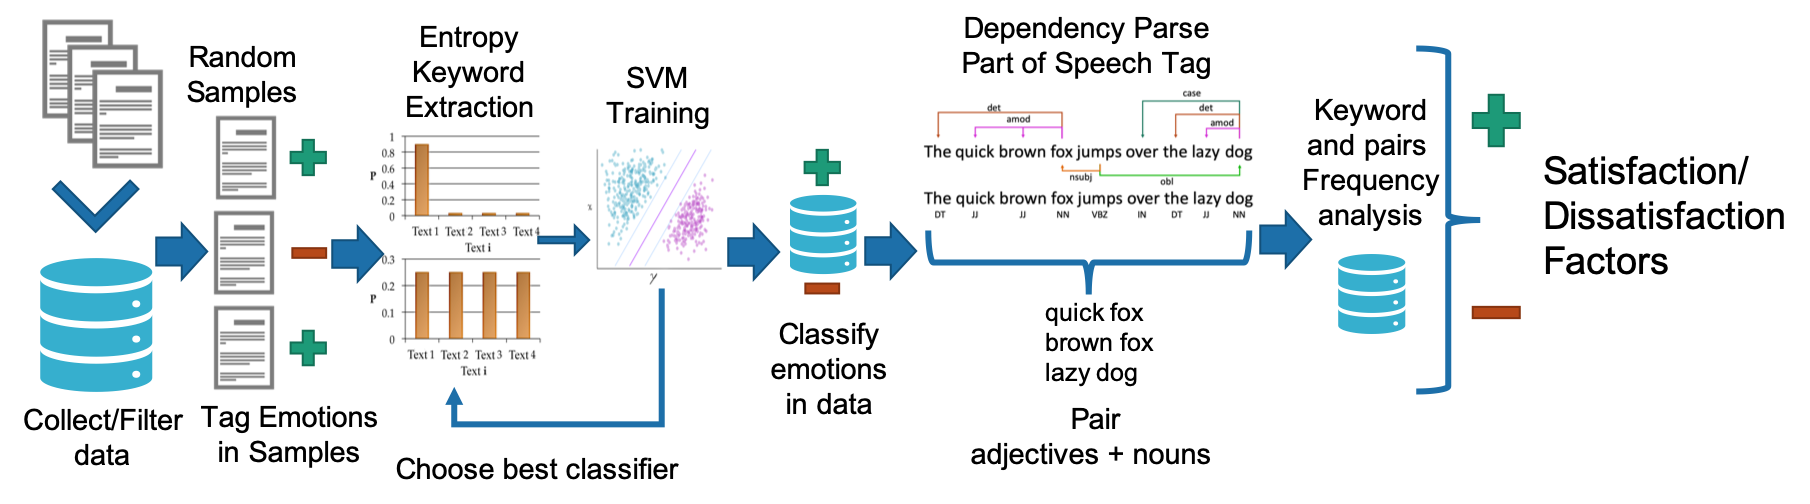
\includegraphics[width=\textwidth]{emotion-method-overview_V3.png}
  \caption{Overview of the methodology to quantitatively rank satisfaction factors.}
  \label{fig:method-overview}
  \end{figure}

  \subsection{Data collection}\label{datacollection}

    In the \DIFdelbegin \DIFdel{data collection stage for Chinese reviews in }\textit{\DIFdel{Ctrip}}%DIFAUXCMD
\DIFdel{, }\DIFdelend \DIFaddbegin \textit{\DIFadd{Ctrip}} \DIFadd{data collection, reviews from }\DIFaddend a total of \num[group-separator={,}]{5774} \DIFdelbegin \DIFdel{review pages of }\DIFdelend hotels in Japan were collected. From these pages, we extracted a total of \num[group-separator={,}]{245919} reviews, from which \num[group-separator={,}]{211932} were detected to be standard Mandarin Chinese\DIFdelbegin \DIFdel{from mainland China}\DIFdelend . Since a single review can have sentences with different sentiments, we separated sentences using punctuation marks. The Chinese reviews were comprised of \num[group-separator={,}]{187348} separate sentences. 

    In the \textit{TripAdvisor} data collection, we collected data from \num[group-separator={,}]{21380} different hotels. In total, we collected \num[group-separator={,}]{295931} reviews, from which \num[group-separator={,}]{295503} were detected to be in English. Similarly to the Chinese data, we then separated these English reviews into \num[group-separator={,}]{2694261} sentences using the \textit{gensim} python library. For the language detection in both cases we used the \textit{langdetect} python library.

    However, \DIFdelbegin \DIFdel{we needed }\DIFdelend to make the data \DIFdelbegin \DIFdel{and comparisons we draw from each of these datasets fair. For that purpose}\DIFdelend \DIFaddbegin \DIFadd{comparisons fair}\DIFaddend , we filtered both databases only to contain reviews from hotels in both datasets, using their English names to do a search match. We also filtered them to be in the same date range\DIFdelbegin \DIFdel{and cut off reviews outside of each other's date ranges}\DIFdelend . In addition, we selected only the hotels that had pricing information available. We extracted the lowest \DIFdelbegin \DIFdel{price possible for a room or bed for one night, and the }\DIFdelend \DIFaddbegin \DIFadd{and }\DIFaddend highest price possible for one night as well. The difference in pricing can be from better room settings, such as double or twin rooms or suites\DIFdelbegin \DIFdel{of several classes}\DIFdelend , depending on the hotel. Regardless of the reason, \DIFaddbegin \DIFadd{we chose }\DIFaddend the highest-priced room \DIFaddbegin \DIFadd{since it }\DIFaddend can be an \DIFaddbegin \DIFadd{indirect }\DIFaddend indicator of the hotel's class\DIFdelbegin \DIFdel{indirectly, giving us insight into the kind of service offered}\DIFdelend . After filtering, \DIFdelbegin \DIFdel{we found that the number of }\DIFdelend \DIFaddbegin \DIFadd{the datasets contained \num[group-separator={,}]{557} }\DIFaddend hotels in common\DIFdelbegin \DIFdel{in the data collected was \num[group-separator={,}]{557}}\DIFdelend . The overlapping date range for reviews was from July 2014 to July 2017. Within these hotels, from \textit{Ctrip} there was \num[group-separator={,}]{48070} reviews comprised of \num[group-separator={,}]{101963} sentences, and from \textit{TripAdvisor} there was \num[group-separator={,}]{41137} reviews comprised of \num[group-separator={,}]{348039} sentences. 
\DIFdelbegin \DIFdel{After filtering the data, we found that the number of reviews was similar for both English and Chinese reviews, but that English reviews tend to be longer in general.
}\DIFdelend 

    The price for a night in these hotels ranges from \DIFdelbegin \DIFdel{low priced }\DIFdelend \DIFaddbegin \DIFadd{cheap }\DIFaddend capsule hotels at 2000 yen per night to high-end hotels \DIFdelbegin \DIFdel{\num[group-separator={,}]{188000} }\DIFdelend \DIFaddbegin \DIFadd{188,000 }\DIFaddend yen a night \DIFdelbegin \DIFdel{as }\DIFdelend \DIFaddbegin \DIFadd{at }\DIFaddend the far ends of the bell curve. Customers' expectations can vary greatly depending on the pricing of the hotel room they stay at. Therefore, we made observations on the distribution of pricing in our database's hotels and binned the data by price ranges, decided by consideration of the objective of stay. We show these distributions in Figure \ref{fig:price_dist}. The structure of the data after division by price is shown in Table \ref{tab:exp_notes}. This table also includes the results of emotional classification after applying our SVC, as explained in \ref{sentimentanalysis}. The first three price ranges (0 to 2500 yen, 2500 to 5000 yen, 5000 to 10,000 yen) would correspond to low-class hotels or even hostels on the lower end and cheap business hotels on the higher end. Further on, there are business hotels in the next range (10,000 to 15,000 yen). After that, the stays could be at Japanese style \textit{ryokan} when traveling in groups, high-class business hotels, luxury love hotels, or higher class hotels (15,000 to 20,000 yen, 20,000 to 30,000 yen). Further than that is more likely to be \textit{ryokan} or high class resorts or five-star hotels (30,000 to 50,000 yen, 50,000 to 100,000 yen, 100,000 to 200,000 yen). Note that because of choosing the highest price per one night in each hotel, the cheapest two price ranges (0 to 2500 yen, 2500 to 5000 yen) are empty, despite some rooms being priced at 2000 yen per night. Because of this, other tables will omit these two price ranges.

    \begin{figure}[ht]
        \centering
        \begin{subfigure}[b]{0.45\textwidth}
            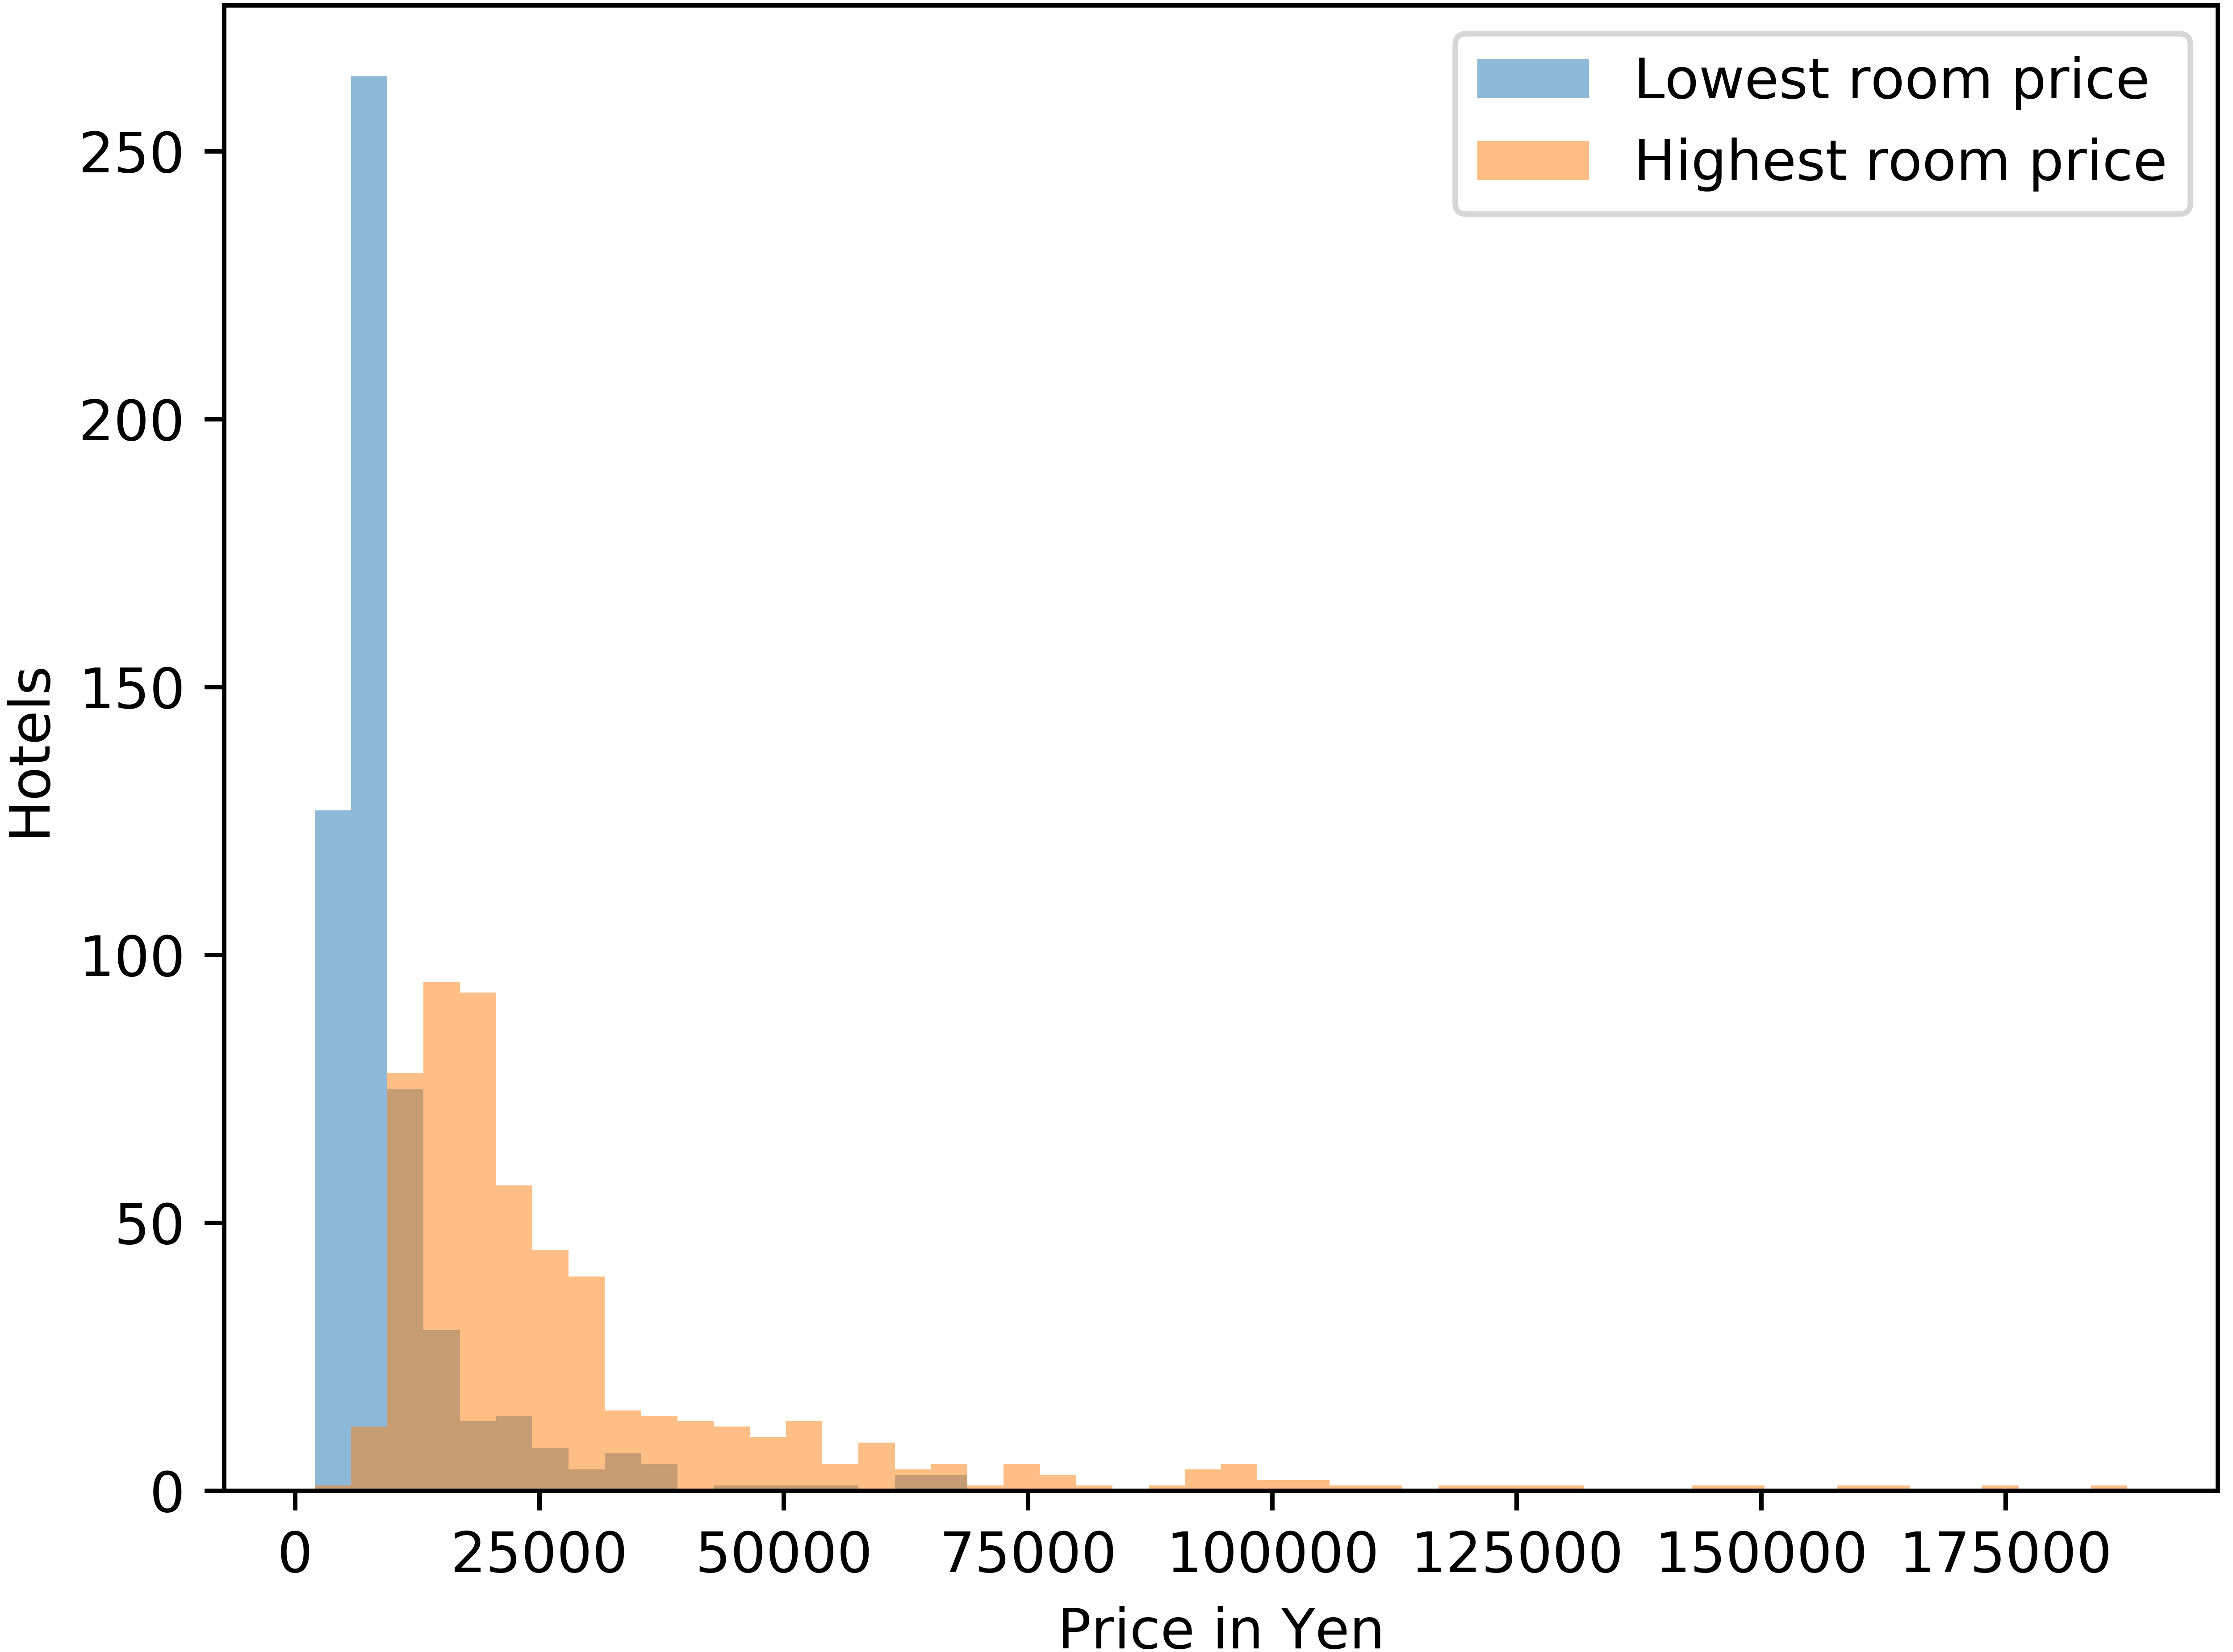
\includegraphics[width=\textwidth]{price_range_distribution_50_even_bins.png}
            \caption{50 equal lenght bins}
        \end{subfigure}
        \begin{subfigure}[b]{0.45\textwidth}
            \includegraphics[width=\textwidth]{price_range_distribution_bins_ver_2.png}
            \caption{manually set 9 price ranges}
        \end{subfigure}
    \caption{Price for one night distribution, blue: lowest price, orange: highest price.}
    \label{fig:price_dist}
    \end{figure}

    % Please add the following required packages to your document preamble:
    % \usepackage{multirow}
    % \usepackage{graphicx}
    \begin{table}[ht]
      \centering
      \caption{Collected data and structure after price range categorizing.}
      \label{tab:exp_notes}
      \resizebox{\textwidth}{!}{%
      \begin{tabular}{|l|l|r|r|}
        \hline
        \multicolumn{1}{|c|}{\textbf{Price range}} & \multicolumn{1}{c|}{\textbf{Data collected}} & \textbf{Ctrip database} & \textbf{Tripadvisor database} \\ \hline
        \multirow{5}{*}{0: All Prices}               & Hotels             & 557     & 557     \\
                                                   & Reviews            & 48,070  & 41,137  \\
                                                   & Sentences          & 101,963 & 348,039 \\
                                                   & Positive sentences & 88,543  & 165,308 \\
                                                   & Negative sentences & 13,420  & 182,731 \\ \hline
        \multirow{2}{*}{1: 0 to 2500 yen}            & Hotels             & 0       & 0       \\
                                                   & Reviews            & 0       & 0       \\ \hline
        \multirow{2}{*}{2: 2500 to 5000 yen}         & Hotels             & 0       & 0       \\
                                                   & Reviews            & 0       & 0       \\ \hline
        \multirow{5}{*}{3: 5000 to 10,000 yen}       & Hotels             & 22      & 22      \\
                                                   & Reviews            & 452     & 459     \\
                                                   & Sentences          & 1,108   & 3,988   \\
                                                   & Positive sentences & 924     & 1,875   \\
                                                   & Negative sentences & 184     & 2,113   \\ \hline
        \multirow{5}{*}{4: 10,000 to 15,000 yen}     & Hotels             & 112     & 112     \\
                                                   & Reviews            & 2,176   & 2,865   \\
                                                   & Sentences          & 4,240   & 24,107  \\
                                                   & Positive sentences & 3,566   & 11,619  \\
                                                   & Negative sentences & 674     & 12,488  \\ \hline
        \multirow{5}{*}{5: 15,000 to 20,000 yen}     & Hotels             & 138     & 138     \\
                                                   & Reviews            & 7,043   & 4,384   \\
                                                   & Sentences          & 14,726  & 37,342  \\
                                                   & Positive sentences & 12,775  & 17,449  \\
                                                   & Negative sentences & 1,951   & 19,893  \\ \hline
        \multirow{5}{*}{6: 20,000 to 30,000 yen}     & Hotels             & 129     & 129     \\
                                                   & Reviews            & 11,845  & 13,772  \\
                                                   & Sentences          & 24,413  & 115,830 \\
                                                   & Positive sentences & 21,068  & 55,381  \\
                                                   & Negative sentences & 3,345   & 60,449  \\ \hline
        \multirow{5}{*}{7: 30,000 to 50,000 yen}     & Hotels             & 83      & 83      \\
                                                   & Reviews            & 8,283   & 7,001   \\
                                                   & Sentences          & 17,939  & 58,409  \\
                                                   & Positive sentences & 15,642  & 28,493  \\
                                                   & Negative sentences & 2,297   & 29,916  \\ \hline
        \multirow{5}{*}{8: 50,000 to 100,000 yen}    & Hotels             & 59      & 59      \\
                                                   & Reviews            & 16,670  & 9,646   \\
                                                   & Sentences          & 36,255  & 81,940  \\
                                                   & Positive sentences & 31,638  & 38,217  \\
                                                   & Negative sentences & 4,617   & 43,723  \\ \hline
        \multirow{5}{*}{9: 100,000 to 200,000 yen}   & Hotels             & 14      & 14      \\
                                                   & Reviews            & 1,601   & 3,010   \\
                                                   & Sentences          & 3,282   & 26,423  \\
                                                   & Positive sentences & 2,930   & 12,274  \\
                                                   & Negative sentences & 352     & 14,149  \\ \hline
        \end{tabular}%
      }
    \end{table}
  \subsection{Text processing}\label{textprocessing}

    \DIFdelbegin \DIFdel{Chinese text, unlike English, does not have spaces between each word to separate them. Besides, we also }\DIFdelend \DIFaddbegin \DIFadd{We }\DIFaddend needed to analyze the grammatical relationship between words, be it English or Chinese, to understand \DIFaddbegin \DIFadd{the }\DIFaddend connections between adjectives and nouns. For all these processes, we used the Stanford CoreNLP pipeline developed by the Natural Language Processing Group at Stanford University \cite[][]{manning-EtAl:2014:P14-5}. In order to separate Chinese words for analysis, we used the Stanford Word Segmenter \cite[][]{chang2008}. In \DIFdelbegin \DIFdel{the case of texts in English }\DIFdelend \DIFaddbegin \DIFadd{English texts}\DIFaddend , however, only using spaces is not enough to correctly collect concepts. The English language is full of variations and conjugations of words depending on the context and tense. Thus, a better segmentation is achieved by using lemmatization, which returns each word's dictionary form. For this purpose, we used the \textit{gensim} library \DIFdelbegin \DIFdel{with }\DIFdelend \DIFaddbegin \DIFadd{for }\DIFaddend the English texts.

    A dependency parser analyzes the grammatical structure, detecting connections between words, and describing the action and direction of those connections. We show an example of these dependencies in Figure \ref{fig:depparse}. This study uses the Stanford NLP Dependency Parser, as described by \cite{chen-EMNLP:2014}. A list of dependencies used by this parser is detailed by \cite{marneffe_manning_2016_depparse_manual}. In more recent versions, they use an updated dependency tag list from Universal Dependencies \cite[][]{zeman2018conll}. In our study, this step was necessary to extract adjective modifiers and their subject. We did that by parsing the \DIFdelbegin \DIFdel{entire }\DIFdelend database and extracting instances of a few determined dependency codes. One of these dependency codes is ``amod'', which stands for ``adjectival modifier''. This is used when an adjective modifies a noun directly (e.g., A big apple). The other dependency code we used was ``nsubj'', or nominal subject, the class's syntactic subject. We used this one for cases where the adjective is modifying the noun indirectly through other words (e.g., The apple is big). This dependency does not necessarily only include a combination of adjectives and nouns. However, it can also be connected with copular verbs, nouns, or other adjectives. We saw it necessary also to perform a Part of Speech (POS) tagging of these clauses.

    \begin{figure}[ht]
    \centering
    \includegraphics[width=0.6\textwidth]{depparse.png}
    \caption{Example of dependency parsing.}
    \label{fig:depparse}
    \end{figure}

    A Part of Speech (POS) tagger is a program that assigns word tokens with tags identifying the part of speech. An example is shown in Figure \ref{fig:postag}. A Part of Speech is a category of lexical items that serve similar grammatical purposes, for example, nouns, adjectives, verbs, or conjunctions. In our study, we used the Stanford NLP POS tagger software, described by \cite{toutanova2000enriching} and \cite{toutanova2003feature}, which uses the Penn Chinese Treebank tags \cite[][]{xia_penntreebank}.

    \begin{figure}[ht]
    \centering
    
\includegraphics[width=0.6\textwidth]{postag.png}
    \caption{Example of POS tagging with the Penn Treebank tags.}
    \label{fig:postag}
    \end{figure}

    In this study, we were interested in identifying combinations of adjectives, some verbs, and nouns. We also needed to filter away bad combinations that were brought by the versatility of nominal subject dependencies. For this purpose, we identified the tags for nouns, verbs, and adjectives in Chinese and English, with the English tags being a bit more varied. What would be called adjectives in English corresponds more to stative verbs in Chinese, so we needed to extract those as well. We show a detailed description of the chosen tags in Table \ref{tab:target_postag}. We also show a detailed description of the tags we needed to filter. We selected these tags heuristically by observing commonly found undesired pairs in Table \ref{tab:filter_postag}.

    % Please add the following required packages to your document preamble:
    % \usepackage{multirow}
    \begin{table}[ht]
      \centering
      \caption{Target Parts of Speech for extraction and pairing.}
      \label{tab:target_postag}
      \resizebox{\textwidth}{!}{%
      \begin{tabular}{|c|c|l|l|}
        \hline
        \textbf{Language}                    & \textbf{POS Tag} & \multicolumn{1}{c|}{\textbf{Part of Speech}} & \multicolumn{1}{c|}{\textbf{Examples}}     \\ \hline
        \multirow{4}{*}{Chinese target tags} & NN               & Noun (general)                               & \begin{CJK}{UTF8}{gbsn}酒店\end{CJK} (hotel) \\ \cline{2-4} 
                                             & VA  & Predicative Adjective (verb)       & \begin{CJK}{UTF8}{gbsn}干净 的\end{CJK} (clean)   \\ \cline{2-4} 
                                             & JJ  & Noun modifier (adjectives)         & \begin{CJK}{UTF8}{gbsn}干净\end{CJK} (clean)     \\ \cline{2-4} 
                                             & VV  & Verb (general)                     & \begin{CJK}{UTF8}{gbsn}推荐\end{CJK} (recommend) \\ \hline
        \multirow{9}{*}{English target tags} & NN  & Noun (general)                     & room                                           \\ \cline{2-4} 
                                             & NNS & Noun (plural)                      & beds                                           \\ \cline{2-4} 
                                             & JJ  & Adjective                          & big                                            \\ \cline{2-4} 
                                             & JJS & Adjective (superlative)            & best                                           \\ \cline{2-4} 
                                             & JJR & Adjective (comparative)            & larger                                         \\ \cline{2-4} 
                                             & VB  & Verb (base form)                   & take                                           \\ \cline{2-4} 
                                             & VBP & Verb (single present)              & take                                           \\ \cline{2-4} 
                                             & VBN & Verb (past participle)             & taken                                          \\ \cline{2-4} 
                                             & VBG & Verb (gerund / present participle) & taking                                         \\ \hline
        \end{tabular}%
        }
    \end{table}

    % Please add the following required packages to your document preamble:
    % \usepackage{multirow}
    \begin{table}[ht]
      \centering
      \caption{Filtered out Parts of Speech to aid pairing.}
      \label{tab:filter_postag}
      \resizebox{\textwidth}{!}{%
      \begin{tabular}{|c|l|l|l|}
        \hline
        \textbf{Language} &
          \multicolumn{1}{c|}{\textbf{POS Tag}} &
          \multicolumn{1}{c|}{\textbf{Part of Speech}} &
          \multicolumn{1}{c|}{\textbf{Examples}} \\ \hline
        \multirow{4}{*}{Commonly filtered tags} & DT    & Determiner         & a, an                                      \\ \cline{2-4} 
                                                & PN    & Pronoun            & I, you, they                               \\ \cline{2-4} 
                                                & CD    & Cardinal Number    & 1, 2, 3, 4, 5                              \\ \cline{2-4} 
                                                & PU    & Punctuation        & .!?                                        \\ \hline
        \multirow{5}{*}{Chinese filtered tags} &
          DEV &
          Particle &
          \begin{CJK}{UTF8}{gbsn}地\end{CJK} (Japan) (adverbial particle) \\ \cline{2-4} 
                                                & NR    & Noun (proper noun) & \begin{CJK}{UTF8}{gbsn}日本\end{CJK} (Japan) \\ \cline{2-4} 
         &
          M &
          Measure word &
          \begin{CJK}{UTF8}{gbsn}个\end{CJK} (general classifier), \begin{CJK}{UTF8}{gbsn}公里\end{CJK} (kilometer) \\ \cline{2-4} 
         &
          SP &
          Sentence-final particle &
          \begin{CJK}{UTF8}{gbsn}他\end{CJK} (he), \begin{CJK}{UTF8}{gbsn}好\end{CJK} (good) \\ \cline{2-4} 
                                                & IJ    & Interjection       & \begin{CJK}{UTF8}{gbsn}啊\end{CJK} (ah)     \\ \hline
        \multirow{3}{*}{English target tags}    & NNP   & Noun (proper noun) & Japan                                      \\ \cline{2-4} 
                                                & PRP\$ & Possessive Pronoun & My, your, her, his                         \\ \cline{2-4} 
                                                & WP    & Wh-pronoun         & What, who                                  \\ \hline
        \end{tabular}%
        }
    \end{table}

    Once we had these adjective + noun or verb + noun pairs, we could determine what the customers referred to in their reviews. With what frequency they use those pairings positively or negatively.

  \subsection{Sentiment analysis using a Support Vector Classifier}\label{sentimentanalysis}

    The sentiment analysis was performed using the methodology described by \cite{Aleman2018ICAROB}. Keywords are determined by a comparison of Shannon's entropy \cite[][]{shannon1948} between two classes by a factor of \(\alpha\) for one class and \(\alpha'\) for the other, and then they are used in an \DIFdelbegin \DIFdel{SVM }\DIFdelend \DIFaddbegin \DIFadd{SVC }\DIFaddend \cite[][]{cortes1995}, optimizing keywords to select the best performing classifier using the \(F_1\)-measure \cite[][]{powers2011}. The selected \DIFdelbegin \DIFdel{SVM }\DIFdelend \DIFaddbegin \DIFadd{SVC }\DIFaddend keywords would then clearly represent the user driving factors leading to positive and negative emotions. We also performed experiments to choose the best value of the parameter C used in the \DIFdelbegin \DIFdel{SVM}\DIFdelend \DIFaddbegin \DIFadd{SVC}\DIFaddend . C is a constant that affects the optimization process when minimizing the error of the separating hyperplane. Low values of C give some freedom of error, which minimizes false positives \DIFdelbegin \DIFdel{. However, depending on the data, it can }\DIFdelend \DIFaddbegin \DIFadd{but can also }\DIFaddend increase false negatives. Inversely, high C values will likely result in minimal false negatives but a possibility of false positives. \DIFdelbegin \DIFdel{SVM }\DIFdelend \DIFaddbegin \DIFadd{SVC }\DIFaddend performance results are displayed in  Tables \ref{tab:svm_f1_zh} and \ref{tab:svm_f1_en}. Examples of tagged sentences are shown in Table \ref{tab:training_examples}. 

    % Please add the following required packages to your document preamble:
    % \usepackage{graphicx}
    \DIFdelbegin %DIFDELCMD < \begin{table}[ht]
%DIFDELCMD <       \centering
%DIFDELCMD <       \caption{Best performing SVC 5-fold cross-validation Chinese text classifiers.}
%DIFDELCMD <       \label{tab:svm_f1_zh}
%DIFDELCMD <       % \resizebox{\textwidth}{!}{%
%DIFDELCMD <       \begin{tabular}{|l|l|l|l|l|}
%DIFDELCMD <         \hline
%DIFDELCMD <         \textbf{Keyword List} &
%DIFDELCMD <           \textbf{\begin{tabular}[c]{@{}l@{}}Classifier\\ emotion\end{tabular}} &
%DIFDELCMD <           \textbf{C} &
%DIFDELCMD <           \begin{tabular}[c]{@{}l@{}}\(F_1\)\\ \(\mu\)\end{tabular} &
%DIFDELCMD <           \begin{tabular}[c]{@{}l@{}}\(F_1\)\\ \(\sigma\)\end{tabular} \\ \hline
%DIFDELCMD <         \begin{tabular}[c]{@{}l@{}}Satisfaction keywords\\ (\(\alpha = 2.75\))\end{tabular} 
%DIFDELCMD <                 & Satisfaction              & 2.5             & 0.91              & 0.01          \\ \hline
%DIFDELCMD <         \begin{tabular}[c]{@{}l@{}}Negative keywords\\ (\(\alpha' = 3.75\))\end{tabular}    
%DIFDELCMD <                 & Dissatisfaction           & 0.5             & 0.67              & 0.11          \\ \hline
%DIFDELCMD <         \begin{tabular}[c]{@{}l@{}}\textbf{Combined}\\ (\(\alpha=2.75\), \(\alpha'=3.75\))\end{tabular} 
%DIFDELCMD <                 & \textbf{Satisfaction}     & \textbf{0.5}    & \textbf{0.95}     & \textbf{0.01} \\ \hline
%DIFDELCMD <         \end{tabular}
%DIFDELCMD <         %
%DIFDELCMD <         % }
%DIFDELCMD <     \end{table}
%DIFDELCMD < %%%
\DIFdelend \DIFaddbegin \begin{table}[ht]
      \centering
      \caption{Best performing SVC 5-fold cross-validation Chinese text classifiers.}
      \label{tab:svm_f1_zh}
      \resizebox{0.65\textwidth}{!}{%
      \begin{tabular}{|l|l|l|l|l|}
        \hline
        \textbf{Keyword List} &
          \textbf{\begin{tabular}[c]{@{}l@{}}Classifier\\ emotion\end{tabular}} &
          \textbf{C} &
          \begin{tabular}[c]{@{}l@{}}\(F_1\)\\ \(\mu\)\end{tabular} &
          \begin{tabular}[c]{@{}l@{}}\(F_1\)\\ \(\sigma\)\end{tabular} \\ \hline
        \begin{tabular}[c]{@{}l@{}}Satisfaction keywords\\ (\(\alpha = 2.75\))\end{tabular} 
                & Satisfaction              & 2.5             & 0.91              & 0.01          \\ \hline
        \begin{tabular}[c]{@{}l@{}}Negative keywords\\ (\(\alpha' = 3.75\))\end{tabular}    
                & Dissatisfaction           & 0.5             & 0.67              & 0.11          \\ \hline
        \begin{tabular}[c]{@{}l@{}}\textbf{Combined}\\ (\(\alpha=2.75\), \(\alpha'=3.75\))\end{tabular} 
                & \textbf{Satisfaction}     & \textbf{0.5}    & \textbf{0.95}     & \textbf{0.01} \\ \hline
        \end{tabular}
        %
        }
    \end{table}
\DIFaddend 

    % Please add the following required packages to your document preamble:
    % \usepackage{graphicx}
    \DIFdelbegin %DIFDELCMD < \begin{table}[ht]
%DIFDELCMD <       \centering
%DIFDELCMD <       \caption{Best performing SVC 10-fold cross-validation English text classifiers.}
%DIFDELCMD <       \label{tab:svm_f1_en}
%DIFDELCMD <       % \resizebox{\textwidth}{!}{%
%DIFDELCMD <       \begin{tabular}{|l|l|l|l|l|}
%DIFDELCMD <         \hline
%DIFDELCMD <         \textbf{Keyword List} &
%DIFDELCMD <           \textbf{\begin{tabular}[c]{@{}l@{}}Classifier\\ emotion\end{tabular}} &
%DIFDELCMD <           \textbf{C} &
%DIFDELCMD <           \begin{tabular}[c]{@{}l@{}}\(F_1\)\\ \(\mu\)\end{tabular} &
%DIFDELCMD <           \begin{tabular}[c]{@{}l@{}}\(F_1\)\\ \(\sigma\)\end{tabular} \\ \hline
%DIFDELCMD <         \begin{tabular}[c]{@{}l@{}}Satisfaction keywords \\ (\(\alpha=1.5\))\end{tabular}       
%DIFDELCMD <                 & Satisfaction              & 1.75            & 0.82              & 0.02          \\ \hline
%DIFDELCMD <         \begin{tabular}[c]{@{}l@{}}Dissatisfaction keywords \\ (\(\alpha'=4.25\))\end{tabular}  
%DIFDELCMD <                 & Dissatisfaction           & 3               & 0.80              & 0.03          \\ \hline
%DIFDELCMD <         \begin{tabular}[c]{@{}l@{}}\textbf{Combined} \\ (\(\alpha=1.5\), \(\alpha'=4.25\))\end{tabular} 
%DIFDELCMD <                 & \textbf{Satisfaction}     & \textbf{2}      & \textbf{0.83}     & \textbf{0.02} \\ \hline
%DIFDELCMD <         \end{tabular}
%DIFDELCMD <         %
%DIFDELCMD <         % }
%DIFDELCMD <     \end{table}
%DIFDELCMD < %%%
\DIFdelend \DIFaddbegin \begin{table}[ht]
      \centering
      \caption{Best performing SVC 10-fold cross-validation English text classifiers.}
      \label{tab:svm_f1_en}
      \resizebox{0.65\textwidth}{!}{%
      \begin{tabular}{|l|l|l|l|l|}
        \hline
        \textbf{Keyword List} &
          \textbf{\begin{tabular}[c]{@{}l@{}}Classifier\\ emotion\end{tabular}} &
          \textbf{C} &
          \begin{tabular}[c]{@{}l@{}}\(F_1\)\\ \(\mu\)\end{tabular} &
          \begin{tabular}[c]{@{}l@{}}\(F_1\)\\ \(\sigma\)\end{tabular} \\ \hline
        \begin{tabular}[c]{@{}l@{}}Satisfaction keywords \\ (\(\alpha=1.5\))\end{tabular}       
                & Satisfaction              & 1.75            & 0.82              & 0.02          \\ \hline
        \begin{tabular}[c]{@{}l@{}}Dissatisfaction keywords \\ (\(\alpha'=4.25\))\end{tabular}  
                & Dissatisfaction           & 3               & 0.80              & 0.03          \\ \hline
        \begin{tabular}[c]{@{}l@{}}\textbf{Combined} \\ (\(\alpha=1.5\), \(\alpha'=4.25\))\end{tabular} 
                & \textbf{Satisfaction}     & \textbf{2}      & \textbf{0.83}     & \textbf{0.02} \\ \hline
        \end{tabular}
        %
        }
    \end{table}
\DIFaddend 

    % Please add the following required packages to your document preamble:
    % \usepackage{multirow}
    % \usepackage{graphicx}
    % \usepackage[normalem]{ulem}
    % \useunder{\uline}{\ul}{}
    \begin{table}[ht]
      \centering
      \caption{Examples of positive and negative sentences used for training SVM.}
      \label{tab:training_examples}
      \resizebox{\textwidth}{!}{%
      \begin{tabular}{|c|c|l|}
        \hline
        \multicolumn{1}{|l|}{\textbf{Language}} &
          \multicolumn{1}{l|}{\textbf{Emotion}} &
          \textbf{Sentences} \\ \hline
        \multirow{4}{*}{Chinese} &
          \multirow{2}{*}{Positive} &
          \begin{tabular}[c]{@{}l@{}}\begin{CJK}{UTF8}{gbsn}酒店 的 服务 很 好 和 我 住 过 的 所有 日本 酒店 一样 各 种 隐形 服务 非常 厉害\end{CJK}\\ (translated as: "The service of the hotel is very good.\\ All the services of the Japanese hotels I have stayed in are extremely good.")\end{tabular} \\ \cline{3-3} 
         &
           &
          \begin{tabular}[c]{@{}l@{}}\begin{CJK}{UTF8}{gbsn}有 一 个 后门 到 地铁站 非常 近 周边 也 算 方便 酒店 服务 和 卫生 都 很 好\end{CJK}\\ (translated as: "There is a back door to the subway station very close to it. \\ The surrounding area is also convenient hotel service and health are very good")\end{tabular} \\ \cline{2-3} 
         &
          \multirow{2}{*}{Negative} &
          \begin{tabular}[c]{@{}l@{}}\begin{CJK}{UTF8}{gbsn}酒店 旁边 很 荒凉 连个 便利 店 都 要 走 很远\end{CJK}\\ (translated as: "The hotel is very bleak, \\ and you have to go very far to go to the nearest convenience store.")\end{tabular} \\ \cline{3-3} 
         &
           &
          \begin{tabular}[c]{@{}l@{}}\begin{CJK}{UTF8}{gbsn}唯一 不 足 是 价格 太高\end{CJK}\\ (translated as: "The only negative is that the price is too high.")\end{tabular} \\ \hline
        \multirow{4}{*}{English} &
          \multirow{2}{*}{Positive} &
          It was extremely clean, peaceful and the hotel Hosts made us feel super welcome \\ \cline{3-3} 
         &
           &
          \begin{tabular}[c]{@{}l@{}}Location is very good, close to a main road with a subway station, a bakery,\\  a 7 eleven and a nice restaurant that is not too expensive but serves good food\end{tabular} \\ \cline{2-3} 
         &
          \multirow{2}{*}{Negative} &
          \begin{tabular}[c]{@{}l@{}}The only downside. Our room was labeled 'non-smoking'\\ but our duvet reeked of smoke.\end{tabular} \\ \cline{3-3} 
         &
           &
          A bit pricey though \\ \hline
        \end{tabular}%
        }
    \end{table}

    Shannon's entropy can be used to observe the probability distribution of each word inside the corpus. A word included in many documents will have a high entropy value for that set of documents. Opposite to this, a word appearing in only one document will have an entropy value of zero. 

    An \DIFdelbegin \DIFdel{SVM }\DIFdelend \DIFaddbegin \DIFadd{SVC }\DIFaddend is trained to classify data based on previously labeled data, generalizing the data's features by defining a separating (p-1)-dimensional hyperplane in p-dimensional space. Each dimension is a feature of the data in this space. The separating hyperplane, along with the support vectors, divides the multi-dimensional space and minimizes classification error. 

    Our study used \DIFdelbegin \DIFdel{the SVM classification process's linear kernel }\DIFdelend \DIFaddbegin \DIFadd{a linear kernel for the SVC}\DIFaddend , defined by the formula (\ref{eq:svm1}) below. Each training sentence is a data point, a row in the vector \(x\). Each column represents a feature; in our case, the quantities of each of the keywords in that particular sentence. The labels of previously known classifications (1 for positive, 0 for negative) for each sentence comprise the \(f(x)\) vector. The Weight Vector \(w\) is comprised of the influences each point has had in the training process to define the hyperplane angle. The bias coefficient \(b\) determines its position.

    During the \DIFdelbegin \DIFdel{SVM }\DIFdelend \DIFaddbegin \DIFadd{SVC }\DIFaddend learning algorithm, each data point classified incorrectly \DIFdelbegin \DIFdel{causes a change in }\DIFdelend \DIFaddbegin \DIFadd{alters }\DIFaddend the weight vector to correctly classify new data. These changes to the weight vector are greater for features close to the separating hyperplane. These features have stronger changes because they needed to be taken into account to classify with a minimal error. Sequentially, the weight vector can be interpreted as a numerical representation of each feature's effect on each class's classification process. Below we show the formula for the weight vector \(w\) (\ref{eq:svm_weight}), where \(x\) is the training data and each vectorized sentence \(x_i\) in the data is labeled \(y_i\). Each cycle of the algorithm alters the value of \(w\) by \(\alpha\) to reduce the number of wrong classifications. This equation shows the last value of \(\alpha\) after the end of the cycle.

    \begin{equation}\label{eq:svm1}
    f(x) = w^\top x + b
    \end{equation}

    \begin{equation}\label{eq:svm_weight}
    w = \sum_{i=1}^N \alpha_i y_i x_i
    \end{equation}

    We tagged 159 Chinese sentences and \num[group-separator={,}]{2357} English sentences as positive or negative for our training data. The entropy comparison factors \(\alpha\) and \(\alpha'\) were tested from 1.25 to 6 in intervals of 0.25. We applied this SVC to classify the rest of our data collection. Subsequently, the positive and negative sentence counts shown in Table \ref{tab:exp_notes} result from applying our SVC for classification.

\section{Data Analysis}\label{dataanalysis}

  \subsection{Frequent keywords in differently priced hotels}\label{svmresults}

    \DIFdelbegin \DIFdel{To understand Chinese tourists and English-speaking tourists' satisfaction and dissatisfaction factors when lodging in Japan, we study both the frequency of the words they use. Following that, to know the relevance of a keyword as a preference for each group, we observed each entropy-based keyword's frequencies in our complete data set and in each price range. The frequency of the keywords in the database shows the level of priority it has for customers.
}%DIFDELCMD < 

%DIFDELCMD <     %%%
\DIFdelend We observed the top 10 \DIFdelbegin \DIFdel{words }\DIFdelend \DIFaddbegin \DIFadd{satisfaction and dissatisfaction keywords }\DIFaddend with the highest frequencies \DIFdelbegin \DIFdel{for keywords linked by entropy to satisfaction and dissatisfaction in }\DIFdelend \DIFaddbegin \DIFadd{of }\DIFaddend emotionally positive and negative statements to study. The keywords are the quantitative rank of the needs of Chinese and \DIFdelbegin \DIFdel{English speaking }\DIFdelend \DIFaddbegin \DIFadd{English-speaking }\DIFaddend customers. We show the top 10 positive keywords for each price range comparing English and Chinese in Table \ref{tab:freq_res_pos}. For the negative keywords, we show the results in Table \ref{tab:freq_res_neg}.

    We can observe that the most used keywords for most price ranges in the same language are similar, with a few changes in priority for the keywords involved. For example, in Chinese, we can see that the customers praise cleanliness first in cheaper hotels, whereas the size of the room or bed is praised more in hotels of higher class. Another example is that in negative English reviews, complaints about price appear only after 10,000 yen hotels. After this, it climbs in importance following the increase in the hotel's price.


    % Please add the following required packages to your document preamble:
    % \usepackage{multirow}
    % \usepackage{graphicx}
    % \usepackage[normalem]{ulem}
    % \useunder{\uline}{\ul}{}
    \begin{table}[ht]
      \centering
      \caption{English and Chinese comparison of the top 10 positive keywords.}
      \label{tab:freq_res_pos}
      \resizebox{\textwidth}{!}{%
      \begin{tabular}{|c|lr|lr|}
        \hline
        \textbf{Price range} &
          \multicolumn{1}{c|}{\textbf{Chinese keyword}} &
          \multicolumn{1}{c|}{\textbf{Counts in Ctrip}} &
          \multicolumn{1}{c|}{\textbf{English keyword}} &
          \multicolumn{1}{c|}{\textbf{Counts in Tripadvisor}} \\ \hline
        \multirow{10}{*}{\textbf{0: All Prices}}             & \begin{CJK}{UTF8}{gbsn}不错\end{CJK} (not bad)         & 12892 & good        & 19148 \\  
                                                             & \begin{CJK}{UTF8}{gbsn}大\end{CJK} (big)              & 9844  & staff       & 16289 \\  
                                                             & \begin{CJK}{UTF8}{gbsn}干净\end{CJK} (clean)           & 6665  & great       & 16127 \\  
                                                             & \begin{CJK}{UTF8}{gbsn}交通\end{CJK} (traffic)         & 6560  & location    & 11838 \\  
                                                             & \begin{CJK}{UTF8}{gbsn}早餐\end{CJK} (breakfast)       & 5605  & nice        & 11615 \\  
                                                             & \begin{CJK}{UTF8}{gbsn}近\end{CJK} (near)             & 5181  & clean       & 9064  \\  
                                                             & \begin{CJK}{UTF8}{gbsn}地铁\end{CJK} (subway)          & 4321  & helpful     & 5846  \\  
                                                             & \begin{CJK}{UTF8}{gbsn}购物\end{CJK} (shopping)        & 4101  & excellent   & 5661  \\  
                                                             & \begin{CJK}{UTF8}{gbsn}推荐\end{CJK} (recommend)       & 3281  & comfortable & 5625  \\  
                                                             & \begin{CJK}{UTF8}{gbsn}环境\end{CJK} (environment)    & 3258  & friendly    & 5606  \\ \hline
        \multirow{10}{*}{\textbf{3: 5000 to 10,000 yen}}     & \begin{CJK}{UTF8}{gbsn}不错\end{CJK} (not bad)         & 139   & good        & 206   \\  
                                                             & \begin{CJK}{UTF8}{gbsn}干净\end{CJK} (clean)           & 114   & staff       & 181   \\  
                                                             & \begin{CJK}{UTF8}{gbsn}早餐\end{CJK} (breakfast)       & 112   & clean       & 174   \\  
                                                             & \begin{CJK}{UTF8}{gbsn}大\end{CJK} (big)              & 76    & nice        & 166   \\  
                                                             & \begin{CJK}{UTF8}{gbsn}交通\end{CJK} (traffic)         & 72    & great       & 143   \\  
                                                             & \begin{CJK}{UTF8}{gbsn}地铁\end{CJK} (subway)          & 66    & location    & 91    \\  
                                                             & \begin{CJK}{UTF8}{gbsn}近\end{CJK} (near)             & 55    & comfortable & 79    \\  
                                                             & \begin{CJK}{UTF8}{gbsn}地铁站\end{CJK} (subway station) & 51    & helpful     & 70    \\  
                                                             & \begin{CJK}{UTF8}{gbsn}远\end{CJK} (far)              & 41    & friendly    & 64    \\  
                                                             & \begin{CJK}{UTF8}{gbsn}附近\end{CJK} (nearby)          & 34    & recommend   & 59    \\ \hline
        \multirow{10}{*}{\textbf{4: 10,000 to 15,000 yen}}   & \begin{CJK}{UTF8}{gbsn}不错\end{CJK} (not bad)         & 601   & good        & 1399  \\  
                                                             & \begin{CJK}{UTF8}{gbsn}干净\end{CJK} (clean)           & 455   & staff       & 1165  \\  
                                                             & \begin{CJK}{UTF8}{gbsn}大\end{CJK} (big)              & 348   & great       & 961   \\  
                                                             & \begin{CJK}{UTF8}{gbsn}近\end{CJK} (near)             & 323   & nice        & 808   \\  
                                                             & \begin{CJK}{UTF8}{gbsn}早餐\end{CJK} (breakfast)       & 270   & location    & 800   \\  
                                                             & \begin{CJK}{UTF8}{gbsn}卫生\end{CJK} (health)          & 201   & clean       & 656   \\  
                                                             & \begin{CJK}{UTF8}{gbsn}交通\end{CJK} (traffic)         & 196   & excellent   & 412   \\  
                                                             & \begin{CJK}{UTF8}{gbsn}地铁\end{CJK} (subway)          & 164   & friendly    & 400   \\  
                                                             & \begin{CJK}{UTF8}{gbsn}远\end{CJK} (far)              & 158   & helpful     & 393   \\  
                                                             & \begin{CJK}{UTF8}{gbsn}附近\end{CJK} (nearby)          & 150   & comfortable & 391   \\ \hline
        \multirow{10}{*}{\textbf{5: 15,000 to 20,000 yen}}   & \begin{CJK}{UTF8}{gbsn}不错\end{CJK} (not bad)         & 1925  & good        & 2242  \\  
                                                             & \begin{CJK}{UTF8}{gbsn}干净\end{CJK} (clean)           & 1348  & staff       & 1674  \\  
                                                             & \begin{CJK}{UTF8}{gbsn}大\end{CJK} (big)              & 1277  & great       & 1414  \\  
                                                             & \begin{CJK}{UTF8}{gbsn}交通\end{CJK} (traffic)         & 1058  & clean       & 1204  \\  
                                                             & \begin{CJK}{UTF8}{gbsn}近\end{CJK} (near)             & 1016  & nice        & 1175  \\  
                                                             & \begin{CJK}{UTF8}{gbsn}地铁\end{CJK} (subway)          & 801   & location    & 1109  \\  
                                                             & \begin{CJK}{UTF8}{gbsn}早餐\end{CJK} (breakfast)       & 777   & comfortable & 621   \\  
                                                             & \begin{CJK}{UTF8}{gbsn}地铁站\end{CJK} (subway station) & 639   & friendly    & 615   \\  
                                                             & \begin{CJK}{UTF8}{gbsn}附近\end{CJK} (nearby)          & 572   & free        & 581   \\  
                                                             & \begin{CJK}{UTF8}{gbsn}购物\end{CJK} (shopping)        & 516   & helpful     & 552   \\ \hline
        \multirow{10}{*}{\textbf{6: 20,000 to 30,000 yen}}   & \begin{CJK}{UTF8}{gbsn}不错\end{CJK} (not bad)         & 3110  & good        & 6550  \\  
                                                             & \begin{CJK}{UTF8}{gbsn}大\end{CJK} (big)              & 2245  & staff       & 5348  \\  
                                                             & \begin{CJK}{UTF8}{gbsn}交通\end{CJK} (traffic)         & 1990  & great       & 5074  \\  
                                                             & \begin{CJK}{UTF8}{gbsn}干净\end{CJK} (clean)           & 1940  & location    & 4414  \\  
                                                             & \begin{CJK}{UTF8}{gbsn}近\end{CJK} (near)             & 1433  & nice        & 3451  \\  
                                                             & \begin{CJK}{UTF8}{gbsn}地铁\end{CJK} (subway)          & 1073  & clean       & 3364  \\  
                                                             & \begin{CJK}{UTF8}{gbsn}早餐\end{CJK} (breakfast)       & 1007  & shopping    & 1992  \\  
                                                             & \begin{CJK}{UTF8}{gbsn}购物\end{CJK} (shopping)        & 979   & helpful     & 1970  \\  
                                                             & \begin{CJK}{UTF8}{gbsn}周边\end{CJK} (surroundings)    & 837   & comfortable & 1941  \\  
                                                             & \begin{CJK}{UTF8}{gbsn}附近\end{CJK} (nearby)          & 825   & friendly    & 1915  \\ \hline
        \multirow{10}{*}{\textbf{7: 30,000 to 50,000 yen}}   & \begin{CJK}{UTF8}{gbsn}不错\end{CJK} (not bad)         & 2291  & good        & 3407  \\  
                                                             & \begin{CJK}{UTF8}{gbsn}大\end{CJK} (big)              & 1913  & staff       & 2867  \\  
                                                             & \begin{CJK}{UTF8}{gbsn}干净\end{CJK} (clean)           & 1159  & great       & 2620  \\  
                                                             & \begin{CJK}{UTF8}{gbsn}交通\end{CJK} (traffic)         & 1105  & location    & 2186  \\  
                                                             & \begin{CJK}{UTF8}{gbsn}近\end{CJK} (near)             & 935   & nice        & 2160  \\  
                                                             & \begin{CJK}{UTF8}{gbsn}早餐\end{CJK} (breakfast)       & 846   & clean       & 1750  \\  
                                                             & \begin{CJK}{UTF8}{gbsn}推荐\end{CJK} (recommend)       & 638   & helpful     & 1147  \\  
                                                             & \begin{CJK}{UTF8}{gbsn}购物\end{CJK} (shopping)        & 636   & train       & 1040  \\  
                                                             & \begin{CJK}{UTF8}{gbsn}周边\end{CJK} (surroundings)    & 552   & subway      & 1034  \\  
                                                             & \begin{CJK}{UTF8}{gbsn}环境\end{CJK} (environment)    & 541   & friendly    & 1001  \\ \hline
        \multirow{10}{*}{\textbf{8: 50,000 to 100,000 yen}}  & \begin{CJK}{UTF8}{gbsn}不错\end{CJK} (not bad)         & 4451  & great       & 4425  \\  
                                                             & \begin{CJK}{UTF8}{gbsn}大\end{CJK} (big)              & 3670  & good        & 4350  \\  
                                                             & \begin{CJK}{UTF8}{gbsn}早餐\end{CJK} (breakfast)       & 2422  & staff       & 3777  \\  
                                                             & \begin{CJK}{UTF8}{gbsn}交通\end{CJK} (traffic)         & 2012  & nice        & 2991  \\  
                                                             & \begin{CJK}{UTF8}{gbsn}购物\end{CJK} (shopping)        & 1764  & location    & 2439  \\  
                                                             & \begin{CJK}{UTF8}{gbsn}新\end{CJK} (new)              & 1634  & clean       & 1655  \\  
                                                             & \begin{CJK}{UTF8}{gbsn}棒\end{CJK} (great)            & 1626  & excellent   & 1555  \\  
                                                             & \begin{CJK}{UTF8}{gbsn}地铁\end{CJK} (subway)          & 1604  & helpful     & 1313  \\  
                                                             & \begin{CJK}{UTF8}{gbsn}干净\end{CJK} (clean)           & 1577  & comfortable & 1246  \\  
                                                             & \begin{CJK}{UTF8}{gbsn}近\end{CJK} (near)             & 1354  & friendly    & 1238  \\ \hline
        \multirow{10}{*}{\textbf{9: 100,000 to 200,000 yen}} & \begin{CJK}{UTF8}{gbsn}不错\end{CJK} (not bad)         & 375   & great       & 1488  \\  
                                                             & \begin{CJK}{UTF8}{gbsn}大\end{CJK} (big)              & 315   & staff       & 1277  \\  
                                                             & \begin{CJK}{UTF8}{gbsn}棒\end{CJK} (great)            & 189   & good        & 994   \\  
                                                             & \begin{CJK}{UTF8}{gbsn}早餐\end{CJK} (breakfast)       & 171   & nice        & 864   \\  
                                                             & \begin{CJK}{UTF8}{gbsn}环境\end{CJK} (environment)    & 157   & location    & 799   \\  
                                                             & \begin{CJK}{UTF8}{gbsn}交通\end{CJK} (traffic)         & 127   & excellent   & 631   \\  
                                                             & \begin{CJK}{UTF8}{gbsn}选择\end{CJK} (select)          & 112   & beautiful   & 455   \\  
                                                             & \begin{CJK}{UTF8}{gbsn}推荐\end{CJK} (recommend)       & 109   & large       & 404   \\  
                                                             & \begin{CJK}{UTF8}{gbsn}赞\end{CJK} (awesome)          & 101   & helpful     & 401   \\  
                                                             & \begin{CJK}{UTF8}{gbsn}购物\end{CJK} (shopping)        & 98    & wonderful   & 372   \\ \hline
        \end{tabular}%
        }
    \end{table}


    % Please add the following required packages to your document preamble:
    % \usepackage{multirow}
    % \usepackage{graphicx}
    \begin{table}[ht]
      \centering
      \caption{English and Chinese comparison of the top 10 negative keywords.}
      \label{tab:freq_res_neg}
      \resizebox{\textwidth}{!}{%
      \begin{tabular}{|c|lr|lr|}
        \hline
        \textbf{Price range} &
          \multicolumn{1}{c|}{\textbf{Chinese keyword}} &
          \multicolumn{1}{c|}{\textbf{Counts in Ctrip}} &
          \multicolumn{1}{c|}{\textbf{English keyword}} &
          \multicolumn{1}{c|}{\textbf{Counts in Tripadvisor}} \\ \hline
        \multirow{10}{*}{\textbf{0: All Prices}}             & \begin{CJK}{UTF8}{gbsn}价格\end{CJK} (price)     & 1838 & pricey         & 462 \\  
                                                             & \begin{CJK}{UTF8}{gbsn}一般\end{CJK} (general)   & 1713 & poor           & 460 \\  
                                                             & \begin{CJK}{UTF8}{gbsn}中文\end{CJK} (Chinese)   & 733  & dated          & 431 \\  
                                                             & \begin{CJK}{UTF8}{gbsn}地理\end{CJK} (geography) & 691  & disappointing  & 376 \\  
                                                             & \begin{CJK}{UTF8}{gbsn}距离\end{CJK} (distance)  & 434  & worst          & 327 \\  
                                                             & \begin{CJK}{UTF8}{gbsn}陈旧\end{CJK} (obsolete)  & 319  & minor          & 258 \\  
                                                             & \begin{CJK}{UTF8}{gbsn}老\end{CJK} (old)        & 297  & uncomfortable  & 253 \\  
                                                             & \begin{CJK}{UTF8}{gbsn}华人\end{CJK} (Chinese)   & 15   & carpet         & 240 \\  
                                                             &                                                &      & annoying       & 220 \\  
                                                             &                                                &      & sense          & 220 \\ \hline
        \multirow{10}{*}{\textbf{3: 5000 to 10,000 yen}}     & \begin{CJK}{UTF8}{gbsn}价格\end{CJK} (price)     & 31   & worst          & 6   \\  
                                                             & \begin{CJK}{UTF8}{gbsn}一般\end{CJK} (general)   & 28   & walkway        & 5   \\  
                                                             & \begin{CJK}{UTF8}{gbsn}距离\end{CJK} (distance)  & 11   & unable         & 4   \\  
                                                             & \begin{CJK}{UTF8}{gbsn}地理\end{CJK} (geography) & 10   & worse          & 4   \\  
                                                             & \begin{CJK}{UTF8}{gbsn}中文\end{CJK} (Chinese)   & 9    & annoying       & 3   \\  
                                                             & \begin{CJK}{UTF8}{gbsn}老\end{CJK} (old)        & 2    & dirty          & 3   \\  
                                                             &                                                &      & funny smell    & 3   \\  
                                                             &                                                &      & poor           & 3   \\  
                                                             &                                                &      & renovation     & 3   \\  
                                                             &                                                &      & carpet         & 2   \\ \hline
        \multirow{10}{*}{\textbf{4: 10,000 to 15,000 yen}}   & \begin{CJK}{UTF8}{gbsn}价格\end{CJK} (price)     & 98   & dated          & 40  \\  
                                                             & \begin{CJK}{UTF8}{gbsn}一般\end{CJK} (general)   & 91   & poor           & 29  \\  
                                                             & \begin{CJK}{UTF8}{gbsn}距离\end{CJK} (distance)  & 43   & disappointing  & 26  \\  
                                                             & \begin{CJK}{UTF8}{gbsn}陈旧\end{CJK} (obsolete)  & 34   & worst          & 24  \\  
                                                             & \begin{CJK}{UTF8}{gbsn}地理\end{CJK} (geography) & 31   & uncomfortable  & 23  \\  
                                                             & \begin{CJK}{UTF8}{gbsn}老\end{CJK} (old)        & 30   & cigarette      & 22  \\  
                                                             & \begin{CJK}{UTF8}{gbsn}中文\end{CJK} (Chinese)   & 26   & pricey         & 22  \\  
                                                             &                                                &      & minor          & 21  \\  
                                                             &                                                &      & paper          & 19  \\  
                                                             &                                                &      & unable         & 19  \\ \hline
        \multirow{10}{*}{\textbf{5: 15,000 to 20,000 yen}}   & \begin{CJK}{UTF8}{gbsn}价格\end{CJK} (price)     & 296  & poor           & 57  \\  
                                                             & \begin{CJK}{UTF8}{gbsn}一般\end{CJK} (general)   & 218  & dated          & 41  \\  
                                                             & \begin{CJK}{UTF8}{gbsn}地理\end{CJK} (geography) & 125  & disappointing  & 38  \\  
                                                             & \begin{CJK}{UTF8}{gbsn}中文\end{CJK} (Chinese)   & 93   & annoying       & 36  \\  
                                                             & \begin{CJK}{UTF8}{gbsn}距离\end{CJK} (distance)  & 84   & worst          & 36  \\  
                                                             & \begin{CJK}{UTF8}{gbsn}陈旧\end{CJK} (obsolete)  & 43   & cigarette      & 31  \\  
                                                             & \begin{CJK}{UTF8}{gbsn}老\end{CJK} (old)        & 26   & rude           & 28  \\  
                                                             & \begin{CJK}{UTF8}{gbsn}华人\end{CJK} (Chinese)   & 3    & uncomfortable  & 26  \\  
                                                             &                                                &      & paper          & 25  \\  
                                                             &                                                &      & pricey         & 24  \\ \hline
        \multirow{10}{*}{\textbf{6: 20,000 to 30,000 yen}}   & \begin{CJK}{UTF8}{gbsn}一般\end{CJK} (general)   & 504  & poor           & 136 \\  
                                                             & \begin{CJK}{UTF8}{gbsn}价格\end{CJK} (price)     & 472  & dated          & 131 \\  
                                                             & \begin{CJK}{UTF8}{gbsn}地理\end{CJK} (geography) & 164  & pricey         & 120 \\  
                                                             & \begin{CJK}{UTF8}{gbsn}中文\end{CJK} (Chinese)   & 155  & disappointing  & 112 \\  
                                                             & \begin{CJK}{UTF8}{gbsn}距离\end{CJK} (distance)  & 116  & uncomfortable  & 103 \\  
                                                             & \begin{CJK}{UTF8}{gbsn}陈旧\end{CJK} (obsolete)  & 75   & minor          & 93  \\  
                                                             & \begin{CJK}{UTF8}{gbsn}老\end{CJK} (old)        & 55   & smallest       & 88  \\  
                                                             & \begin{CJK}{UTF8}{gbsn}华人\end{CJK} (Chinese)   & 2    & worst          & 86  \\  
                                                             &                                                &      & cigarette      & 79  \\  
                                                             &                                                &      & annoying       & 70  \\ \hline
        \multirow{10}{*}{\textbf{7: 30,000 to 50,000 yen}}   & \begin{CJK}{UTF8}{gbsn}价格\end{CJK} (price)     & 326  & poor           & 92  \\  
                                                             & \begin{CJK}{UTF8}{gbsn}一般\end{CJK} (general)   & 311  & pricey         & 92  \\  
                                                             & \begin{CJK}{UTF8}{gbsn}地理\end{CJK} (geography) & 110  & dated          & 65  \\  
                                                             & \begin{CJK}{UTF8}{gbsn}中文\end{CJK} (Chinese)   & 94   & worst          & 64  \\  
                                                             & \begin{CJK}{UTF8}{gbsn}陈旧\end{CJK} (obsolete)  & 71   & carpet         & 55  \\  
                                                             & \begin{CJK}{UTF8}{gbsn}距离\end{CJK} (distance)  & 68   & uncomfortable  & 55  \\  
                                                             & \begin{CJK}{UTF8}{gbsn}老\end{CJK} (old)        & 45   & dirty          & 51  \\  
                                                             & \begin{CJK}{UTF8}{gbsn}华人\end{CJK} (Chinese)   & 2    & disappointing  & 50  \\  
                                                             &                                                &      & cigarette      & 46  \\  
                                                             &                                                &      & unable         & 43  \\ \hline
        \multirow{10}{*}{\textbf{8: 50,000 to 100,000 yen}} &
                                                               \begin{CJK}{UTF8}{gbsn}价格\end{CJK} (price)     & 561  & pricey         & 163 \\ 
                                                             & \begin{CJK}{UTF8}{gbsn}一般\end{CJK} (general)   & 510  & dated          & 150 \\  
                                                             & \begin{CJK}{UTF8}{gbsn}中文\end{CJK} (Chinese)   & 337  & disappointing  & 129 \\  
                                                             & \begin{CJK}{UTF8}{gbsn}地理\end{CJK} (geography) & 239  & poor           & 124 \\  
                                                             & \begin{CJK}{UTF8}{gbsn}老\end{CJK} (old)        & 134  & worst          & 98  \\  
                                                             & \begin{CJK}{UTF8}{gbsn}距离\end{CJK} (distance)  & 97   & walkway        & 82  \\  
                                                             & \begin{CJK}{UTF8}{gbsn}陈旧\end{CJK} (obsolete)  & 90   & carpet         & 71  \\  
                                                             & \begin{CJK}{UTF8}{gbsn}华人\end{CJK} (Chinese)   & 8    & minor          & 63  \\  
                                                             &                                                &      & sense          & 63  \\  
                                                             &                                                &      & outdated       & 58  \\ \hline
        \multirow{10}{*}{\textbf{9: 100,000 to 200,000 yen}} & \begin{CJK}{UTF8}{gbsn}价格\end{CJK} (price)     & 54   & pricey         & 40  \\  
                                                             & \begin{CJK}{UTF8}{gbsn}一般\end{CJK} (general)   & 51   & sense          & 34  \\  
                                                             & \begin{CJK}{UTF8}{gbsn}中文\end{CJK} (Chinese)   & 19   & minor          & 33  \\  
                                                             & \begin{CJK}{UTF8}{gbsn}距离\end{CJK} (distance)  & 15   & lighting       & 20  \\  
                                                             & \begin{CJK}{UTF8}{gbsn}地理\end{CJK} (geography) & 12   & disappointing  & 19  \\  
                                                             & \begin{CJK}{UTF8}{gbsn}陈旧\end{CJK} (obsolete)  & 6    & poor           & 19  \\  
                                                             & \begin{CJK}{UTF8}{gbsn}老\end{CJK} (old)        & 5    & annoying       & 16  \\  
                                                             &                                                &      & mixed          & 15  \\  
                                                             &                                                &      & disappointment & 14  \\  
                                                             &                                                &      & paper          & 14  \\ \hline
        \end{tabular}%
        }
    \end{table}

  \subsection{Frequently used adjectives and their pairs}\label{adjresults}

    Some keywords in these lists are adjectives, such as the word ``\begin{CJK}{UTF8}{gbsn}大\end{CJK} (big)'' mentioned before. To understand those, we performed the dependency parsing \DIFdelbegin \DIFdel{, }\DIFdelend and part of speech tagging explained in section \ref{textprocessing}. While many of these connections, we only considered the top 4 used keyword connections per adjective per price range. We show the most used Chinese adjectives in positive keywords in Table \ref{tab:adj_zh_pos}, and for negative Chinese adjective keywords in Table \ref{tab:adj_zh_neg}. Similarly, for English adjectives used in positive sentences we show the most common examples in Table \ref{tab:adj_en_pos}, and for adjectives used in negative sentences in Table \ref{tab:adj_en_neg}.

    %%%%%%%%%%%%% POSITIVE CHINESE ADJECTIVE PAIRS
    % Please add the following required packages to your document preamble:
    % \usepackage{multirow}
    % \usepackage{graphicx}
    % \usepackage{lscape}
    \begin{landscape}
    \begin{table}[p]
      \centering
      \caption{Top 4 words related to the mainly used adjectives in positive Chinese texts.}
      \label{tab:adj_zh_pos}
      \resizebox{\linewidth}{!}{%
      \begin{tabular}{|c|l|l|l|l|l|l|}
        \hline
        \textbf{Price range} &
          \multicolumn{1}{c|}{\textbf{\begin{CJK}{UTF8}{gbsn}不错\end{CJK} (not bad)}} &
          \multicolumn{1}{c|}{\textbf{\begin{CJK}{UTF8}{gbsn}大\end{CJK} (big)}} &
          \multicolumn{1}{c|}{\textbf{\begin{CJK}{UTF8}{gbsn}干净\end{CJK} (clean)}} &
          \multicolumn{1}{c|}{\textbf{\begin{CJK}{UTF8}{gbsn}近\end{CJK} (near)}} &
          \multicolumn{1}{c|}{\textbf{\begin{CJK}{UTF8}{gbsn}新\end{CJK} (new)}} &
          \multicolumn{1}{c|}{\textbf{\begin{CJK}{UTF8}{gbsn}棒\end{CJK} (great)}} \\ \hline
        \multirow{5}{*}{\textbf{0: All Prices}} &
          \begin{CJK}{UTF8}{gbsn}不错\end{CJK} (not bad) : 12892 &
          \begin{CJK}{UTF8}{gbsn}大\end{CJK} (big) : 9844 &
          \begin{CJK}{UTF8}{gbsn}干净\end{CJK} (clean) : 6665 &
          \begin{CJK}{UTF8}{gbsn}近\end{CJK} (near) : 5181 &
          \begin{CJK}{UTF8}{gbsn}新\end{CJK} (new) : 2775 &
          \begin{CJK}{UTF8}{gbsn}棒\end{CJK} (great) : 3028 \\
         &
          \begin{CJK}{UTF8}{gbsn}不错 酒店\end{CJK} (nice hotel) : 1462 &
          \begin{CJK}{UTF8}{gbsn}大 房间\end{CJK} (big room) : 3197 &
          \begin{CJK}{UTF8}{gbsn}干净 房间\end{CJK} (clean room) : 1224 &
          \begin{CJK}{UTF8}{gbsn}近 酒店\end{CJK} (near hotel) : 453 &
          \begin{CJK}{UTF8}{gbsn}新 设施\end{CJK} (new facility) : 363 &
          \begin{CJK}{UTF8}{gbsn}棒 酒店\end{CJK} (great hotel) : 463 \\
         &
          \begin{CJK}{UTF8}{gbsn}不错 位置\end{CJK} (nice location) : 1426 &
          \begin{CJK}{UTF8}{gbsn}大 床\end{CJK} (big bed) : 772 &
          \begin{CJK}{UTF8}{gbsn}干净 酒店\end{CJK} (clean hotel) : 737 &
          \begin{CJK}{UTF8}{gbsn}近 桥\end{CJK} (near bridge) : 144 &
          \begin{CJK}{UTF8}{gbsn}新 酒店\end{CJK} (new hotel) : 246 &
          \begin{CJK}{UTF8}{gbsn}棒 位置\end{CJK} (great position) : 218 \\
         &
          \begin{CJK}{UTF8}{gbsn}不错 服务\end{CJK} (nice service) : 869 &
          \begin{CJK}{UTF8}{gbsn}大 酒店\end{CJK} (big hotel) : 379 &
          \begin{CJK}{UTF8}{gbsn}干净 卫生\end{CJK} (clean and hygienic) : 464 &
          \begin{CJK}{UTF8}{gbsn}近 地铁站\end{CJK} (near subway station) : 122 &
          \begin{CJK}{UTF8}{gbsn}新 装修\end{CJK} (new decoration) : 116 &
          \begin{CJK}{UTF8}{gbsn}棒 服务\end{CJK} (great service) : 168 \\
         &
          \begin{CJK}{UTF8}{gbsn}不错 环境\end{CJK} (nice environment) : 714 &
          \begin{CJK}{UTF8}{gbsn}大 超市\end{CJK} (big supermarket) : 232 &
          \begin{CJK}{UTF8}{gbsn}干净 环境\end{CJK} (clean environment) : 61 &
          \begin{CJK}{UTF8}{gbsn}近 站\end{CJK} (near station) : 108 &
          \begin{CJK}{UTF8}{gbsn}新 房间\end{CJK} (new room) : 53 &
          \begin{CJK}{UTF8}{gbsn}棒 早餐\end{CJK} (great breakfast) : 164 \\ \hline
        \multirow{5}{*}{\textbf{\begin{tabular}[c]{@{}c@{}}3: 5000 to\\  10,000 yen\end{tabular}}} &
          \begin{CJK}{UTF8}{gbsn}不错\end{CJK} (not bad) : 139 &
          \begin{CJK}{UTF8}{gbsn}大\end{CJK} (big) : 76 &
          \begin{CJK}{UTF8}{gbsn}干净\end{CJK} (clean) : 114 &
          \begin{CJK}{UTF8}{gbsn}近\end{CJK} (near) : 55 &
           &
          \begin{CJK}{UTF8}{gbsn}棒\end{CJK} (great) : 11 \\
         &
          \begin{CJK}{UTF8}{gbsn}不错 酒店\end{CJK} (nice hotel) : 17 &
          \begin{CJK}{UTF8}{gbsn}大 房间\end{CJK} (big room) : 11 &
          \begin{CJK}{UTF8}{gbsn}干净 房间\end{CJK} (clean room) : 21 &
          \begin{CJK}{UTF8}{gbsn}近 酒店\end{CJK} (near hotel) : 4 &
           &
          \begin{CJK}{UTF8}{gbsn}棒 位置\end{CJK} (great position) : 2 \\
         &
          \begin{CJK}{UTF8}{gbsn}不错 位置\end{CJK} (nice location) : 16 &
          \begin{CJK}{UTF8}{gbsn}大 床\end{CJK} (big bed) : 10 &
          \begin{CJK}{UTF8}{gbsn}干净 酒店\end{CJK} (clean hotel) : 10 &
          \begin{CJK}{UTF8}{gbsn}近 地铁\end{CJK} (near subway) : 2 &
           &
           \\
         &
          \begin{CJK}{UTF8}{gbsn}不错 早餐\end{CJK} (nice breakfast) : 12 &
          \begin{CJK}{UTF8}{gbsn}大 超市\end{CJK} (big supermarket) : 5 &
          \begin{CJK}{UTF8}{gbsn}干净 卫生\end{CJK} (clean and hygienic) : 6 &
           &
           &
           \\
         &
          \begin{CJK}{UTF8}{gbsn}不错 服务\end{CJK} (nice service) : 8 &
          \begin{CJK}{UTF8}{gbsn}大 商场\end{CJK} (big market) : 3 &
          \begin{CJK}{UTF8}{gbsn}干净 总体\end{CJK} (clean overall) : 4 &
           &
           &
           \\ \hline
        \multirow{5}{*}{\textbf{\begin{tabular}[c]{@{}c@{}}4: 10,000 to\\  15,000 yen\end{tabular}}} &
          \begin{CJK}{UTF8}{gbsn}不错\end{CJK} (not bad) : 601 &
          \begin{CJK}{UTF8}{gbsn}大\end{CJK} (big) : 348 &
          \begin{CJK}{UTF8}{gbsn}干净\end{CJK} (clean) : 455 &
          \begin{CJK}{UTF8}{gbsn}近\end{CJK} (near) : 323 &
          \begin{CJK}{UTF8}{gbsn}新\end{CJK} (new) : 37 &
          \begin{CJK}{UTF8}{gbsn}棒\end{CJK} (great) : 73 \\
         &
          \begin{CJK}{UTF8}{gbsn}不错 位置\end{CJK} (nice location) : 72 &
          \begin{CJK}{UTF8}{gbsn}大 房间\end{CJK} (big room) : 76 &
          \begin{CJK}{UTF8}{gbsn}干净 房间\end{CJK} (clean room) : 66 &
          \begin{CJK}{UTF8}{gbsn}近 酒店\end{CJK} (near hotel) : 27 &
          \begin{CJK}{UTF8}{gbsn}新 设施\end{CJK} (new facility) : 9 &
          \begin{CJK}{UTF8}{gbsn}棒 位置\end{CJK} (great position) : 6 \\
         &
          \begin{CJK}{UTF8}{gbsn}不错 酒店\end{CJK} (nice hotel) : 37 &
          \begin{CJK}{UTF8}{gbsn}大 床\end{CJK} (big bed) : 30 &
          \begin{CJK}{UTF8}{gbsn}干净 卫生\end{CJK} (clean and hygienic) : 52 &
          \begin{CJK}{UTF8}{gbsn}近 站\end{CJK} (near station) : 14 &
          \begin{CJK}{UTF8}{gbsn}新 装修\end{CJK} (new decoration) : 2 &
          \begin{CJK}{UTF8}{gbsn}棒 房间\end{CJK} (great room) : 3 \\
         &
          \begin{CJK}{UTF8}{gbsn}不错 服务\end{CJK} (nice service) : 34 &
          \begin{CJK}{UTF8}{gbsn}大 社\end{CJK} (big club) : 26 &
          \begin{CJK}{UTF8}{gbsn}干净 酒店\end{CJK} (clean hotel) : 48 &
          \begin{CJK}{UTF8}{gbsn}近 地铁\end{CJK} (near subway) : 12 &
          \begin{CJK}{UTF8}{gbsn}新 酒店\end{CJK} (new hotel) : 2 &
          \begin{CJK}{UTF8}{gbsn}棒 水平\end{CJK} (great level) : 3 \\
         &
          \begin{CJK}{UTF8}{gbsn}不错 早餐\end{CJK} (nice breakfast) : 26 &
          \begin{CJK}{UTF8}{gbsn}大 空间\end{CJK} (big space) : 16 &
          \begin{CJK}{UTF8}{gbsn}干净 打扫\end{CJK} (clean up) : 9 &
          \begin{CJK}{UTF8}{gbsn}近 车站\end{CJK} (near the station) : 10 &
           &
          \begin{CJK}{UTF8}{gbsn}棒 温泉\end{CJK} (great hot spring) : 3 \\ \hline
        \multirow{5}{*}{\textbf{\begin{tabular}[c]{@{}c@{}}5: 15,000 to\\  20,000 yen\end{tabular}}} &
          \begin{CJK}{UTF8}{gbsn}不错\end{CJK} (not bad) : 1925 &
          \begin{CJK}{UTF8}{gbsn}大\end{CJK} (big) : 1277 &
          \begin{CJK}{UTF8}{gbsn}干净\end{CJK} (clean) : 1348 &
          \begin{CJK}{UTF8}{gbsn}近\end{CJK} (near) : 1016 &
          \begin{CJK}{UTF8}{gbsn}新\end{CJK} (new) : 234 &
          \begin{CJK}{UTF8}{gbsn}棒\end{CJK} (great) : 241 \\
         &
          \begin{CJK}{UTF8}{gbsn}不错 位置\end{CJK} (nice location) : 207 &
          \begin{CJK}{UTF8}{gbsn}大 房间\end{CJK} (big room) : 316 &
          \begin{CJK}{UTF8}{gbsn}干净 房间\end{CJK} (clean room) : 234 &
          \begin{CJK}{UTF8}{gbsn}近 酒店\end{CJK} (near hotel) : 82 &
          \begin{CJK}{UTF8}{gbsn}新 设施\end{CJK} (new facility) : 47 &
          \begin{CJK}{UTF8}{gbsn}棒 位置\end{CJK} (great position) : 33 \\
         &
          \begin{CJK}{UTF8}{gbsn}不错 酒店\end{CJK} (nice hotel) : 168 &
          \begin{CJK}{UTF8}{gbsn}大 床\end{CJK} (big bed) : 140 &
          \begin{CJK}{UTF8}{gbsn}干净 酒店\end{CJK} (clean hotel) : 161 &
          \begin{CJK}{UTF8}{gbsn}近 站\end{CJK} (near station) : 35 &
          \begin{CJK}{UTF8}{gbsn}新 酒店\end{CJK} (new hotel) : 25 &
          \begin{CJK}{UTF8}{gbsn}棒 酒店\end{CJK} (great hotel) : 25 \\
         &
          \begin{CJK}{UTF8}{gbsn}不错 服务\end{CJK} (nice service) : 131 &
          \begin{CJK}{UTF8}{gbsn}大 超市\end{CJK} (big supermarket) : 73 &
          \begin{CJK}{UTF8}{gbsn}干净 卫生\end{CJK} (clean and hygienic) : 92 &
          \begin{CJK}{UTF8}{gbsn}近 地铁站\end{CJK} (near subway station) : 34 &
          \begin{CJK}{UTF8}{gbsn}新 装修\end{CJK} (new decoration) : 15 &
          \begin{CJK}{UTF8}{gbsn}棒 服务\end{CJK} (great service) : 22 \\
         &
          \begin{CJK}{UTF8}{gbsn}不错 早餐\end{CJK} (nice breakfast) : 109 &
          \begin{CJK}{UTF8}{gbsn}大 酒店\end{CJK} (big hotel) : 49 &
          \begin{CJK}{UTF8}{gbsn}干净 设施\end{CJK} (clean facilities) : 19 &
          \begin{CJK}{UTF8}{gbsn}近 桥\end{CJK} (near bridge) : 29 &
          \begin{CJK}{UTF8}{gbsn}新 房间\end{CJK} (new room) : 10 &
          \begin{CJK}{UTF8}{gbsn}棒 早餐\end{CJK} (great breakfast) : 8 \\ \hline
        \multirow{5}{*}{\textbf{\begin{tabular}[c]{@{}c@{}}6: 20,000 to\\  30,000 yen\end{tabular}}} &
          \begin{CJK}{UTF8}{gbsn}不错\end{CJK} (not bad) : 3110 &
          \begin{CJK}{UTF8}{gbsn}大\end{CJK} (big) : 2245 &
          \begin{CJK}{UTF8}{gbsn}干净\end{CJK} (clean) : 1940 &
          \begin{CJK}{UTF8}{gbsn}近\end{CJK} (near) : 1433 &
          \begin{CJK}{UTF8}{gbsn}新\end{CJK} (new) : 517 &
          \begin{CJK}{UTF8}{gbsn}棒\end{CJK} (great) : 440 \\
         &
          \begin{CJK}{UTF8}{gbsn}不错 位置\end{CJK} (nice location) : 409 &
          \begin{CJK}{UTF8}{gbsn}大 房间\end{CJK} (big room) : 680 &
          \begin{CJK}{UTF8}{gbsn}干净 房间\end{CJK} (clean room) : 360 &
          \begin{CJK}{UTF8}{gbsn}近 酒店\end{CJK} (near hotel) : 164 &
          \begin{CJK}{UTF8}{gbsn}新 设施\end{CJK} (new facility) : 89 &
          \begin{CJK}{UTF8}{gbsn}棒 酒店\end{CJK} (great hotel) : 51 \\
         &
          \begin{CJK}{UTF8}{gbsn}不错 酒店\end{CJK} (nice hotel) : 326 &
          \begin{CJK}{UTF8}{gbsn}大 床\end{CJK} (big bed) : 198 &
          \begin{CJK}{UTF8}{gbsn}干净 酒店\end{CJK} (clean hotel) : 203 &
          \begin{CJK}{UTF8}{gbsn}近 地铁\end{CJK} (near subway) : 34 &
          \begin{CJK}{UTF8}{gbsn}新 酒店\end{CJK} (new hotel) : 51 &
          \begin{CJK}{UTF8}{gbsn}棒 位置\end{CJK} (great position) : 45 \\
         &
          \begin{CJK}{UTF8}{gbsn}不错 服务\end{CJK} (nice service) : 206 &
          \begin{CJK}{UTF8}{gbsn}大 酒店\end{CJK} (big hotel) : 102 &
          \begin{CJK}{UTF8}{gbsn}干净 卫生\end{CJK} (clean and hygienic) : 137 &
          \begin{CJK}{UTF8}{gbsn}近 地铁站\end{CJK} (near subway station) : 31 &
          \begin{CJK}{UTF8}{gbsn}新 装修\end{CJK} (new decoration) : 24 &
          \begin{CJK}{UTF8}{gbsn}棒 服务\end{CJK} (great service) : 23 \\
         &
          \begin{CJK}{UTF8}{gbsn}不错 环境\end{CJK} (nice environment) : 183 &
          \begin{CJK}{UTF8}{gbsn}大 空间\end{CJK} (big space) : 64 &
          \begin{CJK}{UTF8}{gbsn}干净 环境\end{CJK} (clean environment) : 21 &
          \begin{CJK}{UTF8}{gbsn}近 车站\end{CJK} (near the station) : 27 &
          \begin{CJK}{UTF8}{gbsn}新 房间\end{CJK} (new room) : 10 &
          \begin{CJK}{UTF8}{gbsn}棒 早餐\end{CJK} (great breakfast) : 20 \\ \hline
        \multirow{5}{*}{\textbf{\begin{tabular}[c]{@{}c@{}}7: 30,000 to\\  50,000 yen\end{tabular}}} &
          \begin{CJK}{UTF8}{gbsn}不错\end{CJK} (not bad) : 2291 &
          \begin{CJK}{UTF8}{gbsn}大\end{CJK} (big) : 1913 &
          \begin{CJK}{UTF8}{gbsn}干净\end{CJK} (clean) : 1159 &
          \begin{CJK}{UTF8}{gbsn}近\end{CJK} (near) : 935 &
          \begin{CJK}{UTF8}{gbsn}新\end{CJK} (new) : 260 &
          \begin{CJK}{UTF8}{gbsn}棒\end{CJK} (great) : 448 \\
         &
          \begin{CJK}{UTF8}{gbsn}不错 位置\end{CJK} (nice location) : 277 &
          \begin{CJK}{UTF8}{gbsn}大 房间\end{CJK} (big room) : 643 &
          \begin{CJK}{UTF8}{gbsn}干净 房间\end{CJK} (clean room) : 224 &
          \begin{CJK}{UTF8}{gbsn}近 酒店\end{CJK} (near hotel) : 80 &
          \begin{CJK}{UTF8}{gbsn}新 设施\end{CJK} (new facility) : 63 &
          \begin{CJK}{UTF8}{gbsn}棒 酒店\end{CJK} (great hotel) : 68 \\
         &
          \begin{CJK}{UTF8}{gbsn}不错 酒店\end{CJK} (nice hotel) : 274 &
          \begin{CJK}{UTF8}{gbsn}大 床\end{CJK} (big bed) : 141 &
          \begin{CJK}{UTF8}{gbsn}干净 酒店\end{CJK} (clean hotel) : 146 &
          \begin{CJK}{UTF8}{gbsn}近 站\end{CJK} (near station) : 24 &
          \begin{CJK}{UTF8}{gbsn}新 酒店\end{CJK} (new hotel) : 25 &
          \begin{CJK}{UTF8}{gbsn}棒 位置\end{CJK} (great position) : 34 \\
         &
          \begin{CJK}{UTF8}{gbsn}不错 服务\end{CJK} (nice service) : 140 &
          \begin{CJK}{UTF8}{gbsn}大 超市\end{CJK} (big supermarket) : 74 &
          \begin{CJK}{UTF8}{gbsn}干净 卫生\end{CJK} (clean and hygienic) : 71 &
          \begin{CJK}{UTF8}{gbsn}近 桥\end{CJK} (near bridge) : 20 &
          \begin{CJK}{UTF8}{gbsn}新 装修\end{CJK} (new decoration) : 15 &
          \begin{CJK}{UTF8}{gbsn}棒 服务\end{CJK} (great service) : 24 \\
         &
          \begin{CJK}{UTF8}{gbsn}不错 环境\end{CJK} (nice environment) : 140 &
          \begin{CJK}{UTF8}{gbsn}大 酒店\end{CJK} (big hotel) : 66 &
          \begin{CJK}{UTF8}{gbsn}干净 环境\end{CJK} (clean environment) : 16 &
          \begin{CJK}{UTF8}{gbsn}近 山\end{CJK} (near mountain) : 12 &
          \begin{CJK}{UTF8}{gbsn}新 房间\end{CJK} (new room) : 11 &
          \begin{CJK}{UTF8}{gbsn}棒 早餐\end{CJK} (great breakfast) : 14 \\ \hline
        \multirow{5}{*}{\textbf{\begin{tabular}[c]{@{}c@{}}8: 50,000 to\\  100,000 yen\end{tabular}}} &
          \begin{CJK}{UTF8}{gbsn}不错\end{CJK} (not bad) : 4451 &
          \begin{CJK}{UTF8}{gbsn}大\end{CJK} (big) : 3670 &
          \begin{CJK}{UTF8}{gbsn}干净\end{CJK} (clean) : 1577 &
          \begin{CJK}{UTF8}{gbsn}近\end{CJK} (near) : 1354 &
          \begin{CJK}{UTF8}{gbsn}新\end{CJK} (new) : 1634 &
          \begin{CJK}{UTF8}{gbsn}棒\end{CJK} (great) : 1626 \\
         &
          \begin{CJK}{UTF8}{gbsn}不错 酒店\end{CJK} (nice hotel) : 587 &
          \begin{CJK}{UTF8}{gbsn}大 房间\end{CJK} (big room) : 1340 &
          \begin{CJK}{UTF8}{gbsn}干净 房间\end{CJK} (clean room) : 310 &
          \begin{CJK}{UTF8}{gbsn}近 酒店\end{CJK} (near hotel) : 88 &
          \begin{CJK}{UTF8}{gbsn}新 设施\end{CJK} (new facility) : 141 &
          \begin{CJK}{UTF8}{gbsn}棒 酒店\end{CJK} (great hotel) : 281 \\
         &
          \begin{CJK}{UTF8}{gbsn}不错 位置\end{CJK} (nice location) : 415 &
          \begin{CJK}{UTF8}{gbsn}大 床\end{CJK} (big bed) : 238 &
          \begin{CJK}{UTF8}{gbsn}干净 酒店\end{CJK} (clean hotel) : 161 &
          \begin{CJK}{UTF8}{gbsn}近 桥\end{CJK} (near bridge) : 76 &
          \begin{CJK}{UTF8}{gbsn}新 酒店\end{CJK} (new hotel) : 123 &
          \begin{CJK}{UTF8}{gbsn}棒 早餐\end{CJK} (great breakfast) : 112 \\
         &
          \begin{CJK}{UTF8}{gbsn}不错 服务\end{CJK} (nice service) : 328 &
          \begin{CJK}{UTF8}{gbsn}大 酒店\end{CJK} (big hotel) : 144 &
          \begin{CJK}{UTF8}{gbsn}干净 卫生\end{CJK} (clean and hygienic) : 101 &
          \begin{CJK}{UTF8}{gbsn}近 地铁站\end{CJK} (near subway station) : 35 &
          \begin{CJK}{UTF8}{gbsn}新 装修\end{CJK} (new decoration) : 57 &
          \begin{CJK}{UTF8}{gbsn}棒 位置\end{CJK} (great position) : 96 \\
         &
          \begin{CJK}{UTF8}{gbsn}不错 早餐\end{CJK} (nice breakfast) : 251 &
          \begin{CJK}{UTF8}{gbsn}大 商场\end{CJK} (big market) : 88 &
          \begin{CJK}{UTF8}{gbsn}干净 服务\end{CJK} (clean service) : 13 &
          \begin{CJK}{UTF8}{gbsn}近 铁\end{CJK} (Kintetsu) : 24 &
          \begin{CJK}{UTF8}{gbsn}新 斋\end{CJK} (new) : 22 &
          \begin{CJK}{UTF8}{gbsn}棒 服务\end{CJK} (great service) : 86 \\ \hline
        \multirow{5}{*}{\textbf{\begin{tabular}[c]{@{}c@{}}9: 100,000 to\\  200,000 yen\end{tabular}}} &
          \begin{CJK}{UTF8}{gbsn}不错\end{CJK} (not bad) : 375 &
          \begin{CJK}{UTF8}{gbsn}大\end{CJK} (big) : 315 &
          \begin{CJK}{UTF8}{gbsn}干净\end{CJK} (clean) : 72 &
          \begin{CJK}{UTF8}{gbsn}近\end{CJK} (near) : 65 &
          \begin{CJK}{UTF8}{gbsn}新\end{CJK} (new) : 77 &
          \begin{CJK}{UTF8}{gbsn}棒\end{CJK} (great) : 189 \\
         &
          \begin{CJK}{UTF8}{gbsn}不错 酒店\end{CJK} (nice hotel) : 53 &
          \begin{CJK}{UTF8}{gbsn}大 房间\end{CJK} (big room) : 131 &
          \begin{CJK}{UTF8}{gbsn}干净 房间\end{CJK} (clean room) : 9 &
          \begin{CJK}{UTF8}{gbsn}近 酒店\end{CJK} (near hotel) : 8 &
          \begin{CJK}{UTF8}{gbsn}新 酒店\end{CJK} (new hotel) : 19 &
          \begin{CJK}{UTF8}{gbsn}棒 酒店\end{CJK} (great hotel) : 36 \\
         &
          \begin{CJK}{UTF8}{gbsn}不错 位置\end{CJK} (nice location) : 30 &
          \begin{CJK}{UTF8}{gbsn}大 面积\end{CJK} (large area) : 19 &
          \begin{CJK}{UTF8}{gbsn}干净 酒店\end{CJK} (clean hotel) : 8 &
          \begin{CJK}{UTF8}{gbsn}近 地铁站\end{CJK} (near subway station) : 3 &
          \begin{CJK}{UTF8}{gbsn}新 设施\end{CJK} (new facility) : 13 &
          \begin{CJK}{UTF8}{gbsn}棒 体验\end{CJK} (great experience) : 10 \\
         &
          \begin{CJK}{UTF8}{gbsn}不错 环境\end{CJK} (nice environment) : 27 &
          \begin{CJK}{UTF8}{gbsn}大 床\end{CJK} (big bed) : 15 &
          \begin{CJK}{UTF8}{gbsn}干净 卫生\end{CJK} (clean and hygienic) : 5 &
          \begin{CJK}{UTF8}{gbsn}近 市场\end{CJK} (near market) : 3 &
          \begin{CJK}{UTF8}{gbsn}新 装修\end{CJK} (new decoration) : 3 &
          \begin{CJK}{UTF8}{gbsn}棒 服务\end{CJK} (great service) : 10 \\
         &
          \begin{CJK}{UTF8}{gbsn}不错 服务\end{CJK} (nice service) : 22 &
          \begin{CJK}{UTF8}{gbsn}大 卫生间\end{CJK} (big toilet) : 13 &
           &
           &
          \begin{CJK}{UTF8}{gbsn}新 位置\end{CJK} (new location) : 2 &
          \begin{CJK}{UTF8}{gbsn}棒 早餐\end{CJK} (great breakfast) : 8 \\ \hline
        \end{tabular}%
        }
    \end{table}
    \end{landscape}

    %%%%%%%%%%%%% NEGATIVE CHINESE ADJECTIVE PAIRS
    % Please add the following required packages to your document preamble:
    % \usepackage{multirow}
    % \usepackage{graphicx}
    % \usepackage{lscape}
    \begin{landscape}
    \begin{table}[p]
      \centering
      \caption{Top 4 words related to the mainly used adjectives in negative texts.}
      \label{tab:adj_zh_neg}
      \resizebox{0.7\linewidth}{!}{%
      \begin{tabular}{|c|l|l|l|}
        \hline
        \multicolumn{1}{|l|}{\textbf{Price range}} &
          \multicolumn{1}{c|}{\textbf{\begin{CJK}{UTF8}{gbsn}一般\end{CJK} (general)}} &
          \multicolumn{1}{c|}{\textbf{\begin{CJK}{UTF8}{gbsn}陈旧\end{CJK} (obsolete)}} &
          \multicolumn{1}{c|}{\textbf{\begin{CJK}{UTF8}{gbsn}老\end{CJK} (old)}} \\ \hline
        \multirow{5}{*}{\textbf{0: All Prices}} &
          \begin{CJK}{UTF8}{gbsn}一般\end{CJK} (general) : 1713 &
          \begin{CJK}{UTF8}{gbsn}陈旧\end{CJK} (obsolete) : 319 &
          \begin{CJK}{UTF8}{gbsn}老\end{CJK} (old) : 297 \\
         &
          \begin{CJK}{UTF8}{gbsn}一般 设施\end{CJK} (general facilities) : 137 &
          \begin{CJK}{UTF8}{gbsn}陈旧 设施\end{CJK} (obsolete facilities) : 184 &
          \begin{CJK}{UTF8}{gbsn}老 酒店\end{CJK} (old hotel) : 74 \\
         &
          \begin{CJK}{UTF8}{gbsn}一般 服务\end{CJK} (general service) : 115 &
          \begin{CJK}{UTF8}{gbsn}陈旧 设备\end{CJK} (obsolete equipment) : 18 &
          \begin{CJK}{UTF8}{gbsn}老 设施\end{CJK} (old facility) : 58 \\
         &
          \begin{CJK}{UTF8}{gbsn}一般 酒店\end{CJK} (average hotel) : 106 &
          \begin{CJK}{UTF8}{gbsn}陈旧 房间\end{CJK} (outdated room) : 10 &
          \begin{CJK}{UTF8}{gbsn}老 店\end{CJK} (old shop) : 15 \\
         &
          \begin{CJK}{UTF8}{gbsn}一般 早餐\end{CJK} (average breakfast) : 97 &
          \begin{CJK}{UTF8}{gbsn}陈旧 酒店\end{CJK} (outdated hotel) : 10 &
          \begin{CJK}{UTF8}{gbsn}老 装修\end{CJK} (old decoration) : 11 \\ \hline
        \multirow{5}{*}{\textbf{3: 5000 to 10,000 yen}} &
          \begin{CJK}{UTF8}{gbsn}一般\end{CJK} (general) : 28 &
           &
          \begin{CJK}{UTF8}{gbsn}老\end{CJK} (old) : 2 \\
         &
          \begin{CJK}{UTF8}{gbsn}一般 设施\end{CJK} (general facilities) : 5 &
           &
           \\
         &
          \begin{CJK}{UTF8}{gbsn}一般 早餐\end{CJK} (average breakfast) : 3 &
           &
           \\
         &
          \begin{CJK}{UTF8}{gbsn}一般 味道\end{CJK} (general taste) : 2 &
           &
           \\
         &
          \begin{CJK}{UTF8}{gbsn}一般 效果\end{CJK} (general effect) : 2 &
           &
           \\ \hline
        \multirow{5}{*}{\textbf{4: 10,000 to 15,000 yen}} &
          \begin{CJK}{UTF8}{gbsn}一般\end{CJK} (general) : 91 &
          \begin{CJK}{UTF8}{gbsn}陈旧\end{CJK} (obsolete) : 34 &
          \begin{CJK}{UTF8}{gbsn}老\end{CJK} (old) : 30 \\
         &
          \begin{CJK}{UTF8}{gbsn}一般 设施\end{CJK} (general facilities) : 10 &
          \begin{CJK}{UTF8}{gbsn}陈旧 设施\end{CJK} (obsolete facilities) : 17 &
          \begin{CJK}{UTF8}{gbsn}老 酒店\end{CJK} (old hotel) : 8 \\
         &
          \begin{CJK}{UTF8}{gbsn}一般 位置\end{CJK} (general location) : 8 &
          \begin{CJK}{UTF8}{gbsn}陈旧 家具\end{CJK} (obsolete furniture) : 2 &
          \begin{CJK}{UTF8}{gbsn}老 设施\end{CJK} (old facility) : 7 \\
         &
          \begin{CJK}{UTF8}{gbsn}一般 酒店\end{CJK} (average hotel) : 6 &
          \begin{CJK}{UTF8}{gbsn}陈旧 设备\end{CJK} (obsolete equipment) : 2 &
          \begin{CJK}{UTF8}{gbsn}老 建筑\end{CJK} (old building) : 3 \\
         &
          \begin{CJK}{UTF8}{gbsn}一般 早餐\end{CJK} (average breakfast) : 5 &
           &
           \\ \hline
        \multirow{5}{*}{\textbf{5: 15,000 to 20,000 yen}} &
          \begin{CJK}{UTF8}{gbsn}一般\end{CJK} (general) : 218 &
          \begin{CJK}{UTF8}{gbsn}陈旧\end{CJK} (obsolete) : 43 &
          \begin{CJK}{UTF8}{gbsn}老\end{CJK} (old) : 26 \\
         &
          \begin{CJK}{UTF8}{gbsn}一般 设施\end{CJK} (general facilities) : 23 &
          \begin{CJK}{UTF8}{gbsn}陈旧 设施\end{CJK} (obsolete facilities) : 25 &
          \begin{CJK}{UTF8}{gbsn}老 酒店\end{CJK} (old hotel) : 11 \\
         &
          \begin{CJK}{UTF8}{gbsn}一般 酒店\end{CJK} (average hotel) : 21 &
          \begin{CJK}{UTF8}{gbsn}陈旧 设备\end{CJK} (obsolete equipment) : 3 &
          \begin{CJK}{UTF8}{gbsn}老 设施\end{CJK} (old facility) : 7 \\
         &
          \begin{CJK}{UTF8}{gbsn}一般 早餐\end{CJK} (average breakfast) : 14 &
          \begin{CJK}{UTF8}{gbsn}陈旧 酒店\end{CJK} (outdated hotel) : 2 &
          \begin{CJK}{UTF8}{gbsn}老 外观\end{CJK} (old appearance) : 2 \\
         &
          \begin{CJK}{UTF8}{gbsn}一般 卫生\end{CJK} (general hygiene) : 8 &
           &
           \\ \hline
        \multirow{5}{*}{\textbf{6: 20,000 to 30,000 yen}} &
          \begin{CJK}{UTF8}{gbsn}一般\end{CJK} (general) : 504 &
          \begin{CJK}{UTF8}{gbsn}陈旧\end{CJK} (obsolete) : 75 &
          \begin{CJK}{UTF8}{gbsn}老\end{CJK} (old) : 55 \\
         &
          \begin{CJK}{UTF8}{gbsn}一般 设施\end{CJK} (general facilities) : 42 &
          \begin{CJK}{UTF8}{gbsn}陈旧 设施\end{CJK} (obsolete facilities) : 42 &
          \begin{CJK}{UTF8}{gbsn}老 酒店\end{CJK} (old hotel) : 9 \\
         &
          \begin{CJK}{UTF8}{gbsn}一般 酒店\end{CJK} (average hotel) : 37 &
          \begin{CJK}{UTF8}{gbsn}陈旧 设备\end{CJK} (obsolete equipment) : 7 &
          \begin{CJK}{UTF8}{gbsn}老 设施\end{CJK} (old facility) : 8 \\
         &
          \begin{CJK}{UTF8}{gbsn}一般 服务\end{CJK} (general service) : 34 &
          \begin{CJK}{UTF8}{gbsn}陈旧 装修\end{CJK} (old decoration) : 3 &
          \begin{CJK}{UTF8}{gbsn}老 店\end{CJK} (old shop) : 3 \\
         &
          \begin{CJK}{UTF8}{gbsn}一般 早餐\end{CJK} (average breakfast) : 21 &
          \begin{CJK}{UTF8}{gbsn}陈旧 酒店\end{CJK} (outdated hotel) : 2 &
          \begin{CJK}{UTF8}{gbsn}老 房间\end{CJK} (old room) : 3 \\ \hline
        \multirow{5}{*}{\textbf{7: 30,000 to 50,000 yen}} &
          \begin{CJK}{UTF8}{gbsn}一般\end{CJK} (general) : 311 &
          \begin{CJK}{UTF8}{gbsn}陈旧\end{CJK} (obsolete) : 71 &
          \begin{CJK}{UTF8}{gbsn}老\end{CJK} (old) : 45 \\
         &
          \begin{CJK}{UTF8}{gbsn}一般 设施\end{CJK} (general facilities) : 23 &
          \begin{CJK}{UTF8}{gbsn}陈旧 设施\end{CJK} (obsolete facilities) : 43 &
          \begin{CJK}{UTF8}{gbsn}老 酒店\end{CJK} (old hotel) : 11 \\
         &
          \begin{CJK}{UTF8}{gbsn}一般 服务\end{CJK} (general service) : 22 &
          \begin{CJK}{UTF8}{gbsn}陈旧 设备\end{CJK} (obsolete equipment) : 5 &
          \begin{CJK}{UTF8}{gbsn}老 设施\end{CJK} (old facility) : 7 \\
         &
          \begin{CJK}{UTF8}{gbsn}一般 早餐\end{CJK} (average breakfast) : 19 &
          \begin{CJK}{UTF8}{gbsn}陈旧 房间\end{CJK} (outdated room) : 3 &
          \begin{CJK}{UTF8}{gbsn}老 店\end{CJK} (old shop) : 3 \\
         &
          \begin{CJK}{UTF8}{gbsn}一般 酒店\end{CJK} (average hotel) : 15 &
           &
          \begin{CJK}{UTF8}{gbsn}老 房间\end{CJK} (old room) : 2 \\ \hline
        \multirow{5}{*}{\textbf{8: 50,000 to 100,000}} &
          \begin{CJK}{UTF8}{gbsn}一般\end{CJK} (general) : 510 &
          \begin{CJK}{UTF8}{gbsn}陈旧\end{CJK} (obsolete) : 90 &
          \begin{CJK}{UTF8}{gbsn}老\end{CJK} (old) : 134 \\
         &
          \begin{CJK}{UTF8}{gbsn}一般 服务\end{CJK} (general service) : 39 &
          \begin{CJK}{UTF8}{gbsn}陈旧 设施\end{CJK} (obsolete facilities) : 53 &
          \begin{CJK}{UTF8}{gbsn}老 酒店\end{CJK} (old hotel) : 34 \\
         &
          \begin{CJK}{UTF8}{gbsn}一般 设施\end{CJK} (general facilities) : 32 &
          \begin{CJK}{UTF8}{gbsn}陈旧 房间\end{CJK} (outdated room) : 5 &
          \begin{CJK}{UTF8}{gbsn}老 设施\end{CJK} (old facility) : 26 \\
         &
          \begin{CJK}{UTF8}{gbsn}一般 早餐\end{CJK} (average breakfast) : 30 &
          \begin{CJK}{UTF8}{gbsn}陈旧 感觉\end{CJK} (Stale feeling) : 2 &
          \begin{CJK}{UTF8}{gbsn}老 装修\end{CJK} (old decoration) : 9 \\
         &
          \begin{CJK}{UTF8}{gbsn}一般 酒店\end{CJK} (average hotel) : 25 &
           &
          \begin{CJK}{UTF8}{gbsn}老 店\end{CJK} (old shop) : 7 \\ \hline
        \multirow{5}{*}{\textbf{9: 100,000 to 200,000}} &
          \begin{CJK}{UTF8}{gbsn}一般\end{CJK} (general) : 51 &
          \begin{CJK}{UTF8}{gbsn}陈旧\end{CJK} (obsolete) : 6 &
          \begin{CJK}{UTF8}{gbsn}老\end{CJK} (old) : 5 \\
         &
          \begin{CJK}{UTF8}{gbsn}一般 服务\end{CJK} (general service) : 7 &
          \begin{CJK}{UTF8}{gbsn}陈旧 设施\end{CJK} (obsolete facilities) : 4 &
          \begin{CJK}{UTF8}{gbsn}老 设施\end{CJK} (old facility) : 2 \\
         &
          \begin{CJK}{UTF8}{gbsn}一般 早餐\end{CJK} (average breakfast) : 5 &
           &
           \\
         &
          \begin{CJK}{UTF8}{gbsn}一般 位置\end{CJK} (general location) : 2 &
           &
           \\
         &
          \begin{CJK}{UTF8}{gbsn}一般 房间\end{CJK} (average room) : 2 &
           &
           \\ \hline
        \end{tabular}%
        }
    \end{table}
    \end{landscape}


    %%%%%%%%%%%%% POSITIVE ENGLISH ADJECTIVE PAIRS
    % Please add the following required packages to your document preamble:
    % \usepackage{multirow}
    % \usepackage{graphicx}
    % \usepackage[normalem]{ulem}
    % \useunder{\uline}{\ul}{}
    % \usepackage{lscape}
    \begin{landscape}
    \begin{table}[p]
      \centering
      \caption{Top 4 words related to the mainly used adjectives in positive English texts.}
      \label{tab:adj_en_pos}
      \resizebox{\linewidth}{!}{%
      \begin{tabular}{|c|l|l|l|l|l|l|l|l|}
        \hline
        \textbf{Price range} &
          \multicolumn{1}{c|}{\textbf{good}} &
          \multicolumn{1}{c|}{\textbf{clean}} &
          \multicolumn{1}{c|}{\textbf{comfortable}} &
          \multicolumn{1}{c|}{\textbf{helpful}} &
          \multicolumn{1}{c|}{\textbf{free}} &
          \multicolumn{1}{c|}{\textbf{large}} &
          \multicolumn{1}{c|}{\textbf{firendly}} &
          \multicolumn{1}{c|}{\textbf{great}} \\ \hline
        \multirow{5}{*}{\textbf{0: All Prices}} &
          good : 19148 &
          clean : 9064 &
          comfortable : 5625 &
          helpful : 5846 &
          free : 4318 &
          large : 4104 &
          friendly : 5606 &
          great : 16127 \\
         &
          good location : 1985 &
          clean room : 3596 &
          comfortable bed : 1919 &
          helpful staff : 2927 &
          free wifi : 773 &
          large room : 1256 &
          friendly staff : 3819 &
          great location : 2313 \\
         &
          good service : 1042 &
          clean hotel : 969 &
          comfortable room : 1098 &
          helpful concierge : 304 &
          free shuttle : 286 &
          large hotel : 268 &
          friendly service : 169 &
          great view : 1099 \\
         &
          good breakfast : 942 &
          clean bathroom : 282 &
          comfortable stay : 272 &
          helpful desk : 110 &
          free drink : 234 &
          large bathroom : 202 &
          friendly hotel : 73 &
          great service : 841 \\
         &
          good hotel : 874 &
          clean everything : 200 &
          comfortable hotel : 238 &
          helpful service : 74 &
          free bus : 225 &
          larger room : 192 &
          friendly person : 63 &
          great hotel : 802 \\ \hline
        \multirow{5}{*}{\textbf{\begin{tabular}[c]{@{}c@{}}3: 5000 to\\ 10,000 yen\end{tabular}}} &
          good : 206 &
          clean : 174 &
          comfortable : 79 &
          helpful : 70 &
          free : 35 &
          large : 31 &
          friendly : 64 &
          great : 143 \\
         &
          good location : 30 &
          clean room : 55 &
          comfortable bed : 21 &
          helpful staff : 36 &
          free wifi : 10 &
          large room : 7 &
          friendly staff : 53 &
          great location : 21 \\
         &
          good value : 19 &
          clean bathroom : 14 &
          comfortable room : 9 &
           &
          free tea : 4 &
          large area : 2 &
          friendly everyone : 2 &
          great view : 14 \\
         &
          good english : 10 &
          clean place : 12 &
          comfortable futon : 8 &
           &
          free raman : 2 &
          large size : 2 &
          friendly service : 2 &
          great place : 13 \\
         &
          good place : 7 &
          clean hotel : 6 &
          comfortable stay : 3 &
           &
          free toothbrush : 2 &
           &
           &
          great experience : 5 \\ \hline
        \multirow{5}{*}{\textbf{\begin{tabular}[c]{@{}c@{}}4: 10,000 to\\  15,000 yen\end{tabular}}} &
          good : 1399 &
          clean : 656 &
          comfortable : 391 &
          helpful : 393 &
          free : 271 &
          large : 250 &
          friendly : 400 &
          great : 961 \\
         &
          good location : 159 &
          clean room : 247 &
          comfortable bed : 123 &
          helpful staff : 206 &
          free wifi : 53 &
          large room : 84 &
          friendly staff : 292 &
          great location : 158 \\
         &
          good breakfast : 87 &
          clean hotel : 74 &
          comfortable room : 90 &
          helpful concierge : 20 &
          free breakfast : 15 &
          large bathroom : 20 &
          friendly service : 15 &
          great service : 51 \\
         &
          good hotel : 71 &
          clean bathroom : 20 &
          comfortable hotel : 26 &
          helpful desk : 10 &
          free service : 12 &
          larger room : 12 &
          friendly hotel : 7 &
          great hotel : 43 \\
         &
          good service : 67 &
          clean everything : 14 &
          comfortable stay : 20 &
          helpful service : 4 &
          free drink : 11 &
          large hotel : 10 &
          friendly person : 6 &
          great place : 35 \\ \hline
        \multirow{5}{*}{\textbf{\begin{tabular}[c]{@{}c@{}}5: 15,000 to\\  20,000 yen\end{tabular}}} &
          good : 2242 &
          clean : 1204 &
          comfortable : 621 &
          helpful : 552 &
          free : 581 &
          large : 349 &
          friendly : 615 &
          great : 1414 \\
         &
          good location : 242 &
          clean room : 440 &
          comfortable bed : 219 &
          helpful staff : 301 &
          free wifi : 109 &
          large room : 85 &
          friendly staff : 444 &
          great location : 199 \\
         &
          good hotel : 116 &
          clean hotel : 133 &
          comfortable room : 99 &
          helpful desk : 11 &
          free shuttle : 35 &
          large suitcase : 18 &
          friendly hotel : 12 &
          great view : 81 \\
         &
          good breakfast : 113 &
          clean bathroom : 38 &
          comfortable stay : 30 &
          helpful concierge : 9 &
          free bus : 30 &
          larger room : 18 &
          friendly service : 8 &
          great hotel : 68 \\
         &
          good service : 108 &
          clean everything : 26 &
          comfortable hotel : 20 &
          helpful reception : 5 &
          free breakfast : 27 &
          large hotel : 17 &
          friendly most : 7 &
          great place : 61 \\ \hline
        \multirow{5}{*}{\textbf{\begin{tabular}[c]{@{}c@{}}6: 20,000 to\\  30,000 yen\end{tabular}}} &
          good : 6550 &
          clean : 3364 &
          comfortable : 1941 &
          helpful : 1970 &
          free : 1186 &
          large : 1257 &
          friendly : 1915 &
          great : 5074 \\
         &
          good location : 703 &
          clean room : 1379 &
          comfortable bed : 658 &
          helpful staff : 1019 &
          free wifi : 269 &
          large room : 329 &
          friendly staff : 1311 &
          great location : 881 \\
         &
          good service : 331 &
          clean hotel : 379 &
          comfortable room : 359 &
          helpful concierge : 79 &
          free breakfast : 68 &
          large hotel : 87 &
          friendly service : 51 &
          great service : 249 \\
         &
          good english : 304 &
          clean bathroom : 95 &
          comfortable stay : 100 &
          helpful desk : 42 &
          free coffee : 57 &
          larger room : 81 &
          friendly person : 21 &
          great hotel : 232 \\
         &
          good breakfast : 303 &
          clean everything : 77 &
          comfortable hotel : 82 &
          helpful receptionist : 17 &
          free drink : 38 &
          large bed : 43 &
          friendly hotel : 19 &
          great view : 220 \\ \hline
        \multirow{5}{*}{\textbf{\begin{tabular}[c]{@{}c@{}}7: 30,000 to\\  50,000 yen\end{tabular}}} &
          good : 3407 &
          clean : 1750 &
          comfortable : 1000 &
          helpful : 1147 &
          free : 933 &
          large : 580 &
          friendly : 1001 &
          great : 2620 \\
         &
          good location : 380 &
          clean room : 725 &
          comfortable bed : 345 &
          helpful staff : 607 &
          free drink : 145 &
          large room : 174 &
          friendly staff : 715 &
          great location : 393 \\
         &
          good breakfast : 191 &
          clean hotel : 197 &
          comfortable room : 193 &
          helpful concierge : 53 &
          free wifi : 129 &
          larger room : 32 &
          friendly service : 24 &
          great view : 162 \\
         &
          good service : 182 &
          clean bathroom : 61 &
          comfortable hotel : 49 &
          helpful service : 20 &
          free coffee : 45 &
          large hotel : 30 &
          friendly hotel : 13 &
          great hotel : 134 \\
         &
          good english : 155 &
          clean everything : 36 &
          comfortable stay : 47 &
          helpful desk : 17 &
          free bus : 38 &
          large bed : 28 &
          friendly person : 13 &
          great service : 114 \\ \hline
        \multirow{5}{*}{\textbf{\begin{tabular}[c]{@{}c@{}}8: 50,000 to\\  100,000 yen\end{tabular}}} &
          good : 4350 &
          clean : 1655 &
          comfortable : 1246 &
          helpful : 1313 &
          free : 1072 &
          large : 1233 &
          friendly : 1238 &
          great : 4425 \\
         &
          good location : 406 &
          clean room : 648 &
          comfortable bed : 425 &
          helpful staff : 589 &
          free shuttle : 181 &
          large room : 442 &
          friendly staff : 810 &
          great location : 506 \\
         &
          good service : 296 &
          clean hotel : 156 &
          comfortable room : 266 &
          helpful concierge : 108 &
          free wifi : 172 &
          large hotel : 109 &
          friendly service : 51 &
          great view : 436 \\
         &
          good hotel : 196 &
          clean bathroom : 48 &
          comfortable stay : 56 &
          helpful service : 28 &
          free bus : 127 &
          large bathroom : 58 &
          friendly hotel : 20 &
          great service : 267 \\
         &
          good breakfast : 191 &
          cleanliness : 40 &
          comfortable hotel : 51 &
          helpful desk : 26 &
          free service : 65 &
          larger room : 38 &
          friendly person : 12 &
          great hotel : 241 \\ \hline
        \multirow{5}{*}{\textbf{\begin{tabular}[c]{@{}c@{}}9: 100,000 to\\  200,000 yen\end{tabular}}} &
          good : 994 &
          clean : 261 &
          comfortable : 347 &
          helpful : 401 &
          free : 240 &
          large : 404 &
          friendly : 370 &
          great : 1488 \\
         &
          good location : 65 &
          clean room : 102 &
          comfortable bed : 128 &
          helpful staff : 169 &
          free wifi : 31 &
          large room : 135 &
          friendly staff : 194 &
          great location : 155 \\
         &
          good service : 56 &
          clean hotel : 24 &
          comfortable room : 82 &
          helpful concierge : 35 &
          free breakfast : 19 &
          large bathroom : 38 &
          friendly service : 18 &
          great view : 155 \\
         &
          good breakfast : 53 &
          cleanliness : 8 &
          comfortable stay : 16 &
          helpful everyone : 7 &
          free drink : 16 &
          large hotel : 15 &
          friendly everyone : 7 &
          great service : 101 \\
         &
          good hotel : 40 &
          clean place : 7 &
          comfortable hotel : 10 &
          helpful team : 5 &
          free bus : 14 &
          large bed : 12 &
          friendly person : 4 &
          great hotel : 80 \\ \hline
        \end{tabular}%
        }
    \end{table}
    \end{landscape}

    %%%%%%%%%%%%% NEGATIVE ENGLISH ADJECTIVE PAIRS
    % Please add the following required packages to your document preamble:
    % \usepackage{multirow}
    % \usepackage{graphicx}
    % \usepackage{lscape}
    \begin{landscape}
    \begin{table}[p]
      \centering
      \caption{Top 4 words related to the mainly used adjectives in negative English texts.}
      \label{tab:adj_en_neg}
      \resizebox{0.8\linewidth}{!}{%
      \begin{tabular}{|c|l|l|l|l|l|}
        \hline
        \textbf{Price range} &
          \multicolumn{1}{c|}{\textbf{poor}} &
          \multicolumn{1}{c|}{\textbf{dated}} &
          \multicolumn{1}{c|}{\textbf{worst}} &
          \multicolumn{1}{c|}{\textbf{dirty}} &
          \multicolumn{1}{c|}{\textbf{uncomfortable}} \\ \hline
        \multirow{5}{*}{\textbf{0: All Prices}} &
          poor : 460 &
          dated : 431 &
          worst : 327 &
          dirty : 188 &
          uncomfortable : 253 \\
         &
          poor service : 55 &
          outdated : 128 &
          worst hotel : 43 &
          dirty carpet : 34 &
          uncomfortable bed : 63 \\
         &
          poor breakfast : 41 &
          outdated room : 20 &
          worst experience : 18 &
          dirty room : 23 &
          uncomfortable pillow : 20 \\
         &
          poor quality : 27 &
          outdated hotel : 10 &
          worst part : 15 &
          not dirty : 7 &
          uncomfortable mattress : 8 \\
         &
          poor english : 24 &
          outdated bathroom : 7 &
          worst service : 10 &
          dirty bathroom : 6 &
          uncomfortable night : 8 \\ \hline
        \multirow{5}{*}{\textbf{3: 5000 to 10,000 yen}} &
          poor : 3 &
           &
          worst : 6 &
          dirty : 3 &
          uncomfortable : 2 \\
         &
           &
           &
          worst room : 2 &
           &
           \\
         &
           &
           &
           &
           &
           \\
         &
           &
           &
           &
           &
           \\
         &
           &
           &
           &
           &
           \\ \hline
        \multirow{5}{*}{\textbf{4: 10,000 to 15,000 yen}} &
          poor : 29 &
          dated : 40 &
          worst : 24 &
          dirty : 11 &
          uncomfortable : 23 \\
         &
          poor breakfast : 3 &
          outdated : 11 &
          worst hotel : 4 &
          dirty floor : 2 &
          uncomfortable bed : 4 \\
         &
          poor service : 3 &
          outdated decor : 2 &
          worst experience : 2 &
           &
          not uncomfortable : 2 \\
         &
          poor conditioning : 2 &
          outdated room : 2 &
           &
           &
          uncomfortable night : 2 \\
         &
          poor view : 2 &
           &
           &
           &
          uncomfortable pillow : 2 \\ \hline
        \multirow{5}{*}{\textbf{5: 15,000 to 20,000 yen}} &
          poor : 57 &
          dated : 41 &
          worst : 36 &
          dirty : 14 &
          uncomfortable : 26 \\
         &
          poor service : 10 &
          outdated : 8 &
          worst hotel : 8 &
          dirty room : 2 &
          uncomfortable bed : 7 \\
         &
          poor breakfast : 6 &
           &
          worst experience : 3 &
           &
          uncomfortable pillow : 2 \\
         &
          poor hotel : 5 &
           &
          worst part : 2 &
           &
           \\
         &
          poor experience : 3 &
           &
          worst service : 2 &
           &
           \\ \hline
        \multirow{5}{*}{\textbf{6: 20,000 to 30,000 yen}} &
          poor : 136 &
          dated : 131 &
          worst : 86 &
          dirty : 67 &
          uncomfortable : 103 \\
         &
          poor breakfast : 15 &
          outdated : 31 &
          worst hotel : 11 &
          dirty room : 10 &
          uncomfortable bed : 24 \\
         &
          poor service : 14 &
          outdated room : 6 &
          worst part : 7 &
          dirty carpet : 8 &
          uncomfortable pillow : 11 \\
         &
          poor english : 9 &
          outdated hotel : 2 &
          worst breakfast : 5 &
          dirty bathroom : 3 &
          uncomfortable night : 4 \\
         &
          poor quality : 9 &
           &
          worst experience : 5 &
          dirty chair : 2 &
          uncomfortable experience : 3 \\ \hline
        \multirow{5}{*}{\textbf{7: 30,000 to 50,000 yen}} &
          poor : 92 &
          dated : 65 &
          worst : 64 &
          dirty : 51 &
          uncomfortable : 55 \\
         &
          poor service : 8 &
          outdated : 17 &
          worst hotel : 10 &
          dirty carpet : 11 &
          uncomfortable bed : 20 \\
         &
          poor breakfast : 7 &
          outdated hotel : 4 &
          worst room : 3 &
          dirty room : 7 &
          uncomfortable mattress : 6 \\
         &
          poor english : 7 &
          outdated bathroom : 2 &
          worst service : 3 &
          dirty clothe : 2 &
          uncomfortable pillow : 5 \\
         &
          poor connection : 5 &
          outdated decor : 2 &
          worst part : 2 &
          dirty luggage : 2 &
          uncomfortable room : 5 \\ \hline
        \multirow{5}{*}{\textbf{8: 50,000 to 100,000 yen}} &
          poor : 124 &
          dated : 150 &
          worst : 98 &
          dirty : 36 &
          uncomfortable : 33 \\
         &
          poor service : 16 &
          outdated : 58 &
          worst hotel : 9 &
          dirty carpet : 12 &
          uncomfortable bed : 7 \\
         &
          poor breakfast : 9 &
          outdated room : 9 &
          worst experience : 5 &
          dirty room : 3 &
           \\
         &
          poor quality : 9 &
          outdated furniture : 6 &
          worst part : 3 &
          dirty cup : 2 &
           \\
         &
          poor english : 6 &
          outdated hotel : 4 &
           &
          dirty rug : 2 &
           \\ \hline
        \multirow{5}{*}{\textbf{9: 100,000 to 200,000 yen}} &
          poor : 19 &
          dated : 3 &
          worst : 12 &
          dirty : 6 &
          uncomfortable : 8 \\
         &
          poor service : 4 &
          outdated : 2 &
          worst experience : 2 &
           &
          little uncomfortable : 2 \\
         &
          poor choice : 2 &
           &
           &
           &
           \\
         &
          poor experience : 2 &
           &
           &
           &
           \\
         &
           &
           &
           &
           &
           \\ \hline
        \end{tabular}%
        }
    \end{table}
    \end{landscape}

  \subsection{Determining hard and soft attribute usage}\label{det_hard_soft}

    To further understand the differences in satisfaction and dissatisfaction in Chinese and Western customers of Japanese hotels, we classified these factors as either hard or soft attributes of a hotel. We define hard attributes as matters regarding the hotel's physical or environmental aspects, such as facilities, location, or infrastructure. Some of these aspects would be impractical for the hotel to change, such as its surroundings and location. Others can be expensive to change, such as matters requiring construction costs, which are possible but \DIFdelbegin \DIFdel{regarding }\DIFdelend \DIFaddbegin \DIFadd{would require significant }\DIFaddend infrastructure investment. On the other hand, soft attributes are the non-physical attributes of the hotel service and staff behavior that are practical to change through management. For example, the hotel's services or the cleanliness of the rooms are soft attributes. For our purposes, amenities, clean or good quality \DIFdelbegin \DIFdel{bedsheets }\DIFdelend \DIFaddbegin \DIFadd{bed sheets }\DIFaddend or curtains, and other physical attributes that are part of the service and not \DIFdelbegin \DIFdel{of }\DIFdelend the hotel's physical structure are \DIFdelbegin \DIFdel{also }\DIFdelend considered soft attributes. Thus, we can observe the top 10 satisfaction and dissatisfaction keywords and determine whether they are soft or hard attributes.

    We manually labeled each language's top keywords into either hard or soft by considering how the word would be used when writing a review. If the word \DIFdelbegin \DIFdel{is describing }\DIFdelend \DIFaddbegin \DIFadd{described }\DIFaddend unchangeable physical factors by the staff or management, we consider them hard. If the word \DIFdelbegin \DIFdel{implies }\DIFdelend \DIFaddbegin \DIFadd{implied }\DIFaddend an issue that could be solved or managed by the hotel staff or management, we consider it soft. For adjectives, we looked at the top \DIFdelbegin \DIFdel{4 }\DIFdelend \DIFaddbegin \DIFadd{four }\DIFaddend adjective and noun pairings used in the entire dataset \DIFdelbegin \DIFdel{. We counted the percentage of usage }\DIFdelend \DIFaddbegin \DIFadd{and counted the usage percentage }\DIFaddend in each context. If it \DIFdelbegin \DIFdel{is }\DIFdelend \DIFaddbegin \DIFadd{was }\DIFaddend not clear from the word or the pairing alone, we \DIFdelbegin \DIFdel{declare }\DIFdelend \DIFaddbegin \DIFadd{declared }\DIFaddend it undefined. Then, we added the counts of these words in each category. A single word with no pairing is always \DIFaddbegin \DIFadd{deemed }\DIFaddend 100\% in the category it corresponds to. We add the partial percentages for each category when an adjective includes various contexts. The interpretation of these keywords is shown in the Tables \ref{tab:zh_hard_soft_keywords} and \ref{tab:en_hard_soft_keywords}. We can see the summarized results for the hard and soft percentages of positive and negative Chinese keywords in Figure \ref{fig:hard_soft_zh}. For the English keywords, see Figure \ref{fig:hard_soft_en}.

  % Please add the following required packages to your document preamble:
  % \usepackage{multirow}
  % \usepackage{graphicx}
  \begin{table}[ht]
    \centering
    \caption{Determination of hard and soft attributes for Chinese keywords. }
    \label{tab:zh_hard_soft_keywords}
    \resizebox{0.7\textwidth}{!}{%
    \begin{tabular}{|c|l|l|}
      \hline
      \textbf{Keyword Emotion}                     & \multicolumn{1}{c|}{\textbf{Keyword}} & \multicolumn{1}{c|}{\textbf{Attribute Category}} \\ \hline
      \multirow{19}{*}{\textbf{Positive Keywords}} & \begin{CJK}{UTF8}{gbsn}不错\end{CJK}    & 50\% hard, 25\% soft, 25\% undefined             \\ \cline{2-3} 
       & \begin{CJK}{UTF8}{gbsn}大\end{CJK}   & 100\% hard                           \\ \cline{2-3} 
       & \begin{CJK}{UTF8}{gbsn}干净\end{CJK}  & 25\% hard, 75\% soft                 \\ \cline{2-3} 
       & \begin{CJK}{UTF8}{gbsn}早餐\end{CJK}  & 100\% soft                           \\ \cline{2-3} 
       & \begin{CJK}{UTF8}{gbsn}交通\end{CJK}  & 100\% hard                           \\ \cline{2-3} 
       & \begin{CJK}{UTF8}{gbsn}棒\end{CJK}   & 25\% hard, 50\% soft, 25\% undefined \\ \cline{2-3} 
       & \begin{CJK}{UTF8}{gbsn}近\end{CJK}   & 100\% hard                           \\ \cline{2-3} 
       & \begin{CJK}{UTF8}{gbsn}购物\end{CJK}  & 100\% hard                           \\ \cline{2-3} 
       & \begin{CJK}{UTF8}{gbsn}环境\end{CJK}  & 100\% hard                           \\ \cline{2-3} 
       & \begin{CJK}{UTF8}{gbsn}地铁\end{CJK}  & 100\% hard                           \\ \cline{2-3} 
       & \begin{CJK}{UTF8}{gbsn}卫生\end{CJK}  & 100\% soft                           \\ \cline{2-3} 
       & \begin{CJK}{UTF8}{gbsn}新\end{CJK}   & 50\% hard, 25\% soft, 25\% undefined \\ \cline{2-3} 
       & \begin{CJK}{UTF8}{gbsn}推荐\end{CJK}  & 100\% undefined                      \\ \cline{2-3} 
       & \begin{CJK}{UTF8}{gbsn}选择\end{CJK}  & 100\% undefined                      \\ \cline{2-3} 
       & \begin{CJK}{UTF8}{gbsn}地铁站\end{CJK} & 100\% hard                           \\ \cline{2-3} 
       & \begin{CJK}{UTF8}{gbsn}远\end{CJK}   & 100\% hard                           \\ \cline{2-3} 
       & \begin{CJK}{UTF8}{gbsn}附近\end{CJK}  & 100\% hard                           \\ \cline{2-3} 
       & \begin{CJK}{UTF8}{gbsn}周边\end{CJK}  & 100\% hard                           \\ \cline{2-3} 
       & \begin{CJK}{UTF8}{gbsn}赞\end{CJK}   & 100\% undefined                      \\ \hline
      \multirow{8}{*}{\textbf{Negative Keywords}}  & \begin{CJK}{UTF8}{gbsn}价格\end{CJK}    & 100\% soft                                       \\ \cline{2-3} 
       & \begin{CJK}{UTF8}{gbsn}一般\end{CJK}  & 50\% hard, 50\% soft                 \\ \cline{2-3} 
       & \begin{CJK}{UTF8}{gbsn}中文\end{CJK}  & 100\% soft                           \\ \cline{2-3} 
       & \begin{CJK}{UTF8}{gbsn}距离\end{CJK}  & 100\% hard                           \\ \cline{2-3} 
       & \begin{CJK}{UTF8}{gbsn}地理\end{CJK}  & 100\% hard                           \\ \cline{2-3} 
       & \begin{CJK}{UTF8}{gbsn}陈旧\end{CJK}  & 100\% hard                           \\ \cline{2-3} 
       & \begin{CJK}{UTF8}{gbsn}老\end{CJK}   & 75\% hard, 25\% soft                 \\ \cline{2-3} 
       & \begin{CJK}{UTF8}{gbsn}华人\end{CJK}  & 100\% soft                           \\ \hline
      \end{tabular}%
      }
  \end{table}

  \begin{figure}[ht]
      \centering
      \begin{subfigure}[b]{0.45\textwidth}
          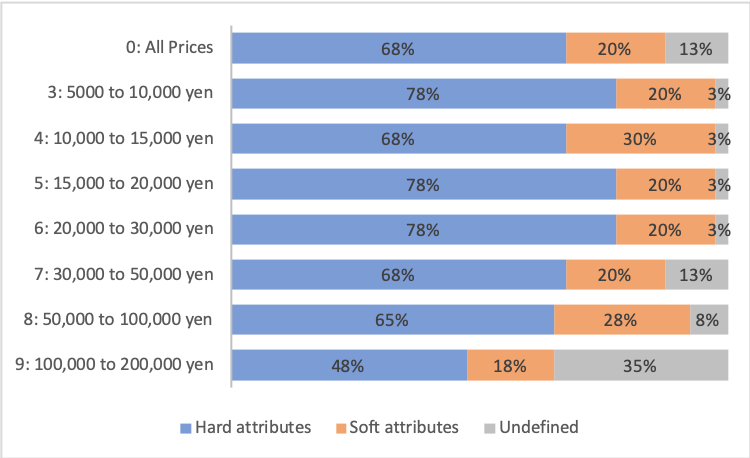
\includegraphics[width=\textwidth]{hard_soft_attr_zh_pos.png}
          \caption{Positive keywords}
      \end{subfigure}
      \begin{subfigure}[b]{0.45\textwidth}
          \includegraphics[width=\textwidth]{hard_soft_attr_zh_neg.png}
          \caption{Negative keywords}
      \end{subfigure}
  \caption{Hard and soft attributes from the top Chinese keywords for all price ranges}
  \label{fig:hard_soft_zh}
  \end{figure}

  % Please add the following required packages to your document preamble:
  % \usepackage{multirow}
  % \usepackage{graphicx}
  % \usepackage[normalem]{ulem}
  % \useunder{\uline}{\ul}{}
  \begin{table}[ht]
    \centering
    \caption{Determination of hard and soft attributes for English keywords. }
    \label{tab:en_hard_soft_keywords}
    \resizebox{0.7\textwidth}{!}{%
    \begin{tabular}{|c|l|l|}
      \hline
      \textbf{Keyword Emotion}                     & \multicolumn{1}{c|}{\textbf{Keyword}} & \multicolumn{1}{c|}{\textbf{Attribute Category}} \\ \hline
      \multirow{18}{*}{\textbf{Positive Keywords}} & good                                  & 25\% hard, 50\% soft, 25\% undefined             \\ \cline{2-3} 
       & great          & 50\% hard, 25\% soft, 25\% undefined \\ \cline{2-3} 
       & staff          & 100\% soft                           \\ \cline{2-3} 
       & clean          & 100\% soft                           \\ \cline{2-3} 
       & location       & 100\% hard                           \\ \cline{2-3} 
       & nice           & 50\% hard, 25\% soft, 25\% undefined \\ \cline{2-3} 
       & excellent      & 25\% hard, 50\% soft, 25\% undefined \\ \cline{2-3} 
       & helpful        & 100\% soft                           \\ \cline{2-3} 
       & comfortable    & 25\% hard, 50\% soft, 25\% undefined \\ \cline{2-3} 
       & shopping       & 100\% hard                           \\ \cline{2-3} 
       & beautiful      & 25\% hard, 75\% soft                 \\ \cline{2-3} 
       & friendly       & 100\% soft                           \\ \cline{2-3} 
       & train          & 100\% hard                           \\ \cline{2-3} 
       & large          & 100\% hard                           \\ \cline{2-3} 
       & free           & 100\% soft                           \\ \cline{2-3} 
       & subway         & 100\% hard                           \\ \cline{2-3} 
       & recommend      & 100\% undefined                      \\ \cline{2-3} 
       & wonderful      & 50\% soft, 50\% undefined            \\ \hline
      \multirow{24}{*}{\textbf{Negative Keywords}} & pricey                                & 100\% soft                                       \\ \cline{2-3} 
       & worst          & 25\% hard, 50\% soft, 25\% undefined \\ \cline{2-3} 
       & dated          & 75\% hard, 25\% undefined            \\ \cline{2-3} 
       & poor           & 100\% soft                           \\ \cline{2-3} 
       & walkway        & 100\% hard                           \\ \cline{2-3} 
       & sense          & 100\% undefined                      \\ \cline{2-3} 
       & unable         & 100\% soft                           \\ \cline{2-3} 
       & disappointing  & 50\% soft, 50\% undefined            \\ \cline{2-3} 
       & minor          & 100\% undefined                      \\ \cline{2-3} 
       & worse          & 100\% undefined                      \\ \cline{2-3} 
       & annoying       & 75\% hard, 25\% undefined            \\ \cline{2-3} 
       & lighting       & 100\% soft                           \\ \cline{2-3} 
       & uncomfortable  & 100\% soft                           \\ \cline{2-3} 
       & carpet         & 100\% soft                           \\ \cline{2-3} 
       & dirty          & 75\% soft, 25\% undefined            \\ \cline{2-3} 
       & cigarette      & 100\% soft                           \\ \cline{2-3} 
       & funny smell    & 100\% soft                           \\ \cline{2-3} 
       & rude           & 100\% soft                           \\ \cline{2-3} 
       & smallest       & 75\% hard, 25\% undefined            \\ \cline{2-3} 
       & mixed          & 100\% undefined                      \\ \cline{2-3} 
       & renovation     & 100\% hard                           \\ \cline{2-3} 
       & paper          & 100\% undefined                      \\ \cline{2-3} 
       & disappointment & 100\% undefined                      \\ \cline{2-3} 
       & outdated       & 75\% hard, 25\% undefined            \\ \hline
      \end{tabular}%
      }
  \end{table}

  \begin{figure}[ht]
      \centering
      \begin{subfigure}[b]{0.45\textwidth}
          \includegraphics[width=\textwidth]{hard_soft_attr_en_pos.png}
          \caption{Positive keywords}
      \end{subfigure}
      \begin{subfigure}[b]{0.45\textwidth}
          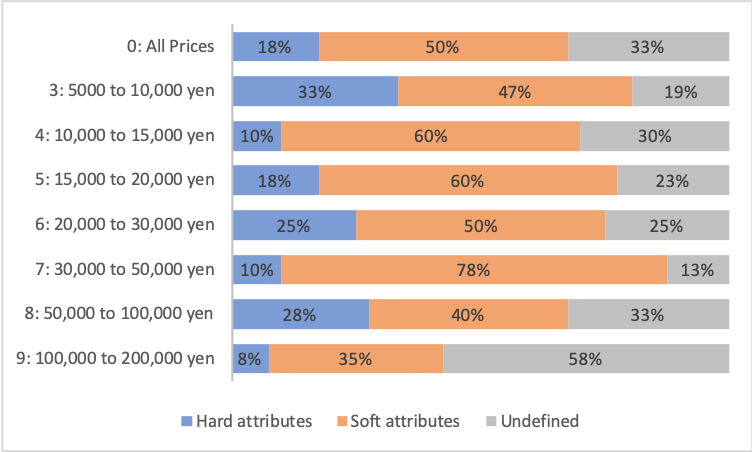
\includegraphics[width=\textwidth]{hard_soft_attr_en_neg.png}
          \caption{Negative keywords}
      \end{subfigure}
  \caption{Hard and soft attributes from the top English keywords for all price ranges}
  \label{fig:hard_soft_en}
  \end{figure}


\section{Results}\label{results}

  \subsection{\DIFdelbegin \DIFdel{Experiment }\DIFdelend \DIFaddbegin \DIFadd{Experimental }\DIFaddend results and \DIFdelbegin \DIFdel{answering }\DIFdelend \DIFaddbegin \DIFadd{answers to }\DIFaddend research questions}

    Our research questions were \DIFdelbegin \DIFdel{about two things. In }\DIFdelend \DIFaddbegin \DIFadd{related to two issues. Based on }\DIFaddend research questions \ref{rsq:hospitality} and \ref{rsq:hospitality_both}, \DIFdelbegin \DIFdel{we decide that }\DIFdelend the objective of this study \DIFdelbegin \DIFdel{to determine }\DIFdelend \DIFaddbegin \DIFadd{was to determine the differences in }\DIFaddend how Chinese and Western tourists \DIFdelbegin \DIFdel{interact with the }\textit{\DIFdel{omotenashi}} %DIFAUXCMD
\DIFdel{culture influenced }\DIFdelend \DIFaddbegin \DIFadd{perceive Japanese hotels, whose }\DIFaddend hospitality and service \DIFdelbegin \DIFdel{in Japan, and how are they different in their perceptions in this matter. 
We observed }\DIFdelend \DIFaddbegin \DIFadd{are influenced by the }\textit{\DIFadd{omotenashi}} \DIFadd{culture. 
}

    \DIFadd{Observing }\DIFaddend the top-ranking positive \DIFdelbegin \DIFdel{factors for Chinese tourists across different price ranges in Table \ref{tab:freq_res_pos} , and specifically the word ``}\begin{CJK}{UTF8}{gbsn}\DIFdel{不错}\end{CJK}\DIFdel{(not bad)'' and its pairings in Table \ref{tab:adj_zh_pos}. From these observations, we can infer }\DIFdelend \DIFaddbegin \DIFadd{keywords in Chinese reviews, as shown in Tables \ref{tab:freq_res_pos} and Table \ref{tab:adj_zh_pos}, it was revealed }\DIFaddend that, while service, cleanliness, and breakfast \DIFdelbegin \DIFdel{are }\DIFdelend \DIFaddbegin \DIFadd{were }\DIFaddend praised in most hotels, \DIFdelbegin \DIFdel{location is usually placed above it in importance on }\DIFdelend \DIFaddbegin \DIFadd{the location was more important when observing }\DIFaddend the pairings. \DIFdelbegin \DIFdel{When we see the rest of the factors }\DIFdelend \DIFaddbegin \DIFadd{Hard attributes were abundant }\DIFaddend lower on the \DIFdelbegin \DIFdel{list, we see that the list is more populated with hard attributes like location and transportation availability across different price ranges. From the negative keyword usages }\DIFdelend \DIFaddbegin \DIFadd{lists. The negative keywords }\DIFaddend in Table \ref{tab:freq_res_neg} \DIFdelbegin \DIFdel{, there are complaints about the }\DIFdelend \DIFaddbegin \DIFadd{indicate that a }\DIFaddend lack of a \DIFdelbegin \DIFdel{Chinese friendly environment . However, most complaints are also }\DIFdelend \DIFaddbegin \DIFadd{Chinese-friendly environment was perceived, although there were more complaints }\DIFaddend about hard attributes such as the building's age and the distance from other convenient spots. \DIFdelbegin \DIFdel{Nevertheless, the most complained about aspect is the price of the hotel. Surprisingly, }\DIFdelend \DIFaddbegin \DIFadd{However, most complaints were about the hotel's price, which included }\DIFaddend all of the price ranges\DIFdelbegin \DIFdel{have this negative keyword at the top of the list, suggesting that it is the main concern to }\DIFdelend \DIFaddbegin \DIFadd{; therefore, the price was the primary concern for }\DIFaddend Chinese customers with different travel purposes.

    On the other hand, the word ``staff'' is the second or third in the lists of satisfaction factors in English-written reviews in all the price ranges. This word is followed by a few other keywords lower in the top 10 list, such as ``helpful'' or ``friendly''. When we look at the pairings of the top-ranked keyword ``good'' in Table \ref{tab:adj_en_pos}, we find that customers mostly praise the location, service, breakfast, or English availability. When we look at the negative keyword ``poor'' and its pairings in Table \ref{tab:adj_en_neg}, we see that it is also service-related concepts that the Western tourists are disappointed with. 
\DIFdelbegin \DIFdel{With these results, we can observe that both Chinese and English-speaking tourists in Japan have different priorities. However, both populations consider the hotel's location and transport availability (subways and trains) nearby as secondary but still essential points in their satisfaction with a hotel. The Chinese customers are primarily satisfied with the room quality in spaciousness and cleanliness and the service of breakfast.
}\DIFdelend 

    \DIFdelbegin \DIFdel{In contrast, the English-speaking customers are easily upset by any lack of cleanliness and smoke smell from cigarettes. Surprisingly, the cigarette smell is an issue even in the middle to high-class hotels above 30,000 yen per night. However, above 50,000 yen per night, this problem seems to disappear from the list of top 10 concerns. Old and dated buildings seem to be a concern for both populations. On the positive side, for all price ranges considered, English-speaking tourists value staff friendliness over room quality when considering their satisfaction. In contrast, Chinese tourists consider location and transportation more often.
}%DIFDELCMD < 

%DIFDELCMD <     %%%
\DIFdel{We also can }\DIFdelend \DIFaddbegin \DIFadd{We can also }\DIFaddend observe some keywords that are not considered by their counterparts. For example, English-speaking customers mentioned tobacco smell in many reviews. However, it was not statistically identified as a problem for their Chinese counterparts. On the other hand, \DIFdelbegin \DIFdel{while it appears }\DIFdelend \DIFaddbegin \DIFadd{although they appear }\DIFaddend in both English and Chinese lists, references to ``\begin{CJK}{UTF8}{gbsn}购物\end{CJK} (shopping)'' are more common in the Chinese lists across hotels of 15,000 yen to 200,000 yen per night. Meanwhile, the term ``shopping'' \DIFdelbegin \DIFdel{only appears in the }\DIFdelend \DIFaddbegin \DIFadd{appeared solely in the top 10 positive keywords list for English speakers who stayed in rooms priced }\DIFaddend 20,000\DIFdelbegin \DIFdel{to }\DIFdelend \DIFaddbegin \DIFadd{–}\DIFaddend 30,000 yen per night\DIFdelbegin \DIFdel{top 10 positive keywords list for English-speakers}\DIFdelend .

    \DIFdelbegin \DIFdel{In our research questions \ref{rsq:hard_soft} and \ref{rsq:hard_soft_diff}, we ponder how customers of both cultural backgrounds evaluate hard and soft attributes of the hotel and how they differ in those evaluations. Here we define hard attributes as those relating to }\DIFdelend \DIFaddbegin \DIFadd{With these results, we can observe that both Chinese and English-speaking tourists in Japan have different priorities. However, both populations consider }\DIFaddend the hotel's \DIFdelbegin \DIFdel{physical, structural, or environmental aspects. These are often impossible or impractical to change by the hotel management and staff, such as facilities, infrastructure, the surroundings, view, or location convenience.
On the other hand, hotel staff and management can change soft attributes , for example, by improving the hotel's services via training or hiring specialized staff, improving the quantity or quality of amenities, bedsheets, or general cleanliness}\DIFdelend \DIFaddbegin \DIFadd{location and transport availability (subways and trains) nearby as secondary but still essential points in their satisfaction with a hotel. The Chinese customers are primarily satisfied with the room quality in spaciousness and cleanliness and the service of breakfast.
}

    \DIFadd{For research questions \ref{rsq:hard_soft} and \ref{rsq:hard_soft_diff}, we considered how customers of both cultural backgrounds evaluated the hard and soft attributes of hotels}\DIFaddend . Our study \DIFdelbegin \DIFdel{found }\DIFdelend \DIFaddbegin \DIFadd{discovered }\DIFaddend that Chinese tourists \DIFdelbegin \DIFdel{are mostly positively reacting more }\DIFdelend \DIFaddbegin \DIFadd{mostly positively react }\DIFaddend to the hotel's hard attributes\DIFdelbegin \DIFdel{. There is a slightly hard leaning (53\%) concern with hard attributes in negative sentences, albeit this is }\DIFdelend \DIFaddbegin \DIFadd{, albeit the negative evaluations are }\DIFaddend more uniform than the positive evaluations\DIFdelbegin \DIFdel{. English-speaking tourists, on }\DIFdelend \DIFaddbegin \DIFadd{, with a tendency of 53 \% towards hard attributes. On }\DIFaddend the other hand, \DIFdelbegin \DIFdel{are both positively and negatively }\DIFdelend \DIFaddbegin \DIFadd{English-speaking tourists were }\DIFaddend more responsive to soft attributes\DIFaddbegin \DIFadd{, either positively or negatively}\DIFaddend . In the case of negative keywords, \DIFdelbegin \DIFdel{English-speaking tourists are overwhelmingly more concerned with }\DIFdelend \DIFaddbegin \DIFadd{they were more concerned about }\DIFaddend the hotel's soft attributes\DIFdelbegin \DIFdel{dissatisfaction somehow}\DIFdelend .

    One factor that both populations \DIFdelbegin \DIFdel{have }\DIFdelend \DIFaddbegin \DIFadd{had }\DIFaddend in common is \DIFaddbegin \DIFadd{that}\DIFaddend , when perceiving the hotel negatively, \DIFaddbegin \DIFadd{the }\DIFaddend ``\begin{CJK}{UTF8}{gbsn}老\end{CJK} (old)\DIFdelbegin \DIFdel{'',``dated'',``outdated'',}\DIFdelend \DIFaddbegin \DIFadd{,'' ``dated,'' ``outdated,'' }\DIFaddend or ``\begin{CJK}{UTF8}{gbsn}陈旧\end{CJK} (obsolete)'' aspects of the room or the hotel \DIFdelbegin \DIFdel{are being criticized across , surprisingly, }\DIFdelend \DIFaddbegin \DIFadd{were surprisingly criticized across }\DIFaddend most price ranges. \DIFdelbegin \DIFdel{This is, however, }\DIFdelend \DIFaddbegin \DIFadd{However, this is }\DIFaddend a hard attribute and is unlikely to change for most hotels.

  \subsection{Chinese tourists\DIFdelbegin \DIFdel{- }\DIFdelend \DIFaddbegin \DIFadd{: }\DIFaddend A big and clean space}\label{disc:zh}

    We found that mainland Chinese tourists \DIFdelbegin \DIFdel{are satisfied mostly by Japanese hotels' }\DIFdelend \DIFaddbegin \DIFadd{were mainly satisfied by }\DIFaddend big and clean spaces \DIFdelbegin \DIFdel{. From the adjectival pairings that we }\DIFdelend \DIFaddbegin \DIFadd{in Japanese hotels. The adjectival pairings }\DIFaddend extracted with dependency parsing and POS tagging \DIFdelbegin \DIFdel{in Table \ref{tab:adj_zh_pos}, we can observe that mostly they mean }\DIFdelend \DIFaddbegin \DIFadd{(Table \ref{tab:adj_zh_pos})  imply }\DIFaddend big and clean rooms. Other mentions \DIFdelbegin \DIFdel{are also }\DIFdelend \DIFaddbegin \DIFadd{included }\DIFaddend big markets nearby or a big bed. \DIFdelbegin \DIFdel{We can observe that across }\DIFdelend \DIFaddbegin \DIFadd{Across }\DIFaddend different price ranges, the usage of the word ``\begin{CJK}{UTF8}{gbsn}大\end{CJK} (big)'' \DIFdelbegin \DIFdel{increases as the hotel increases in price . However, we can see that they still react positively in a significant manner in cheaper hotels. Inspecting }\DIFdelend \DIFaddbegin \DIFadd{increased with the increasing price of the hotel. When inspecting }\DIFaddend closer by taking random samples of the pairs of ``\begin{CJK}{UTF8}{gbsn}大 空间\end{CJK} (big space)'' or ``\begin{CJK}{UTF8}{gbsn}大 面积\end{CJK} (large area)\DIFdelbegin \DIFdel{'',we can see that there are }\DIFdelend \DIFaddbegin \DIFadd{,'' we notice that there were }\DIFaddend also many references to the public bathing facilities in the hotel. \DIFdelbegin \DIFdel{We can also see them mentioned as }\DIFdelend \DIFaddbegin \DIFadd{Such references were also implied by }\DIFaddend a word pairing ``\begin{CJK}{UTF8}{gbsn}棒 温泉\end{CJK} (great hot spring)\DIFdelbegin \DIFdel{''.}\DIFdelend \DIFaddbegin \DIFadd{.'' 
}

    \DIFaddend In Japan, there \DIFdelbegin \DIFdel{is what is called }\DIFdelend \DIFaddbegin \DIFadd{are the so-called }\DIFaddend ``\begin{CJK}{UTF8}{min}銭湯\end{CJK} (\textit{sent\=o})\DIFdelbegin \DIFdel{'',}\DIFdelend \DIFaddbegin \DIFadd{,'' }\DIFaddend which are artificially \DIFdelbegin \DIFdel{made }\DIFdelend \DIFaddbegin \DIFadd{constructed }\DIFaddend public bathing facilities, \DIFdelbegin \DIFdel{on occasions }\DIFdelend including saunas and baths with unique qualities. On the other hand, there are natural hot springs, called ``\begin{CJK}{UTF8}{gbsn}温泉\end{CJK} (\textit{onsen})\DIFdelbegin \DIFdel{''.They can either be bathing in the natural source of the water or using the hot springs }\DIFdelend \DIFaddbegin \DIFadd{.'' However, they are interchangeable if natural hot spring water is used }\DIFaddend in artificially made \DIFaddbegin \DIFadd{tiled }\DIFaddend bath facilities. It is a Japanese custom \DIFdelbegin \DIFdel{and culture }\DIFdelend that all customers \DIFdelbegin \DIFdel{use the facilities after cleaning }\DIFdelend \DIFaddbegin \DIFadd{first clean }\DIFaddend themselves in a shower and \DIFdelbegin \DIFdel{go into the baths without any clothes. It can }\DIFdelend \DIFaddbegin \DIFadd{afterward use the baths nude. It could }\DIFaddend be a cultural shock for many tourists \DIFdelbegin \DIFdel{, but this is }\DIFdelend \DIFaddbegin \DIFadd{but }\DIFaddend a fundamental attraction for many \DIFaddbegin \DIFadd{others}\DIFaddend . 

    \DIFdelbegin \DIFdel{However, }\DIFdelend \DIFaddbegin \DIFadd{Chinese customers are satisfied with }\DIFaddend the size of the room or \DIFdelbegin \DIFdel{the bedis a hard attribute. Without considering rebuilding the hotel}\DIFdelend \DIFaddbegin \DIFadd{bed; however}\DIFaddend , it is not trivial to \DIFdelbegin \DIFdel{improve on. On the other hand}\DIFdelend \DIFaddbegin \DIFadd{change this. In contrast}\DIFaddend , cleanliness is mostly \DIFdelbegin \DIFdel{relating }\DIFdelend \DIFaddbegin \DIFadd{related }\DIFaddend to soft attributes when we observe its adjectival pairings. We can observe pairs such as ``\begin{CJK}{UTF8}{gbsn}干净 房间\end{CJK} (clean room)'' at the top rank of all price ranges \DIFdelbegin \DIFdel{, and then variably }\DIFdelend \DIFaddbegin \DIFadd{and thereupon }\DIFaddend ``\begin{CJK}{UTF8}{gbsn}干净 酒店\end{CJK} (clean hotel)\DIFdelbegin \DIFdel{'',}\DIFdelend \DIFaddbegin \DIFadd{,'' }\DIFaddend ``\begin{CJK}{UTF8}{gbsn}干净 总体\end{CJK} (clean overall)\DIFdelbegin \DIFdel{'',}\DIFdelend \DIFaddbegin \DIFadd{,'' }\DIFaddend ``\begin{CJK}{UTF8}{gbsn}干净 环境\end{CJK} (clean environment)\DIFdelbegin \DIFdel{'',}\DIFdelend \DIFaddbegin \DIFadd{,'' }\DIFaddend and ``\begin{CJK}{UTF8}{gbsn}干净 设施\end{CJK} (clean facilities)\DIFdelbegin \DIFdel{'',}\DIFdelend \DIFaddbegin \DIFadd{,'' }\DIFaddend among other examples. In negative reviews, there \DIFdelbegin \DIFdel{is }\DIFdelend \DIFaddbegin \DIFadd{was }\DIFaddend a mention of criticizing the ``\begin{CJK}{UTF8}{gbsn}一般 卫生\end{CJK} (general hygiene)'' of the hotel, although it \DIFdelbegin \DIFdel{is }\DIFdelend \DIFaddbegin \DIFadd{was }\DIFaddend an uncommon pair. Therefore, we can assert that cleanliness \DIFdelbegin \DIFdel{is }\DIFdelend \DIFaddbegin \DIFadd{was }\DIFaddend an important soft attribute for Chinese customers\DIFdelbegin \DIFdel{and that they are mostly pleased with their expectations being met}\DIFdelend \DIFaddbegin \DIFadd{, and they were mostly pleased when their expectations were fulfilled}\DIFaddend . 

    \DIFdelbegin \DIFdel{One key component we found in Chinese customer satisfaction soft factors is }\DIFdelend \DIFaddbegin \DIFadd{A key soft satisfaction factor was }\DIFaddend the inclusion of breakfast within the hotel. While other food-related words were extracted, most of them were general, \DIFdelbegin \DIFdel{like }\DIFdelend \DIFaddbegin \DIFadd{such as }\DIFaddend ``food'' or ``eating,'' \DIFdelbegin \DIFdel{which were lower ranking}\DIFdelend \DIFaddbegin \DIFadd{and were lower-ranking}\DIFaddend . In contrast, the word ``\begin{CJK}{UTF8}{gbsn}早餐\end{CJK} (breakfast)\DIFdelbegin \DIFdel{'' refers possibly to its inclusion in }\DIFdelend \DIFaddbegin \DIFadd{,'' referring to }\DIFaddend the hotel commodities, was frequently used in positive texts compared to other food-related words \DIFdelbegin \DIFdel{. The word ``}\begin{CJK}{UTF8}{gbsn}\DIFdel{早餐}\end{CJK}\DIFdel{(breakfast)'' is also observed }\DIFdelend across all price ranges, \DIFdelbegin \DIFdel{although }\DIFdelend \DIFaddbegin \DIFadd{albeit }\DIFaddend at different priorities in each of them. \DIFdelbegin \DIFdel{However, we assert that it is }\DIFdelend \DIFaddbegin \DIFadd{For this reason, we regard it as }\DIFaddend an important factor. \DIFdelbegin \DIFdel{Observing word pairs from }\DIFdelend \DIFaddbegin \DIFadd{From the word pairs of }\DIFaddend the positive Chinese keywords in Table \ref{tab:adj_zh_pos}, we can also \DIFdelbegin \DIFdel{see }\DIFdelend \DIFaddbegin \DIFadd{note }\DIFaddend that ``\begin{CJK}{UTF8}{gbsn}不错\end{CJK} (not bad)'' is paired \DIFdelbegin \DIFdel{as }\DIFdelend \DIFaddbegin \DIFadd{with }\DIFaddend ``\begin{CJK}{UTF8}{gbsn}不错 早餐\end{CJK} (nice breakfast)'' in four of the seven price ranges with reviews available as part of the top \DIFdelbegin \DIFdel{4 }\DIFdelend \DIFaddbegin \DIFadd{four }\DIFaddend pairings. It is only slightly lower \DIFdelbegin \DIFdel{on }\DIFdelend \DIFaddbegin \DIFadd{in }\DIFaddend other categories, although it is not \DIFdelbegin \DIFdel{shown on }\DIFdelend \DIFaddbegin \DIFadd{depicted in }\DIFaddend the table. Thus\DIFaddbegin \DIFadd{, }\DIFaddend we consider that a recommended strategy for hotel management is to invest in the inclusion or \DIFdelbegin \DIFdel{betterment }\DIFdelend \DIFaddbegin \DIFadd{improvement }\DIFaddend of hotel breakfast to increase good reviews.

  \subsection{Western tourists\DIFdelbegin \DIFdel{- }\DIFdelend \DIFaddbegin \DIFadd{: }\DIFaddend A friendly face \DIFdelbegin \DIFdel{, }\DIFdelend and absolutely clean}\label{disc:en}

    From the satisfaction factors of English-speaking tourists, we \DIFdelbegin \DIFdel{can see that }\DIFdelend \DIFaddbegin \DIFadd{observed }\DIFaddend at least three words \DIFdelbegin \DIFdel{relate directly }\DIFdelend \DIFaddbegin \DIFadd{were related }\DIFaddend to staff friendliness and services \DIFdelbegin \DIFdel{, being ``staff'',``helpful}\DIFdelend \DIFaddbegin \DIFadd{in the general database: ``staff,'' ``helpful,}\DIFaddend '' and ``friendliness\DIFdelbegin \DIFdel{'' in the general database.}\DIFdelend \DIFaddbegin \DIFadd{.'' }\DIFaddend The word ``staff'' is the \DIFdelbegin \DIFdel{second most frequently used word }\DIFdelend \DIFaddbegin \DIFadd{highest-ranked of these three, ranking second }\DIFaddend for satisfied customers across most price ranges \DIFdelbegin \DIFdel{, }\DIFdelend and only third in one of them. \DIFdelbegin \DIFdel{Adding to that, ``helpful'' and ``friendly'' follow it lower in the list in most price ranges. }\DIFdelend The word ``good'' \DIFdelbegin \DIFdel{is mostly about }\DIFdelend \DIFaddbegin \DIFadd{mainly refers to }\DIFaddend the location, \DIFdelbegin \DIFdel{the }\DIFdelend service, breakfast, or English availability in Table \ref{tab:adj_en_pos}. \DIFdelbegin \DIFdel{Like }\DIFdelend \DIFaddbegin \DIFadd{Similar to }\DIFaddend Chinese customers, Western customers also \DIFdelbegin \DIFdel{seem }\DIFdelend \DIFaddbegin \DIFadd{seemed }\DIFaddend to enjoy the included breakfasts regarding their satisfaction keyword pairings. However, the \DIFaddbegin \DIFadd{relevant }\DIFaddend word does not appear \DIFdelbegin \DIFdel{directly }\DIFdelend in the top 10 list \DIFdelbegin \DIFdel{as in }\DIFdelend \DIFaddbegin \DIFadd{directly, in contrast to }\DIFaddend their Chinese counterparts. The words ``helpful'' and ``friendly'' are mostly paired with ``staff\DIFdelbegin \DIFdel{'',``concierge'',``desk'',}\DIFdelend \DIFaddbegin \DIFadd{,'' ``concierge,'' ``desk,'' }\DIFaddend and ``service\DIFdelbegin \DIFdel{''.When we look at }\DIFdelend \DIFaddbegin \DIFadd{.'' By considering }\DIFaddend the negative keyword \DIFdelbegin \DIFdel{‘poor’ }\DIFdelend \DIFaddbegin \DIFadd{``poor'' }\DIFaddend and its pairings in Table \ref{tab:adj_en_neg}, we \DIFdelbegin \DIFdel{see that it is also }\DIFdelend \DIFaddbegin \DIFadd{realized once again that Western tourists were disappointed with }\DIFaddend service-related \DIFdelbegin \DIFdel{concepts that the Western tourists are disappointed with when they react }\DIFdelend \DIFaddbegin \DIFadd{concepts and reacted }\DIFaddend negatively.

    Another soft attribute that is high on the list for most of the price ranges is the word ``clean''\DIFdelbegin \DIFdel{. Since it is an adjective, we have explored the word pairingsas well. Customers are mostly praising }\DIFdelend \DIFaddbegin \DIFadd{, so we examined its word pairings. Customers largely praised }\DIFaddend ``clean rooms'' and ``clean bathrooms'' \DIFdelbegin \DIFdel{, while also referring }\DIFdelend \DIFaddbegin \DIFadd{and also referred }\DIFaddend to the hotel in general. \DIFdelbegin \DIFdel{It seems that when }\DIFdelend \DIFaddbegin \DIFadd{When }\DIFaddend observing the negative keyword frequencies for \DIFdelbegin \DIFdel{English-speakers}\DIFdelend \DIFaddbegin \DIFadd{English speakers}\DIFaddend , we can find words such as ``dirty'' \DIFdelbegin \DIFdel{, }\DIFdelend \DIFaddbegin \DIFadd{and }\DIFaddend ``carpet'' \DIFdelbegin \DIFdel{, and from the word pairings }\DIFdelend \DIFaddbegin \DIFadd{as well as word pairings such as }\DIFaddend ``dirty carpet\DIFdelbegin \DIFdel{'',}\DIFdelend \DIFaddbegin \DIFadd{,'' }\DIFaddend ``dirty room\DIFdelbegin \DIFdel{'',}\DIFdelend \DIFaddbegin \DIFadd{,'' }\DIFaddend and ``dirty bathroom\DIFdelbegin \DIFdel{''.}\DIFdelend \DIFaddbegin \DIFadd{.'' }\DIFaddend Along with complaints about off-putting smells, we \DIFdelbegin \DIFdel{can }\DIFdelend \DIFaddbegin \DIFadd{could }\DIFaddend conclude that Western tourists \DIFdelbegin \DIFdel{have }\DIFdelend \DIFaddbegin \DIFadd{had }\DIFaddend high expectations about cleanliness when traveling in Japan.

    An interesting detail of the keyword ranking is that the word ``comfortable'' \DIFdelbegin \DIFdel{is }\DIFdelend \DIFaddbegin \DIFadd{was }\DIFaddend high on the satisfaction factors\DIFaddbegin \DIFadd{, }\DIFaddend and ``uncomfortable'' \DIFaddbegin \DIFadd{was }\DIFaddend high on the dissatisfaction factors. The words \DIFdelbegin \DIFdel{are }\DIFdelend \DIFaddbegin \DIFadd{were }\DIFaddend paired with nouns \DIFdelbegin \DIFdel{like ``bed'',or ``room'',``pillow'' or ``mattress'',generally referring }\DIFdelend \DIFaddbegin \DIFadd{such as ``bed,'' ``room,'' ``pillow,'' and ``mattress,'' when they generally referred }\DIFaddend to their sleep conditions in the hotel.
    It seems that Western tourists \DIFdelbegin \DIFdel{are highly sensitive to comfort levels in the hotelsand whether it reaches }\DIFdelend \DIFaddbegin \DIFadd{were particularly sensitive about the hotels’ comfort levels and whether they reached }\DIFaddend their expectations. The ranking for the negative keyword ``uncomfortable'' is similar across most price ranges \DIFdelbegin \DIFdel{, }\DIFdelend except the two most expensive ones, where this keyword disappears from the top 10 list.

    \DIFdelbegin \DIFdel{While less high }\DIFdelend \DIFaddbegin \DIFadd{Albeit lower }\DIFaddend in priority, the price range of 15,000 to 20,000 yen hotels also \DIFdelbegin \DIFdel{mentions }\DIFdelend \DIFaddbegin \DIFadd{includes }\DIFaddend ``free'' as one of the top 10 positive keywords, \DIFdelbegin \DIFdel{paired mostly with ``wifi''.}\DIFdelend \DIFaddbegin \DIFadd{mainly paired with ``Wi-Fi.'' }\DIFaddend This price range \DIFdelbegin \DIFdel{is mostly for }\DIFdelend \DIFaddbegin \DIFadd{corresponds to }\DIFaddend business hotels, where \DIFdelbegin \DIFdel{we infer users would be expecting }\DIFdelend \DIFaddbegin \DIFadd{users would expect }\DIFaddend this feature the most. 
\DIFdelbegin \DIFdel{Western tourists are highly sensitive to comfort levels in the hotels and whether it reaches their expectations.
}\DIFdelend 

  \subsection{Tobacco, \DIFdelbegin \DIFdel{what's that }\DIFdelend \DIFaddbegin \DIFadd{an unpleasant }\DIFaddend smell \DIFdelbegin \DIFdel{?}\DIFdelend \DIFaddbegin \DIFadd{in the room}\DIFaddend }\label{disc:tobacco}

    A concern for Western tourists was \DIFaddbegin \DIFadd{uncleanliness and }\DIFaddend the smell of \DIFdelbegin \DIFdel{tobacco }\DIFdelend \DIFaddbegin \DIFadd{cigarettes }\DIFaddend in their room, which can be \DIFdelbegin \DIFdel{considered a soft attribute. Tobacco was found not only as a standalone word }\DIFdelend \DIFaddbegin \DIFadd{regarded as soft attributes. Cigarette smell was an issue even in the middle- and high-class hotels, of which the rooms were priced at more than 30,000 yen per night. For hotels with rooms priced above 50,000 yen per night, however, this problem seemed to disappear from the list of top 10 concerns. Tobacco was referenced singularly as }\DIFaddend ``cigarette'', but also \DIFdelbegin \DIFdel{as }\DIFdelend \DIFaddbegin \DIFadd{in }\DIFaddend word pairs in Table \ref{tab:adj_en_neg} \DIFdelbegin \DIFdel{. We can find other related word pairs such }\DIFdelend as ``funny smell\DIFdelbegin \DIFdel{''.Upon manual inspection of }\DIFdelend \DIFaddbegin \DIFadd{.'' By manually inspecting }\DIFaddend a sample of reviews with this keyword, we \DIFdelbegin \DIFdel{found }\DIFdelend \DIFaddbegin \DIFadd{noticed }\DIFaddend that the room was often advertised as non-smoking\DIFdelbegin \DIFdel{, yet, }\DIFdelend \DIFaddbegin \DIFadd{; however, }\DIFaddend the smell permeated the room and curtains. Another common complaint was that there were no \DIFdelbegin \DIFdel{non-smoking facilities availableat all in the first place}\DIFdelend \DIFaddbegin \DIFadd{nonsmoking facilities available}\DIFaddend . The smell of smoke can completely ruin some customers’ stay\DIFdelbegin \DIFdel{and give a bad impression to review writers, }\DIFdelend \DIFaddbegin \DIFadd{, leading to bad reviews, thereby }\DIFaddend lowering the number of future customers.

    \DIFdelbegin \DIFdel{However, in comparison, Chinese customers seem }\DIFdelend \DIFaddbegin \DIFadd{In contrast, Chinese customers seemed }\DIFaddend not to be bothered by this\DIFdelbegin \DIFdel{at all. We consulted studies involving the use of tobacco in different countries. Previous research states }\DIFdelend \DIFaddbegin \DIFadd{. Previous research has stated }\DIFaddend that 49\DIFdelbegin \DIFdel{- }\DIFdelend \DIFaddbegin \DIFadd{–}\DIFaddend 60 \% of Chinese men (and 2.0\DIFdelbegin \DIFdel{- }\DIFdelend \DIFaddbegin \DIFadd{–}\DIFaddend 2.8 \% of women) currently smoke or \DIFdelbegin \DIFdel{have smoked before}\DIFdelend \DIFaddbegin \DIFadd{smoked in the past}\DIFaddend . This was \DIFdelbegin \DIFdel{taken }\DIFdelend \DIFaddbegin \DIFadd{derived }\DIFaddend from a sample of 170,000 Chinese adults in \DIFdelbegin \DIFdel{2013-2014}\DIFdelend \DIFaddbegin \DIFadd{2013–2014}\DIFaddend , which is high compared to many English-speaking countries \cite[][]{zhang2019tobacco,who2015tobacco}.

    Japan has a polarized view on the topic of smoking. \DIFdelbegin \DIFdel{Despite being }\DIFdelend \DIFaddbegin \DIFadd{Although it has }\DIFaddend one of the world’s largest tobacco markets, \DIFdelbegin \DIFdel{its }\DIFdelend \DIFaddbegin \DIFadd{tobacco }\DIFaddend use has decreased in recent years. Smoking in public spaces is prohibited in some wards of Tokyo (namely Chiyoda, Shinjuku, and Shibuya). However, it is generally only \DIFdelbegin \DIFdel{urged }\DIFdelend \DIFaddbegin \DIFadd{suggested }\DIFaddend and not mandatory to \DIFdelbegin \DIFdel{have }\DIFdelend \DIFaddbegin \DIFadd{lift }\DIFaddend smoking restrictions in restaurants, bars, hotels, and public areas. \DIFdelbegin \DIFdel{However, many }\DIFdelend \DIFaddbegin \DIFadd{Many }\DIFaddend places have designated smoking rooms \DIFdelbegin \DIFdel{are available }\DIFdelend to keep the smoke in an enclosed area and avoid bothering others.
\DIFdelbegin \DIFdel{Despite this}\DIFdelend \DIFaddbegin 

    \DIFadd{Nevertheless}\DIFaddend , businesses, especially those who cater to certain customers, \DIFdelbegin \DIFdel{will generally be discouraged from having }\DIFdelend \DIFaddbegin \DIFadd{are generally discouraged by }\DIFaddend smoking restrictions if they want to \DIFdelbegin \DIFdel{keep }\DIFdelend \DIFaddbegin \DIFadd{maintain }\DIFaddend their clientele. \DIFdelbegin \DIFdel{If Japanese hotels want to }\DIFdelend \DIFaddbegin \DIFadd{To }\DIFaddend cater to all kinds of customers, \DIFaddbegin \DIFadd{including }\DIFaddend Western and Asian\DIFdelbegin \DIFdel{alike, they }\DIFdelend \DIFaddbegin \DIFadd{, Japanese hotels }\DIFaddend must provide spaces without tobacco smell. \DIFdelbegin \DIFdel{After all, even if it }\DIFdelend \DIFaddbegin \DIFadd{Even if the smoke }\DIFaddend does not bother a few customers, the lack of \DIFdelbegin \DIFdel{smell would }\DIFdelend \DIFaddbegin \DIFadd{such a smell will }\DIFaddend make it an appropriate space for all customers.

  \subsection{Location, location, location}\label{disc:location}

    The hotel's location, closeness to the subway and public \DIFdelbegin \DIFdel{transport, and nearby shops' availability were observed }\DIFdelend \DIFaddbegin \DIFadd{transportation, and availability of nearby shops proved }\DIFaddend to be of importance to both Chinese and English-speaking tourists. In positive word pairings \DIFaddbegin \DIFadd{in }\DIFaddend Tables \ref{tab:adj_zh_pos} and \ref{tab:adj_en_pos}, we can find pairs such as ``\begin{CJK}{UTF8}{gbsn}不错 位置\end{CJK} (nice location)\DIFdelbegin \DIFdel{'',}\DIFdelend \DIFaddbegin \DIFadd{,'' }\DIFaddend ``\begin{CJK}{UTF8}{gbsn}近 地铁站\end{CJK} (near subway station)\DIFdelbegin \DIFdel{'',}\DIFdelend \DIFaddbegin \DIFadd{,'' }\DIFaddend ``\begin{CJK}{UTF8}{gbsn}近 地铁\end{CJK} (near subway)'' in Chinese texts and ``good location\DIFdelbegin \DIFdel{'',}\DIFdelend \DIFaddbegin \DIFadd{,'' }\DIFaddend ``great location\DIFdelbegin \DIFdel{'',}\DIFdelend \DIFaddbegin \DIFadd{,'' }\DIFaddend and ``great view'' \DIFdelbegin \DIFdel{, }\DIFdelend as well as single keywords ``location'' and ``shopping'' for \DIFdelbegin \DIFdel{English-speakers}\DIFdelend \DIFaddbegin \DIFadd{English speakers}\DIFaddend , and ``\begin{CJK}{UTF8}{gbsn}交通\end{CJK} (traffic)\DIFdelbegin \DIFdel{'',}\DIFdelend \DIFaddbegin \DIFadd{,'' }\DIFaddend ``\begin{CJK}{UTF8}{gbsn}购物\end{CJK} (shopping)\DIFdelbegin \DIFdel{'',}\DIFdelend \DIFaddbegin \DIFadd{,'' }\DIFaddend ``\begin{CJK}{UTF8}{gbsn}地铁\end{CJK} (subway)\DIFdelbegin \DIFdel{'',}\DIFdelend \DIFaddbegin \DIFadd{,'' }\DIFaddend and ``\begin{CJK}{UTF8}{gbsn}环境\end{CJK} (environment or surroundings)'' for Chinese speakers. All of these keywords and their location in each population's priorities across the price ranges \DIFdelbegin \DIFdel{signal that while it was not the priority for either of them, the }\DIFdelend \DIFaddbegin \DIFadd{signify that the }\DIFaddend hotel's location \DIFdelbegin \DIFdel{is }\DIFdelend \DIFaddbegin \DIFadd{was }\DIFaddend a secondary but still important point \DIFdelbegin \DIFdel{in the hotel's }\DIFdelend \DIFaddbegin \DIFadd{for their }\DIFaddend satisfaction. However, since this is a hard attribute, \DIFdelbegin \DIFdel{unchangeable to the hotel's management, }\DIFdelend it is not often considered in the literature. \DIFdelbegin \DIFdel{Upon inspection of }\DIFdelend \DIFaddbegin \DIFadd{By examining }\DIFaddend examples from the data, we \DIFdelbegin \DIFdel{found }\DIFdelend \DIFaddbegin \DIFadd{recognized }\DIFaddend that most customers were satisfied if the hotel was near \DIFdelbegin \DIFdel{to }\DIFdelend at least two \DIFdelbegin \DIFdel{other subjects}\DIFdelend \DIFaddbegin \DIFadd{of the following facilities}\DIFaddend : subway, train, and convenience stores. 

    Japan is a country with a peculiar public \DIFdelbegin \DIFdel{transport system. The rush hourmakes for a subway filled to the brim with people in suits making their commute}\DIFdelend \DIFaddbegin \DIFadd{transportation system. During rush hour, the subway is crowded with commuters}\DIFaddend , and trains and subway stations \DIFdelbegin \DIFdel{in Tokyo }\DIFdelend create a confusing public \DIFdelbegin \DIFdel{transport }\DIFdelend \DIFaddbegin \DIFadd{transportation }\DIFaddend map for a visitor \DIFaddbegin \DIFadd{in Tokyo}\DIFaddend . Buses are also available, \DIFdelbegin \DIFdel{although }\DIFdelend \DIFaddbegin \DIFadd{albeit }\DIFaddend less used than \DIFdelbegin \DIFdel{the }\DIFdelend rail systems in \DIFdelbegin \DIFdel{the big }\DIFdelend \DIFaddbegin \DIFadd{metropolitan }\DIFaddend cities. These three \DIFdelbegin \DIFdel{are unusually }\DIFdelend \DIFaddbegin \DIFadd{means of transportation are usually }\DIFaddend affordable in price. \DIFdelbegin \DIFdel{Then there are the more expensive transports}\DIFdelend \DIFaddbegin \DIFadd{There are more expensive means}\DIFaddend , such as the bullet train \textit{shinkansen} for traveling across the country \DIFdelbegin \DIFdel{, }\DIFdelend and taxis. \DIFdelbegin \DIFdel{Taxis in Japan are a luxury }\DIFdelend \DIFaddbegin \DIFadd{The latter is a luxury in Japan }\DIFaddend compared to other countries. In \DIFdelbegin \DIFdel{less developed countries, a taxi is the cheap method of transport of choice. In }\DIFdelend Japan, taxis \DIFdelbegin \DIFdel{are made to }\DIFdelend provide a high-quality experience with a matching price. \DIFdelbegin \DIFdel{This means that for tourists}\DIFdelend \DIFaddbegin \DIFadd{Therefore, for people under a budget}\DIFaddend , subway availability and maps or GPS applications\DIFdelbegin \DIFdel{and }\DIFdelend \DIFaddbegin \DIFadd{, as well as }\DIFaddend a plan to travel the city\DIFaddbegin \DIFadd{, }\DIFaddend are of utmost necessity \DIFaddbegin \DIFadd{for tourists, using taxis only as a last resort}\DIFaddend . 

    Japanese convenience stores \DIFdelbegin \DIFdel{, on the other hand, }\DIFdelend are also famous worldwide \DIFdelbegin \DIFdel{. Japanese convenience stores are a haven for the traveler in need. It offers anything}\DIFdelend \DIFaddbegin \DIFadd{because they offer a wide range of services and products}\DIFaddend , from drinks and snacks to full meals, copy and scanning machines, alcohol, cleaning supplies, personal hygiene items, underwear, towels, \DIFdelbegin \DIFdel{international ATMs, among other things}\DIFdelend \DIFaddbegin \DIFadd{and international ATMs}\DIFaddend . If some trouble \DIFdelbegin \DIFdel{occurred}\DIFdelend \DIFaddbegin \DIFadd{occurs}\DIFaddend , or a traveler forgot to pack a particular item, it is \DIFdelbegin \DIFdel{almost sure }\DIFdelend \DIFaddbegin \DIFadd{most certain }\DIFaddend that they can find it. 

    Therefore, considering that both \DIFdelbegin \DIFdel{transport }\DIFdelend \DIFaddbegin \DIFadd{transportation }\DIFaddend systems and nearby shops are points of interest for Chinese and Western tourists, \DIFdelbegin \DIFdel{Japanese hotels have to carefully choose their location from the moment they are constructed. While not a top priority, this is a universal factor for both customer groups, and it can be an instant way to generate positive reviews}\DIFdelend \DIFaddbegin \DIFadd{and perhaps offering guide maps and information about these as an appeal point could result in greater satisfaction}\DIFaddend .

\section{Discussion}\label{discussion}

  \DIFdelbegin \DIFdel{Below we explore the possible interactions with Japanese hospitality, the differences between Chinese and Western tourists, the possible cause for them, how they vary across different price ranges, and what they imply for the industry. We also discuss the differences between the hotel's hard and soft attributes and how they contribute to customers' satisfaction.
}%DIFDELCMD < 

%DIFDELCMD <   %%%
\DIFdelend \subsection{Western and Chinese tourists in the Japanese hospitality environment}\label{disc:omotenashi}

    To \DIFdelbegin \DIFdel{this day, scholars continue to correct }\DIFdelend \DIFaddbegin \DIFadd{date, scholars have been correcting }\DIFaddend our historical bias towards the \DIFdelbegin \DIFdel{west}\DIFdelend \DIFaddbegin \DIFadd{West}\DIFaddend . Studies have determined that different cultural backgrounds lead to different expectations, which \DIFdelbegin \DIFdel{influences }\DIFdelend \DIFaddbegin \DIFadd{influence }\DIFaddend tourists' satisfaction. \DIFdelbegin \DIFdel{Meaning}\DIFdelend \DIFaddbegin \DIFadd{In other words}\DIFaddend , tourists of a particular culture \DIFdelbegin \DIFdel{will }\DIFdelend have different leading satisfaction factors across different destinations. However, Japan presents a particular environment\DIFdelbegin \DIFdel{. The }\DIFdelend \DIFaddbegin \DIFadd{; the }\DIFaddend spirit of hospitality and service, \textit{omotenashi}, \DIFdelbegin \DIFdel{excels and is considered }\DIFdelend \DIFaddbegin \DIFadd{which is considered to be of }\DIFaddend the highest standard across the world. \DIFdelbegin \DIFdel{Can }\DIFdelend \DIFaddbegin \DIFadd{Our study explores whether }\DIFaddend such an environment \DIFaddbegin \DIFadd{can }\DIFaddend affect different cultures equally \DIFdelbegin \DIFdel{? Or is it only attractive }\DIFdelend \DIFaddbegin \DIFadd{or whether it is attractive only }\DIFaddend to certain cultures\DIFdelbegin \DIFdel{? Our study brings light to these questions}\DIFdelend .

    Our results indicate that \DIFdelbegin \DIFdel{out of the two, }\DIFdelend Western tourists are \DIFdelbegin \DIFdel{the most }\DIFdelend \DIFaddbegin \DIFadd{more }\DIFaddend satisfied with soft attributes \DIFdelbegin \DIFdel{, such as friendly and helpful staff in Japan}\DIFdelend \DIFaddbegin \DIFadd{than Chinese tourists}\DIFaddend . As explained earlier in this paper, Japan is \DIFdelbegin \DIFdel{famous }\DIFdelend \DIFaddbegin \DIFadd{well known }\DIFaddend for its customer service\DIFdelbegin \DIFdel{all over the world}\DIFdelend . Respectful language and bowing are not exclusive to \DIFdelbegin \DIFdel{high priced }\DIFdelend \DIFaddbegin \DIFadd{high-priced }\DIFaddend hotels or businesses\DIFdelbegin \DIFdel{. These can even be found }\DIFdelend \DIFaddbegin \DIFadd{; these are met }\DIFaddend in convenience stores \DIFdelbegin \DIFdel{. The level of hospitality in even the cheapest of convenience stores }\DIFdelend \DIFaddbegin \DIFadd{as well. Even in the cheapest convenience store, the level of hospitality }\DIFaddend is starkly different from \DIFdelbegin \DIFdel{Westerner experiences. While it could be a culture shock to some, it is mostly seen positively. After all, the Japanese staff respectfully treats all customers. However, for some customers, this could be the best way they have been treated until that moment. Now, in higher priced }\DIFdelend \DIFaddbegin \DIFadd{Western culture and perhaps unexpected. In higher-priced }\DIFaddend hotels, the adjectives used to praise the service \DIFdelbegin \DIFdel{go }\DIFdelend \DIFaddbegin \DIFadd{ranged }\DIFaddend from normal descriptors like ``good'' to higher levels of praise like ``wonderful staff\DIFdelbegin \DIFdel{'',}\DIFdelend \DIFaddbegin \DIFadd{,'' }\DIFaddend ``wonderful experience\DIFdelbegin \DIFdel{'',}\DIFdelend \DIFaddbegin \DIFadd{,'' }\DIFaddend ``excellent service\DIFdelbegin \DIFdel{'',}\DIFdelend \DIFaddbegin \DIFadd{,'' }\DIFaddend and ``excellent staff\DIFdelbegin \DIFdel{''.We can also see that }\DIFdelend \DIFaddbegin \DIFadd{.'' Furthermore, }\DIFaddend \cite{kozak2002} and \cite{shanka2004} have also \DIFdelbegin \DIFdel{found }\DIFdelend \DIFaddbegin \DIFadd{proven }\DIFaddend that hospitality and staff friendliness \DIFdelbegin \DIFdel{is a vital determinant in }\DIFdelend \DIFaddbegin \DIFadd{are two determinants of }\DIFaddend Western tourists' satisfaction.

    However, \DIFdelbegin \DIFdel{we can see from }\DIFdelend the negative English keywords \DIFdelbegin \DIFdel{that a big }\DIFdelend \DIFaddbegin \DIFadd{indicate that a large }\DIFaddend part of the dissatisfaction with Japanese hotels \DIFdelbegin \DIFdel{stems }\DIFdelend \DIFaddbegin \DIFadd{stemmed }\DIFaddend from a lack of hygiene and room cleanliness. Although Chinese customers \DIFdelbegin \DIFdel{only had }\DIFdelend \DIFaddbegin \DIFadd{had solely }\DIFaddend positive keywords about cleanliness, English-speaking customers \DIFdelbegin \DIFdel{have found }\DIFdelend \DIFaddbegin \DIFadd{deemed }\DIFaddend many places unacceptable to their standards\DIFdelbegin \DIFdel{. This is particularly true at hotels }\DIFdelend \DIFaddbegin \DIFadd{, particularly hotels with rooms priced }\DIFaddend below 50,000 yen per night. The most common complaint regarding cleanliness was about the carpet, followed by complaints about cigarette \DIFdelbegin \DIFdel{stench and general dirtiness}\DIFdelend \DIFaddbegin \DIFadd{smell and lack of general hygiene}\DIFaddend . \cite{kozak2002} also \DIFdelbegin \DIFdel{found }\DIFdelend \DIFaddbegin \DIFadd{proved }\DIFaddend that hygiene and cleanliness were essential satisfaction determinants for Western tourists. However, in the previous literature, this was linked merely to satisfaction. In \DIFdelbegin \DIFdel{comparison}\DIFdelend \DIFaddbegin \DIFadd{contrast}\DIFaddend , our research \DIFdelbegin \DIFdel{uncovered that words relating to cleanliness are }\DIFdelend \DIFaddbegin \DIFadd{revealed that words related to cleanliness were }\DIFaddend mostly linked to dissatisfaction. \DIFdelbegin \DIFdel{Westerners could be said to have }\DIFdelend \DIFaddbegin \DIFadd{We could assert that Westerners had }\DIFaddend a high standard of room cleanliness \DIFdelbegin \DIFdel{when }\DIFdelend compared to their Chinese counterparts.

    According to previous research, \DIFdelbegin \DIFdel{we can see that }\DIFdelend Western tourists are already inclined to appreciate hospitality for their satisfaction. When presented with Japanese hospitality, this expectation is met and overcome. In contrast, \DIFdelbegin \DIFdel{we can see from our resultsthat Chinese tourists had less focus on }\DIFdelend \DIFaddbegin \DIFadd{according to our results, Chinese tourists were more concerned about room quality rather than }\DIFaddend hospitality, staff, or service\DIFdelbegin \DIFdel{and were more concerned with room quality}\DIFdelend . However, when analyzing the word pairs for ``\begin{CJK}{UTF8}{gbsn}不错\end{CJK} (not bad)'' and \DIFdelbegin \DIFdel{for }\DIFdelend ``\begin{CJK}{UTF8}{gbsn}棒\end{CJK} (great)\DIFdelbegin \DIFdel{'',}\DIFdelend \DIFaddbegin \DIFadd{,'' }\DIFaddend we can see that they \DIFdelbegin \DIFdel{do }\DIFdelend praise staff, service\DIFaddbegin \DIFadd{, }\DIFaddend and breakfast. \DIFdelbegin \DIFdel{Observing }\DIFdelend \DIFaddbegin \DIFadd{By observing }\DIFaddend the percentage of hard to soft attributes in Figure \ref{fig:hard_soft_zh}, however, we \DIFdelbegin \DIFdel{know }\DIFdelend \DIFaddbegin \DIFadd{discover }\DIFaddend that Chinese customers \DIFdelbegin \DIFdel{are satisfied more }\DIFdelend \DIFaddbegin \DIFadd{were more satisfied }\DIFaddend with hard attributes \DIFdelbegin \DIFdel{, compared to the Western touristswho seem }\DIFdelend \DIFaddbegin \DIFadd{compared }\DIFaddend to \DIFaddbegin \DIFadd{Western tourists, who seemed to }\DIFaddend be meeting more than their expectations.

    It could be \DIFaddbegin \DIFadd{considered }\DIFaddend that Chinese culture does not expect high-level service initially. When an expectation that is not held is met, the satisfaction \DIFdelbegin \DIFdel{that stems from this }\DIFdelend \DIFaddbegin \DIFadd{derived }\DIFaddend is less than \DIFaddbegin \DIFadd{that }\DIFaddend if it was expected. \DIFdelbegin \DIFdel{On the other hand, we have the phenomenon of }\DIFdelend \DIFaddbegin \DIFadd{In contrast, some tourists report }\DIFaddend a ``nice surprise'': \DIFdelbegin \DIFdel{When }\DIFdelend \DIFaddbegin \DIFadd{when }\DIFaddend an unknown need is unexpectedly met, there is more satisfaction. It is necessary to note the difference between these two \DIFdelbegin \DIFdel{phenomenons}\DIFdelend \DIFaddbegin \DIFadd{reactions}\DIFaddend . The ``nice surprise'' \DIFaddbegin \DIFadd{reaction }\DIFaddend fulfills a need unexpectedly. Perhaps the hospitality grade in Japan does not fulfill a \DIFdelbegin \DIFdel{high enough need }\DIFdelend \DIFaddbegin \DIFadd{need high enough }\DIFaddend for the Chinese population, \DIFaddbegin \DIFadd{thereby }\DIFaddend resulting in less satisfaction. For greater satisfaction, \DIFdelbegin \DIFdel{the existence of a need being metis necessary}\DIFdelend \DIFaddbegin \DIFadd{a need must be met}\DIFaddend . However, the word ``not bad'' is at the top of the list \DIFdelbegin \DIFdel{at }\DIFdelend \DIFaddbegin \DIFadd{in }\DIFaddend most price ranges, and one of the uses is related to service. Thus, we cannot \DIFdelbegin \DIFdel{say that they are }\DIFdelend \DIFaddbegin \DIFadd{conclude that they were }\DIFaddend not satisfied with \DIFdelbegin \DIFdel{this matter. Rather, they hold }\DIFdelend \DIFaddbegin \DIFadd{the service. Instead, they held }\DIFaddend other factors at a higher priority\DIFdelbegin \DIFdel{, considering }\DIFdelend \DIFaddbegin \DIFadd{; thus, }\DIFaddend the keyword frequency \DIFdelbegin \DIFdel{is }\DIFdelend \DIFaddbegin \DIFadd{was }\DIFaddend higher for other pairings.

    Another possibility \DIFdelbegin \DIFdel{presents itself }\DIFdelend \DIFaddbegin \DIFadd{occurs }\DIFaddend when we observe the Chinese tourists’ dissatisfaction factors. Chinese tourists may have expectations about \DIFdelbegin \DIFdel{the Chinese visitors' }\DIFdelend \DIFaddbegin \DIFadd{their }\DIFaddend treatment that are not being met, even in this \DIFdelbegin \DIFdel{high standard }\DIFdelend \DIFaddbegin \DIFadd{high-standard }\DIFaddend hospitality environment. \DIFdelbegin \DIFdel{Japan is known worldwide for their hospitality, but they are also known historically to be monolingual and have }\DIFdelend \DIFaddbegin \DIFadd{This could be because Japan is monolingual and has }\DIFaddend a relatively large language barrier \DIFaddbegin \DIFadd{to tourists }\DIFaddend \cite[][]{heinrich2012making,coulmas2002japan}. While the Japanese effort to accommodate English speakers is slowly \DIFdelbegin \DIFdel{taking shape, }\DIFdelend \DIFaddbegin \DIFadd{developing, efforts for }\DIFaddend Chinese accommodations can be lagging. Chinese language pamphlets \DIFdelbegin \DIFdel{, }\DIFdelend \DIFaddbegin \DIFadd{and }\DIFaddend Chinese texts on instructions for the hotel room \DIFdelbegin \DIFdel{, }\DIFdelend and its appliances and features (e.g., T.V. channels, Wi-Fi setup\DIFaddbegin \DIFadd{, etc.}\DIFaddend ), or \DIFdelbegin \DIFdel{just }\DIFdelend the treatment towards Chinese people\DIFaddbegin \DIFadd{, }\DIFaddend could be examples \DIFdelbegin \DIFdel{. It is natural to be dissatisfied since traveling in a strange land without knowing the language can be a daunting experience. }\DIFdelend \DIFaddbegin \DIFadd{of these accommodations. }\DIFaddend \cite{ryan2001} also found that communication difficulty was one of the main reasons Chinese customers would state for not visiting again. \DIFdelbegin \DIFdel{It seems like this is a problem that is not singular }\DIFdelend \DIFaddbegin \DIFadd{However, this issue is not exclusive }\DIFaddend to Japan.

    Our initial question was whether the environment of high-grade hospitality would affect both cultures equally. This study \DIFdelbegin \DIFdel{brought us closer to }\DIFdelend \DIFaddbegin \DIFadd{attempted to determine }\DIFaddend the answer. \DIFdelbegin \DIFdel{On the one hand, there is a possibility }\DIFdelend \DIFaddbegin \DIFadd{It is possible }\DIFaddend that Chinese customers \DIFdelbegin \DIFdel{did have }\DIFdelend \DIFaddbegin \DIFadd{had }\DIFaddend high-grade hospitality and \DIFdelbegin \DIFdel{did not get }\DIFdelend \DIFaddbegin \DIFadd{were }\DIFaddend equally satisfied with Westerners. In that case, it appears that the difference \DIFaddbegin \DIFadd{in perception }\DIFaddend stems from a psychological source\DIFdelbegin \DIFdel{. Expectation }\DIFdelend \DIFaddbegin \DIFadd{; expectation }\DIFaddend leads to satisfaction and a lack of expectation results in lesser satisfaction. \DIFdelbegin \DIFdel{On the other hand, there }\DIFdelend \DIFaddbegin \DIFadd{There }\DIFaddend is also a possibility that Chinese customers are not receiving the highest grade of hospitality because of cultural friction between Japan and China.

    It is unclear \DIFdelbegin \DIFdel{from our results }\DIFdelend which of these \DIFdelbegin \DIFdel{could be the case. One thing is clear for hotel managers, however. Competing }\DIFdelend \DIFaddbegin \DIFadd{two is most likely from our results. However, competing }\DIFaddend in hospitality and service \DIFdelbegin \DIFdel{does include }\DIFdelend \DIFaddbegin \DIFadd{includes }\DIFaddend language services, especially in the international tourism industry. Better multilingual support can only improve \DIFdelbegin \DIFdel{that already high }\DIFdelend \DIFaddbegin \DIFadd{the hospitality }\DIFaddend standard in Japan. Considering that most of the tourists in Japan come from other countries in Asia, \DIFdelbegin \DIFdel{this is an endeavor that truly can bring benefits to their investment}\DIFdelend \DIFaddbegin \DIFadd{multilingual support is beneficial}\DIFaddend . Proposals for this endeavor include hiring \DIFdelbegin \DIFdel{Chinese speaking }\DIFdelend \DIFaddbegin \DIFadd{Chinese-speaking }\DIFaddend staff, preparing pamphlets in Chinese, or \DIFdelbegin \DIFdel{have }\DIFdelend \DIFaddbegin \DIFadd{having }\DIFaddend a translator application readily available with staff trained in interacting through an electronic translator.

  \subsection{Hard vs. soft satisfaction factors}\label{disc:hard_soft}

    As \DIFdelbegin \DIFdel{we }\DIFdelend stated in section \DIFdelbegin \DIFdel{3.2}\DIFdelend \DIFaddbegin \DIFadd{\ref{theory_satisfaction}}\DIFaddend , previous research \DIFdelbegin \DIFdel{is focused mostly }\DIFdelend \DIFaddbegin \DIFadd{has mostly focused }\DIFaddend on the hotel's soft attributes and their influence on customer satisfaction \DIFaddbegin \cite[e.g.,][]{shanka2004,choi2001}\DIFaddend . Examples of soft attributes include staff behavior, commodities, amenities, and appliances that can be improved within the hotel\DIFdelbegin %DIFDELCMD < \cite[e.g.][]{shanka2004,choi2001}%%%
\DIFdelend . However, hard attributes are not usually analyzed in satisfaction studies. \DIFdelbegin \DIFdel{Examples of hard attributesinclude the hotel's location relative to public transport and shops, language immersion of the country, noise pollution, or weather. Because our study left }\DIFdelend \DIFaddbegin \DIFadd{It is important to consider both kinds of attributes. If the satisfaction was based on soft attributes, a hotel can improve its services to attract more customers in the future. Otherwise, if the satisfaction was related more to hard attributes overall, hotels should be built considering the location while minimizing other costs. Because }\DIFaddend the satisfaction factors \DIFdelbegin \DIFdel{to be decided statistically }\DIFdelend \DIFaddbegin \DIFadd{were decided statistically in our study }\DIFaddend via customers’ online reviews, we can see the importance of \DIFdelbegin \DIFdel{those }\DIFdelend \DIFaddbegin \DIFadd{the }\DIFaddend hard or soft attributes in their priorities.

    Figure \ref{fig:hard_soft_zh} shows that\DIFaddbegin \DIFadd{, }\DIFaddend in regards to Chinese customer satisfaction, in general, 68 \% of the top 10 keywords are hard factors\DIFdelbegin \DIFdel{. In }\DIFdelend \DIFaddbegin \DIFadd{; in }\DIFaddend contrast, only 20 \% are soft factors. The rates are similar for most price ranges \DIFdelbegin \DIFdel{, excepting }\DIFdelend \DIFaddbegin \DIFadd{except }\DIFaddend the highest-priced hotels\DIFdelbegin \DIFdel{, where 35\% of the keywords are undefined}\DIFdelend . However, \DIFdelbegin \DIFdel{the soft attributes are still similar at 18\%. However, }\DIFdelend two of these \DIFdelbegin \DIFdel{managerial words }\DIFdelend \DIFaddbegin \DIFadd{soft attributes }\DIFaddend are all concentrated at the top of the list (``\begin{CJK}{UTF8}{gbsn}不错\end{CJK} (not bad)\DIFdelbegin \DIFdel{'',}\DIFdelend \DIFaddbegin \DIFadd{,'' }\DIFaddend ``\begin{CJK}{UTF8}{gbsn}干净\end{CJK} (clean)''), \DIFdelbegin \DIFdel{plus }\DIFdelend \DIFaddbegin \DIFadd{and }\DIFaddend the adjective pairs \DIFdelbegin \DIFdel{relating }\DIFdelend \DIFaddbegin \DIFadd{related }\DIFaddend to soft attributes of ``\begin{CJK}{UTF8}{gbsn}不错\end{CJK} (not bad)'' \DIFdelbegin \DIFdel{which are }\DIFdelend \DIFaddbegin \DIFadd{are also }\DIFaddend at the top in most price ranges\DIFdelbegin \DIFdel{as well}\DIFdelend . Chinese tourists \DIFdelbegin \DIFdel{could }\DIFdelend \DIFaddbegin \DIFadd{may }\DIFaddend expect spaciousness and cleanliness when coming to Japan. \DIFdelbegin \DIFdel{That expectation could be caused by }\DIFdelend \DIFaddbegin \DIFadd{The expectation may be due to }\DIFaddend reputation, previous experiences, or cultural backgrounds. \DIFdelbegin \DIFdel{Some scholars argue that different cultures have different room size perceptions }%DIFDELCMD < \cite[][]{Saulton2017}%%%
\DIFdel{. Although the study subjects are German and South Korean, the study presents the results as differences influenced by Asian and Western cultures. We argue that one country is not representative of others’ cultures, so there can be differences between South Korea and China in room size perception. However, an interesting point appears. It could be that a different room size perception affects the satisfaction of Chinese tourists in contrast with Westerners. Westerners only start placing a priority on praising room size as the price of the hotel goes up. We can }\DIFdelend \DIFaddbegin \DIFadd{We can }\DIFaddend compare these results with previous literature, where traveling Chinese tourists choose their destination based on several factors, including cleanliness, nature, architecture, and scenery \cite[][]{ryan2001}. These \DIFdelbegin \DIFdel{other few }\DIFdelend factors found in previous literature could be linked to the keyword ``\begin{CJK}{UTF8}{gbsn}环境\end{CJK} (environment or surroundings)'' as well. This keyword \DIFdelbegin \DIFdel{is present in }\DIFdelend \DIFaddbegin \DIFadd{was found for }\DIFaddend hotels priced at more than 20,000 yen per night. 

    In \DIFdelbegin \DIFdel{comparison}\DIFdelend \DIFaddbegin \DIFadd{contrast}\DIFaddend , English speakers are mostly satisfied with the \DIFdelbegin \DIFdel{hotel' s }\DIFdelend \DIFaddbegin \DIFadd{hotels' }\DIFaddend soft attributes. Figure \ref{fig:hard_soft_en} shows that soft attributes are above 48 \% in all price ranges, the highest being 65 \% in the \DIFaddbegin \DIFadd{price range of }\DIFaddend 15,000 to 20,000 yen per night\DIFdelbegin \DIFdel{price range. This price range corresponds toaffordable business hotels}\DIFdelend \DIFaddbegin \DIFadd{, which corresponds to}\DIFaddend , for example\DIFdelbegin \DIFdel{. English-speaking customers also have soft attributes at the top of their list. The exception }\DIFdelend \DIFaddbegin \DIFadd{, affordable business hotels. The exception to this }\DIFaddend is the hard attribute that is the \DIFdelbegin \DIFdel{hotel' s }\DIFdelend \DIFaddbegin \DIFadd{hotels' }\DIFaddend location, which is consistently around the middle of the top 10 lists for all price ranges. 
\DIFdelbegin \DIFdel{If one considers both Chinese and Western tourists’ satisfaction, a hotel can improve to attract more customers in the future. If it was the other way around, and the satisfaction was related more with hard attributes overall for 1020 both cultures, hotels would have to compete solely on their location.
}\DIFdelend 

    For both customer groups, the main reason for dissatisfaction \DIFdelbegin \DIFdel{is }\DIFdelend \DIFaddbegin \DIFadd{was }\DIFaddend pricing, which can be interpreted as a concern about value for money. However, \DIFdelbegin \DIFdel{it is interesting to note that while }\DIFdelend English-speaking customers \DIFdelbegin \DIFdel{complain about price with a lower rank }\DIFdelend \DIFaddbegin \DIFadd{complained less about the price }\DIFaddend in lower-priced hotels. In contrast, \DIFdelbegin \DIFdel{the }\DIFdelend Chinese customers consistently \DIFdelbegin \DIFdel{have }\DIFdelend \DIFaddbegin \DIFadd{had }\DIFaddend ``\begin{CJK}{UTF8}{gbsn}价格\end{CJK} (price)'' as \DIFdelbegin \DIFdel{a top }\DIFdelend \DIFaddbegin \DIFadd{the first }\DIFaddend or second-most concern across all price ranges. A \DIFdelbegin \DIFdel{paper studying }\DIFdelend \DIFaddbegin \DIFadd{study on }\DIFaddend Chinese tourists found that they had this concern \cite[][]{truong2009}. However, our results indicate that this \DIFdelbegin \DIFdel{is less of a cultural attribute in Japanese hotels and }\DIFdelend has more to do with the pricing of hotels \DIFdelbegin \DIFdel{overall. The tourists coming to Japan could be both experienced travelers or first-time travelers. However, the fact is that their expectation of the price for hotels was lower than what they found in Japan }\DIFdelend \DIFaddbegin \DIFadd{in Japan than with Chinese culture}\DIFaddend . In general, Japan is an expensive place to visit, \DIFaddbegin \DIFadd{thereby }\DIFaddend impacting this placement in the ranking. Space is scarce in Japan, and capsule hotels with cramped spaces of 2 x 1 meters cost around \DIFdelbegin \DIFdel{3,000 to 6,000 }\DIFdelend \DIFaddbegin \DIFadd{3000 to 6000 }\DIFaddend yen per night. Bigger business hotel rooms are relatively expensive, ranging from \DIFdelbegin \DIFdel{5,000 }\DIFdelend \DIFaddbegin \DIFadd{5000 }\DIFaddend to 12,000 yen per night. For comparison, hotels in the USA with a similar quality can \DIFdelbegin \DIFdel{be }\DIFdelend \DIFaddbegin \DIFadd{charge }\DIFaddend half the price.

    Around half of the dissatisfaction factors for both Chinese and Western customers are caused by issues that could be \DIFdelbegin \DIFdel{solved with improvedmanagement. The previous }\DIFdelend \DIFaddbegin \DIFadd{improved; this }\DIFaddend is true for all price ranges. \DIFdelbegin \DIFdel{Of course, the }\DIFdelend \DIFaddbegin \DIFadd{The }\DIFaddend improvements could be staff training (perhaps in language), hiring professional cleaning services for rooms with cigarette smoke smells, or improving the bedding\DIFdelbegin \DIFdel{. All of these options }\DIFdelend \DIFaddbegin \DIFadd{; however, these considerations }\DIFaddend can be costly. However, \DIFdelbegin \DIFdel{this paper provides a good guideline for which factors to consider first and which ones will be best suited to each customer group. Hotels can use the price range categorization in order to choose the appropriate strategy as well. However, }\DIFdelend once the hotel's location and construction are set\DIFdelbegin \DIFdel{for Chinese customers, not much else can be done to satisfy them }\DIFdelend \DIFaddbegin \DIFadd{, only a few changes can be made to satisfy Chinese customers }\DIFaddend further. As mentioned \DIFdelbegin \DIFdel{before}\DIFdelend \DIFaddbegin \DIFadd{previously}\DIFaddend , Chinese language availability is \DIFdelbegin \DIFdel{another }\DIFdelend \DIFaddbegin \DIFadd{a }\DIFaddend soft attribute that can be improved with staff and training investment.

    \DIFdelbegin \DIFdel{On the other hand, }\DIFdelend Western tourists are \DIFdelbegin \DIFdel{all around dissatisfied with mostly }\DIFdelend \DIFaddbegin \DIFadd{mainly dissatisfied with }\DIFaddend soft attributes. \DIFdelbegin \DIFdel{They show this by having a low }\DIFdelend \DIFaddbegin \DIFadd{This is revealed by a low satisfaction level }\DIFaddend of 35 \% in the highest price range where undefined factors are the majority and \DIFaddbegin \DIFadd{a maximum of }\DIFaddend 78 \% \DIFdelbegin \DIFdel{at most }\DIFdelend in the price range \DIFdelbegin \DIFdel{from }\DIFdelend \DIFaddbegin \DIFadd{of }\DIFaddend 30,000 to 50,000 yen per night in a hotel. \DIFdelbegin \DIFdel{The room for improvement for }\DIFdelend \DIFaddbegin \DIFadd{Improvement scope for }\DIFaddend Western tourists is more extensive than \DIFaddbegin \DIFadd{that for }\DIFaddend their Chinese counterparts. As such, it presents a \DIFdelbegin \DIFdel{bigger }\DIFdelend \DIFaddbegin \DIFadd{larger }\DIFaddend investment opportunity. 
\DIFdelbegin \DIFdel{As mentioned earlier in this paper, Westerners are known as ``long-haul'' customers, spending more than 45\% of their budget on hotel lodging.
    On the other hand, their Asian counterparts only spend 25\% of their budget on hotels }%DIFDELCMD < \cite[][]{choi2000}%%%
\DIFdel{. With bigger returns on managerial improvements, it seems like we can recommend investing in improving attributes that dissatisfy Western customers, such as cleanliness and removing tobacco smell. Making more hotel facilities tobacco-free and deodorizing the rooms can be a low-cost investment that could increase returns many times over.
}\DIFdelend 

  \DIFdelbegin \DIFdel{However, the opposite argument could also be made that Chinese customers provide a more significant number of customers, even though they tend to spend less on lodging. Attracting a large number of Chinese customers can be a viable strategy for hotels. However, as mentioned before, they tend to focus more on hard attributes, leaving language barrier-breaking as one of the few strategies to accomplish this.
}%DIFDELCMD < 

%DIFDELCMD <     %%%
\DIFdel{The basic premise of this study is that different cultures lead to different expectations and satisfaction factors. This premise also plays a role in the differentiation between the preference of hard or soft attributes.
}%DIFDELCMD < 

%DIFDELCMD <     %%%
\DIFdel{In }%DIFDELCMD < \cite{donthu1998cultural}%%%
\DIFdel{, subjects from 10 different countries were compared in their expectations of service quality and analyzed through the lens of Hofstede's typology of culture }%DIFDELCMD < \cite[][]{hofstede1984culture}%%%
\DIFdel{. That study states that although culture has no one specific index, five dimensions of culture can be used to analyze or categorize a country in comparison to others. These are }\textit{\DIFdel{power distance}}%DIFAUXCMD
\DIFdel{, }\textit{\DIFdel{uncertainty avoidance}}%DIFAUXCMD
\DIFdel{, }\textit{\DIFdel{individualism-collectivism}}%DIFAUXCMD
\DIFdel{, }\textit{\DIFdel{masculinity-femininity}}%DIFAUXCMD
\DIFdel{, and }\textit{\DIFdel{long-term versus short-term orientation}}%DIFAUXCMD
\DIFdel{. In each of these dimensions, at least one element of service expectations was found to be significantly different for countries grouped under contrasting attributes (e.g., individualistic countries vs. collectivist countries, high uncertainty avoidance countries vs. low uncertainty avoidance countries). However, Hofstede's typology has received criticism from academics, particularly the fifth dimension that Hofstede proposed, which was added afterward with the alternate name }\textit{\DIFdel{Confucian dynamic}}%DIFAUXCMD
\DIFdel{. Academics with a Chinese background criticized Hofstede for being misinformed on the philosophical aspects of Confucianism, as well as being a difficult dimension to measure }%DIFDELCMD < \cite[][]{fang2003critique}%%%
\DIFdel{. Other models, such as the GLOBE model, also take issue with some of Hofstede's dimensions and replace them with others, making a total of 9 dimensions }%DIFDELCMD < \cite[][]{house1999cultural}%%%
\DIFdel{. The }\textit{\DIFdel{masculinity-femininity}} %DIFAUXCMD
\DIFdel{dimension, for example, is proposed to be instead two dimensions: }\textit{\DIFdel{gender egalitarianism}} %DIFAUXCMD
\DIFdel{and }\textit{\DIFdel{assertiveness}}%DIFAUXCMD
\DIFdel{. This addition of dimensions avoids assuming that assertiveness is either masculine or feminine, which stems from outdated gender stereotypes. Gender stereotypes such as these have also been the subject of critique for Hofstede's model}%DIFDELCMD < \cite[][]{jeknic2014gender}%%%
\DIFdel{. Our study agrees with these critiques and, therefore, will avoid considering these for our discussion.
    }%DIFDELCMD < 

%DIFDELCMD <     %%%
\DIFdel{The backgrounds of collectivism in China and individualism in Western countries have been studied before }%DIFDELCMD < \cite[][]{gao2017chinese}%%%
\DIFdel{. These backgrounds and the differences in these cultural dimensions could be the underlying cause for differences in expectations. Regardless of the cause, however, measures in the past have proven that these differences in expectations exist }%DIFDELCMD < \cite[][]{armstrong1997importance}%%%
\DIFdel{. 
}%DIFDELCMD < 

%DIFDELCMD <     %%%
\DIFdel{For our purposes in contrasting Western vs. Chinese satisfaction stemming from expectations, these dimensions could explain why Chinese customers are generally satisfied more often with hard factors while Westerners are satisfied or dissatisfied with soft factors. Perhaps the cultural background of Chinese tourists emphasizes their surroundings and their place in nature and the environment. Chinese historical backgrounds of Confucianism, Taoism, and Buddhism permeate the thought processes of Chinese populations. However, scholars argue that the changes in generations and their economic and recent history gives less importance to these concepts in their lives }%DIFDELCMD < \cite[][]{gao2017chinese}%%%
\DIFdel{. 
}%DIFDELCMD < 

%DIFDELCMD <     %%%
\DIFdel{Nevertheless, one could argue that a Chinese cultural attribute emphasizes the environment and the place one is in towards satisfaction, rather than the way one is treated. According to previous research, Chinese tourists are collectivist, while Westerners are individualists }%DIFDELCMD < \cite[][]{kim2000}%%%
\DIFdel{. A more anthropocentric and individualistic Western culture could result in more of their expectations and priorities be related to how one is treated in social circumstances, rather than the environment one is in. According to }%DIFDELCMD < \cite{donthu1998cultural}%%%
\DIFdel{, highly individualistic customers have a higher expectation of empathy and assurance from the provider than collectivist customers. Empathy and assurance from the provider are aspects of service, a soft attribute of a hotel. 
}%DIFDELCMD < 

%DIFDELCMD <     %%%
\DIFdel{Among other dimensions in both models, we can consider uncertainty avoidance. High uncertainty avoidance customers would carefully plan their travel and therefore have higher expectations towards service. On the other hand, lower uncertainty avoidance customers would have certain room for risk in their decisions, and therefore face less disappointment with different expectations. However, according to }%DIFDELCMD < \cite{xiumei2011cultural}%%%
\DIFdel{, the difference between China and the USA in uncertainty avoidance is not so clear when measuring with the Hofstede typology and the GLOBE typology. While the USA is not representative of Western society, this dimension might not be the one causing the difference in hard-soft attribute satisfaction between Chinese and Western cultures. Another factor, power distance, was also different when measured by Hofstede's method compared to the GLOBAL method, so we decided against making this comparison.
}%DIFDELCMD < 

%DIFDELCMD <   %%%
\DIFdelend \subsection{Satisfaction across different price ranges}\label{disc:price}

    In previous sections of this paper, we \DIFdelbegin \DIFdel{have }\DIFdelend mentioned the differences reflected in hotel price ranges. \DIFdelbegin \DIFdel{Nevertheless, it is interesting to discuss this further. }\DIFdelend The most visible change \DIFdelbegin \DIFdel{in satisfaction factors }\DIFdelend across differently priced hotels is the change in voice \DIFdelbegin \DIFdel{to describe their satisfactionwith the same topics. We can know }\DIFdelend \DIFaddbegin \DIFadd{when describing satisfaction. We noticed }\DIFaddend this by observing the \DIFdelbegin \DIFdel{adjective + noun }\DIFdelend \DIFaddbegin \DIFadd{adjective-noun }\DIFaddend pairs and finding pairs with different adjectives for the same nouns. For example, in English, words describing nouns such as ``location'' or ``hotel'' are ``good'' or ``nice'' in lower-priced hotels. In contrast, the adjectives that pair with the same nouns for \DIFdelbegin \DIFdel{more highly-priced }\DIFdelend \DIFaddbegin \DIFadd{higher-priced }\DIFaddend hotels are ``wonderful'' and ``excellent\DIFdelbegin \DIFdel{''.}\DIFdelend \DIFaddbegin \DIFadd{.'' }\DIFaddend In Chinese, the change \DIFdelbegin \DIFdel{goes }\DIFdelend \DIFaddbegin \DIFadd{ranges }\DIFaddend from ``\begin{CJK}{UTF8}{gbsn}不错\end{CJK} (not bad)'' to ``\begin{CJK}{UTF8}{gbsn}棒\end{CJK} (great)'' or ``\begin{CJK}{UTF8}{gbsn}赞\end{CJK} (awesome)\DIFdelbegin \DIFdel{''.}\DIFdelend \DIFaddbegin \DIFadd{.'' }\DIFaddend We can infer that the level of satisfaction is high and influences how customers write their reviews. \DIFdelbegin \DIFdel{However, when we look at }\DIFdelend \DIFaddbegin \DIFadd{Regarding }\DIFaddend the negative keywords, \DIFdelbegin \DIFdel{the change is }\DIFdelend \DIFaddbegin \DIFadd{however, the change ranges }\DIFaddend from ``annoying'' or ``\DIFdelbegin \DIFdel{worst'' , to ``disappointing''.Here we can see how expectations influence satisfaction and dissatisfaction in different ways. 
}\DIFdelend \DIFaddbegin \DIFadd{disappointing'' to ``worst.''
}\DIFaddend 

    In this paper, we follow the definition of satisfaction by \cite{hunt1975}, where meeting or exceeding expectations produces satisfaction. \DIFdelbegin \DIFdel{Therefore, the lack }\DIFdelend \DIFaddbegin \DIFadd{Conversely, the failure }\DIFaddend of meeting expectations \DIFdelbegin \DIFdel{would cause dissatisfaction. In the cases above, we can infer }\DIFdelend \DIFaddbegin \DIFadd{causes dissatisfaction. We can assume }\DIFaddend that a customer that pays more for a \DIFdelbegin \DIFdel{higher class of }\DIFdelend \DIFaddbegin \DIFadd{higher-class }\DIFaddend experience has higher expectations. \DIFdelbegin \DIFdel{This is true in dissatisfaction, where their expectation is higher in a more expensive hotel. As such}\DIFdelend \DIFaddbegin \DIFadd{For example, in a highly-priced hotel}\DIFaddend , any lack of cleanliness can lead to disappointment\DIFdelbegin \DIFdel{or outrage}\DIFdelend . In the case of English-speaking customers in the 30,\DIFdelbegin \DIFdel{000 to }\DIFdelend \DIFaddbegin \DIFadd{000-–}\DIFaddend 50,000 yen per night price range, cigarette smell is particularly disappointing. However, we consistently see customers with high expectations for high-class hotels \DIFdelbegin \DIFdel{react }\DIFdelend \DIFaddbegin \DIFadd{reacting }\DIFaddend even more positively when satisfied. In the positive case, expectations appear to be exceeded in most cases, judging \DIFaddbegin \DIFadd{from }\DIFaddend their reactions. 
\DIFaddbegin 

    \DIFaddend We argue that these are two different kinds of \DIFdelbegin \DIFdel{interactions with expectations. We can observe logical expectations. Customers set a standard in their mind }\DIFdelend \DIFaddbegin \DIFadd{expectations: logical and emotional. In the first case, customers are determined }\DIFaddend that the service must not fall below \DIFdelbegin \DIFdel{or be disappointed — }\DIFdelend \DIFaddbegin \DIFadd{a specific standard; }\DIFaddend for example, \DIFdelbegin \DIFdel{a customer being disappointed with dirty }\DIFdelend \DIFaddbegin \DIFadd{they can be disappointed with unhygienic }\DIFaddend rooms or cigarette smell. \DIFdelbegin %DIFDELCMD < 

%DIFDELCMD <     %%%
\DIFdelend In contrast, \DIFdelbegin \DIFdel{we can observe emotional expectations, where }\DIFdelend \DIFaddbegin \DIFadd{in the second case, }\DIFaddend customers have a vague idea of having a positive experience \DIFdelbegin \DIFdel{. However, they }\DIFdelend \DIFaddbegin \DIFadd{but }\DIFaddend do not measure it against any standard. For example, \DIFdelbegin \DIFdel{having }\DIFdelend \DIFaddbegin \DIFadd{they expect }\DIFaddend a pleasant customer service experience or \DIFdelbegin \DIFdel{being treated hospitably }\DIFdelend \DIFaddbegin \DIFadd{a hospitable treatment }\DIFaddend by the staff at a high-class hotel. Regardless of their knowledge \DIFdelbegin \DIFdel{beforehand of the service to be provided}\DIFdelend \DIFaddbegin \DIFadd{in advance}\DIFaddend , positive emotions \DIFdelbegin \DIFdel{give }\DIFdelend \DIFaddbegin \DIFadd{offer }\DIFaddend them a perception of exceeded expectations and high satisfaction. \DIFdelbegin \DIFdel{This is where }\DIFdelend \DIFaddbegin \DIFadd{Thus, }\DIFaddend hospitality and service \DIFdelbegin \DIFdel{come into play and enhances }\DIFdelend \DIFaddbegin \DIFadd{enhance }\DIFaddend the experience of the customers. 

    There are interesting differences between Chinese and English-speaking tourists in their \DIFdelbegin \DIFdel{change in satisfaction factors }\DIFdelend \DIFaddbegin \DIFadd{satisfaction }\DIFaddend to differently priced hotels. For example, \DIFdelbegin \DIFdel{we can observe that the }\DIFdelend Chinese tourists have ``\begin{CJK}{UTF8}{gbsn}购物\end{CJK} (shopping)'' as a top keyword in all the price ranges. In contrast, English-speaking tourists \DIFdelbegin \DIFdel{only mention it }\DIFdelend \DIFaddbegin \DIFadd{mention it only }\DIFaddend as a top keyword in the 20,000\DIFdelbegin \DIFdel{to 30}\DIFdelend \DIFaddbegin \DIFadd{–-30}\DIFaddend ,000 yen price range. It is \DIFdelbegin \DIFdel{common knowledge }\DIFdelend \DIFaddbegin \DIFadd{widely known }\DIFaddend in Japan that \DIFdelbegin \DIFdel{Chinese tourists coming to Japan with the express intention of shoppingare common}\DIFdelend \DIFaddbegin \DIFadd{many Chinese tourists visit Japan for shopping}\DIFaddend . \cite{tsujimoto2017purchasing} analyzed the souvenir purchasing behavior of Chinese tourists in Japan \DIFdelbegin \DIFdel{. The study shows }\DIFdelend \DIFaddbegin \DIFadd{and showed }\DIFaddend that common products besides food and drink are: electronics, cameras, cosmetics, \DIFaddbegin \DIFadd{and }\DIFaddend medicine, among \DIFdelbegin \DIFdel{other more traditional }\DIFdelend \textit{souvenir} items \DIFdelbegin \DIFdel{, such as objects }\DIFdelend representative of the culture or places \DIFaddbegin \DIFadd{that }\DIFaddend they visit \cite{japan2014consumption}. \DIFdelbegin \DIFdel{There is an understanding that touristschoose }\DIFdelend \DIFaddbegin \DIFadd{Furthermore, Chinese tourists’ choice }\DIFaddend to shop in Japan \DIFdelbegin \DIFdel{has more to do with }\DIFdelend \DIFaddbegin \DIFadd{is more related to }\DIFaddend the quality of the items \DIFaddbegin \DIFadd{rather }\DIFaddend than their relation to the tourist attractions. Our results \DIFdelbegin \DIFdel{suggest }\DIFdelend \DIFaddbegin \DIFadd{suggested }\DIFaddend that Western tourists \DIFdelbegin \DIFdel{are }\DIFdelend \DIFaddbegin \DIFadd{were }\DIFaddend engaging more in tourist attractions \DIFdelbegin \DIFdel{in comparison with shopping activities . }\DIFdelend \DIFaddbegin \DIFadd{rather than shopping activities compared to Chinese tourists. 
}

    \DIFaddend Another interesting difference is that English-speaking tourists start using negative keywords about the hotel's price only \DIFdelbegin \DIFdel{after }\DIFdelend \DIFaddbegin \DIFadd{if }\DIFaddend it concerns hotels of 15,000 yen or more\DIFdelbegin \DIFdel{, and it rises in its ranking }\DIFdelend \DIFaddbegin \DIFadd{; thereafter, }\DIFaddend the more expensive the hotel\DIFdelbegin \DIFdel{is}\DIFdelend \DIFaddbegin \DIFadd{, the higher the ranking}\DIFaddend . In contrast, \DIFdelbegin \DIFdel{Chinese customers have this keyword as their }\DIFdelend \DIFaddbegin \DIFadd{for Chinese customers, this keyword is the }\DIFaddend top keyword across all price ranges. Previous research suggests that value for money is a key concern for Chinese and Asian tourists \cite[][]{choi2000,choi2001,truong2009}, \DIFdelbegin \DIFdel{while }\DIFdelend \DIFaddbegin \DIFadd{whereas }\DIFaddend Western customers are more concerned \DIFdelbegin \DIFdel{with }\DIFdelend \DIFaddbegin \DIFadd{about }\DIFaddend hospitality \cite[][]{kozak2002}.

    While some \DIFdelbegin \DIFdel{aspects of satisfaction and dissatisfaction change }\DIFdelend \DIFaddbegin \DIFadd{attributes' value changes }\DIFaddend depending on the hotel's price range, some other \DIFdelbegin \DIFdel{factors stay mostly }\DIFdelend \DIFaddbegin \DIFadd{attributes remain }\DIFaddend constant for each culture's customers. For example, appreciation for staff from English-speaking tourists is ranked close to the top satisfaction factor in all the price ranges. Satisfaction for cleanliness by both cultures constantly \DIFdelbegin \DIFdel{stays }\DIFdelend \DIFaddbegin \DIFadd{remains }\DIFaddend part of the top 10 keywords, except for the most expensive one, where other keywords \DIFdelbegin \DIFdel{take that place }\DIFdelend \DIFaddbegin \DIFadd{replace keywords related to satisfaction or cleanliness }\DIFaddend in the ranking\DIFdelbegin \DIFdel{. However, it is }\DIFdelend \DIFaddbegin \DIFadd{; however, they remain }\DIFaddend still high on the list. Chinese tourists have a high ranking for the word ``\begin{CJK}{UTF8}{gbsn}早餐\end{CJK} (breakfast)'' across all price ranges as well. As discussed in section \ref{disc:location}, \DIFdelbegin \DIFdel{transport }\DIFdelend \DIFaddbegin \DIFadd{transportation }\DIFaddend and location are also important for hotels of all classes and prices. While the ranking of attributes might differ between price ranges, hard and soft attribute proportions also appear to be constant within \DIFdelbegin \DIFdel{at most }\DIFdelend a 13 \% margin of error per attribute\DIFdelbegin \DIFdel{, often being lower}\DIFdelend . This suggests that\DIFdelbegin \DIFdel{culturally }\DIFdelend \DIFaddbegin \DIFadd{, from a cultural aspect, }\DIFaddend the customers have a particular bias to consider some attributes more than others.

  \DIFaddbegin \subsection{\DIFadd{Cross-culture analysis of expectations and satisfaction}}\label{disc:culture}

    \DIFadd{The basic premise of this study is that different cultures lead to different expectations and satisfaction factors. This premise also plays a role in the differentiation between the preferences of hard or soft attributes.
}

    \DIFadd{In }\cite{donthu1998cultural}\DIFadd{, subjects from 10 different countries were compared with respect to their expectations of service quality and analyzed based on Hofstede's typology of culture }\cite[][]{hofstede1984culture}\DIFadd{. The previous study states that, although culture has no specific index, five dimensions of culture can be used to analyze or categorize a country in comparison to others. These are }\textit{\DIFadd{power distance}}\DIFadd{, }\textit{\DIFadd{uncertainty avoidance}}\DIFadd{, }\textit{\DIFadd{individualism–-collectivism}}\DIFadd{, }\textit{\DIFadd{masculinity–femininity}}\DIFadd{, and }\textit{\DIFadd{long-term-–short-term orientation}}\DIFadd{. In each of these dimensions, at least one element of service expectations was found to be significantly different for countries grouped under contrasting attributes (e.g., individualistic countries vs. collectivist countries, high uncertainty avoidance countries vs. low uncertainty avoidance countries). 
}

    \DIFadd{However, Hofstede's typology has received criticism from academics, particularly for the fifth dimension that Hofstede proposed, which was later added with the alternative name }\textit{\DIFadd{Confucian dynamic}}\DIFadd{. Academics with a Chinese background criticized Hofstede for being misinformed on the philosophical aspects of Confucianism as well as considering a difficult dimension to measure }\cite[][]{fang2003critique}\DIFadd{. Other models, such as the GLOBE model, also consider some of Hofstede's dimensions and replace them with others, making a total of nine dimensions }\cite[][]{house1999cultural}\DIFadd{. The }\textit{\DIFadd{masculinity–-femininity}} \DIFadd{dimension, for example, is proposed to be instead of two dimensions: }\textit{\DIFadd{gender egalitarianism}} \DIFadd{and }\textit{\DIFadd{assertiveness}}\DIFadd{. This addition of dimensions avoids assuming that assertiveness is either masculine or feminine, which stems from outdated gender stereotypes. Such gender stereotypes have also been the subject of critique on Hofstede's model}\cite[][]{jeknic2014gender}\DIFadd{. We agree with these critiques and thus avoid considering such stereotypes in our discussion.
}

    \DIFadd{For our purposes of contrasting Western vs. Chinese satisfaction stemming from expectations, these dimensions could explain why Chinese customers are generally satisfied more often with hard factors while Westerners are satisfied or dissatisfied with soft factors. 
}

    \DIFadd{The backgrounds of collectivism in China and individualism in Western countries have been studied previously }\cite[][]{gao2017chinese, kim2000}\DIFadd{. These backgrounds as well as the differences in these cultural dimensions could be the underlying cause for differences in expectations. Regardless of the cause, however, measures in the past have proven that such differences exist }\cite[][]{armstrong1997importance}\DIFadd{. 
}

    \DIFadd{The cultural background of Chinese tourists emphasizes their surroundings and their place in nature and the environment. Chinese historical backgrounds of Confucianism, Taoism, and Buddhism permeate the thought processes of Chinese populations. However, scholars argue that the changes in generations and their economic and recent history attaches less importance to these concepts in their lives }\cite[][]{gao2017chinese}\DIFadd{. Nevertheless, one could argue a Chinese cultural attribute emphasizes that the environment and the location affect satisfaction rather than the treatment they receive. 
}

    \DIFadd{A more anthropocentric and individualistic Western culture could correlate more of their expectations and priorities to the treatment in social circumstances rather than the environment. According to }\cite{donthu1998cultural}\DIFadd{, highly individualistic customers, in contrast to collectivist customers, have a higher expectation of empathy and assurance from the provider, which are aspects of service, a soft attribute of a hotel.
}

    \DIFadd{Among other dimensions in both models, we can consider uncertainty avoidance. Customers of high uncertainty avoidance carefully plan their travel and thus have higher expectations towards service. In contrast, customers of lower uncertainty avoidance do not take risks in their decisions and thus face less disappointment with different expectations. However, according to }\cite{xiumei2011cultural}\DIFadd{, the difference between China and the USA in uncertainty avoidance is not clear when measuring with the Hofstede typology and the GLOBE typology. While the USA is not representative of Western society, uncertainty avoidance may not cause the difference in hard-soft attribute satisfaction between Chinese and Western cultures. Differences in another factor, power distance, were also noted when using  Hofstede's method compared to the GLOBAL method; therefore, power distance was not considered for comparison.
}

  \DIFaddend \subsection{Implications for hotel managers}\label{disc:implications}

    Our study \DIFdelbegin \DIFdel{presents }\DIFdelend \DIFaddbegin \DIFadd{reached }\DIFaddend two important conclusions: one about hospitality and cultural differences \DIFdelbegin \DIFdel{, }\DIFdelend and another about managerial decisions towards two different populations. \DIFdelbegin \DIFdel{As a whole}\DIFdelend \DIFaddbegin \DIFadd{Overall}\DIFaddend , Chinese tourists \DIFdelbegin \DIFdel{are not showing the most satisfaction towards }\DIFdelend \DIFaddbegin \DIFadd{did not attach much importance to }\DIFaddend hospitality and service factors. Instead, they \DIFdelbegin \DIFdel{focus }\DIFdelend \DIFaddbegin \DIFadd{focused }\DIFaddend on the hard attributes of a hotel. \DIFdelbegin \DIFdel{Either they do not get as much satisfaction from hospitality }\DIFdelend \DIFaddbegin \DIFadd{In particular, they were not satisfied with hospitality as much }\DIFaddend as Western tourists \DIFdelbegin \DIFdel{or feel }\DIFdelend \DIFaddbegin \DIFadd{were; otherwise, they felt }\DIFaddend that basic language and communication needs \DIFdelbegin \DIFdel{are not being met, so they receive a lesser impression. On the other hand, Western tourists are elated }\DIFdelend \DIFaddbegin \DIFadd{were not met; thereby, they were not much satisfied. Western tourists were highly satisfied }\DIFaddend with Japanese hospitality \DIFdelbegin \DIFdel{, preferring }\DIFdelend \DIFaddbegin \DIFadd{and preferred }\DIFaddend soft attributes to \DIFdelbegin \DIFdel{hard-set ones. 
}\DIFdelend \DIFaddbegin \DIFadd{hard ones. 
}

    \DIFaddend The other conclusion is that managerial decisions \DIFdelbegin \DIFdel{will }\DIFdelend \DIFaddbegin \DIFadd{could }\DIFaddend mostly benefit Western tourists, except \DIFdelbegin \DIFdel{that Chinese }\DIFdelend \DIFaddbegin \DIFadd{for }\DIFaddend language improvements and breakfast inclusion \DIFdelbegin \DIFdel{can satisfy more Chinese customers. Japan is recently seeing }\DIFdelend \DIFaddbegin \DIFadd{could satisfy both groups. As mentioned earlier in this paper, Westerners are ``long-haul'' customers, spending more of their budget on lodging than Asian tourists }\cite[][]{choi2000}\DIFadd{. With bigger returns on managerial improvements, we recommend investing in improving attributes that dissatisfy Western customers, such as cleanliness and removing tobacco smell. In addition, breaking the language barrier is one of the few strategies to satisfy both groups. Recently, Japan has been facing }\DIFaddend an increase in Chinese students as well as \DIFdelbegin \DIFdel{Western students of }\DIFdelend \DIFaddbegin \DIFadd{students of Western }\DIFaddend universities. Hiring students as part-time workers could increase the language services of a hotel.

    To satisfy both customer types, hotel managers need to invest in cleanliness, deodorizing, and making hotel rooms tobacco-free. It could also be recommended to invest in breakfast inclusion and multilingual services and staff preparedness to deal with Chinese and English speakers. Western tourists were also observed to have high comfort standards, which \DIFdelbegin \DIFdel{can be improved upon managerially }\DIFdelend \DIFaddbegin \DIFadd{could be managerially improved }\DIFaddend for better reviews. Perhaps it could be suggested to perform surveys of the bedding that is most comfortable for Western tourists. However, not all hotels can invest in all of these factors simultaneously. Our results suggest that satisfying cleanliness needs \DIFdelbegin \DIFdel{can }\DIFdelend \DIFaddbegin \DIFadd{could }\DIFaddend satisfy both customer types. \DIFdelbegin \DIFdel{A low-cost investment could be to make }\DIFdelend \DIFaddbegin \DIFadd{We suggest investing in making }\DIFaddend the facilities tobacco-free. Our results are also divided by price ranges\DIFdelbegin \DIFdel{, so }\DIFdelend \DIFaddbegin \DIFadd{; thereby, }\DIFaddend a hotel manager \DIFdelbegin \DIFdel{can }\DIFdelend \DIFaddbegin \DIFadd{could }\DIFaddend consider which analysis suits their hotel the most. \DIFdelbegin %DIFDELCMD < 

%DIFDELCMD <     %%%
\DIFdel{While not manageable after a hotel has finished its construction, hard attributes are essential to consider for managers. As previously stated, transport systems and nearby shops are points of interest for both Chinese and Western tourists. Japanese hotel managers have to consider the location and surroundings before the hotel is constructed. A suggestion could be to purchase land and start the construction after public plans to make new subway lines are made}\DIFdelend \DIFaddbegin \DIFadd{Hard attributes are difficult to change; however, improvements in service can be made to accompany these attributes. For example, transportation guides for foreigners that might not know the area could increase satisfaction}\DIFaddend .

    \DIFdelbegin \DIFdel{It is left to the managers to }\DIFdelend \DIFaddbegin \DIFadd{The managers must }\DIFaddend consider their business model for \DIFaddbegin \DIFadd{implementing }\DIFaddend the next strategy. One option could be attracting more Chinese customers \DIFdelbegin \DIFdel{in number }\DIFdelend with their observed low budgeting. Another could be attracting more \DIFdelbegin \DIFdel{high budget Western customersis on par with their business model}\DIFdelend \DIFaddbegin \DIFadd{big-budget Western customers}\DIFaddend . For example, investing more in cleanliness could improve Western customers looking for high-quality lodging satisfaction, even \DIFdelbegin \DIFdel{though the }\DIFdelend \DIFaddbegin \DIFadd{for an increased }\DIFaddend price per night\DIFdelbegin \DIFdel{would increase}\DIFdelend . On the other hand, hotels might be \DIFdelbegin \DIFdel{considered }\DIFdelend \DIFaddbegin \DIFadd{deemed }\DIFaddend costly by Chinese customers wherever such an investment is made.

\section{Limitations and Future Work}\label{limitations}

  \DIFdelbegin \DIFdel{This paper is not without its limitations. We analyzed satisfaction and dissatisfaction }\DIFdelend \DIFaddbegin \DIFadd{In this study, we analyzed }\DIFaddend keywords based on whether they appeared on satisfied reviews or dissatisfied ones. Following that, we attempted to understand \DIFdelbegin \DIFdel{the context in which these wordswere used }\DIFdelend \DIFaddbegin \DIFadd{these words' context }\DIFaddend by using a dependency parser and observing the related nouns. However, \DIFdelbegin \DIFdel{the study is limited in that it only analyzes }\DIFdelend \DIFaddbegin \DIFadd{a limitation is that it analyzed solely }\DIFaddend the words directly related to each keyword and \DIFdelbegin \DIFdel{does not follow the upstream or downstream path down }\DIFdelend \DIFaddbegin \DIFadd{did not search for }\DIFaddend further connections. This means that if the words \DIFdelbegin \DIFdel{are }\DIFdelend \DIFaddbegin \DIFadd{were }\DIFaddend used in combination with other keywords, we did not trace the effects of multiple contradicting statements. For example, in the sentence ``The room is good, but the food is lacking\DIFdelbegin \DIFdel{'',we would extract ``good food}\DIFdelend \DIFaddbegin \DIFadd{,'' we extracted ``good room}\DIFaddend '' and ``lacking food'' \DIFdelbegin \DIFdel{, but do }\DIFdelend \DIFaddbegin \DIFadd{but did }\DIFaddend not consider the fact that both occurred in the same sentence.

  This study analyzed the differences in customers' expectations at different levels of hospitality and service factors by dividing our data into price ranges. However, in the same price range, for example, the highest one, we can find both a \DIFdelbegin \DIFdel{western-style }\DIFdelend \DIFaddbegin \DIFadd{Western-style }\DIFaddend five-star resort and a high-end \DIFdelbegin \DIFdel{Japanese-style }\DIFdelend \DIFaddbegin \DIFadd{Japanese style }\DIFaddend \textit{ryokan}. Services offered in these hotels are \DIFdelbegin \DIFdel{very }\DIFdelend \DIFaddbegin \DIFadd{of }\DIFaddend high quality, \DIFdelbegin \DIFdel{although }\DIFdelend \DIFaddbegin \DIFadd{albeit }\DIFaddend very different. \DIFdelbegin \DIFdel{However}\DIFdelend \DIFaddbegin \DIFadd{Nevertheless}\DIFaddend , most of our database \DIFdelbegin \DIFdel{is }\DIFdelend \DIFaddbegin \DIFadd{was }\DIFaddend focused on the middle range priced hotels, \DIFdelbegin \DIFdel{which is }\DIFdelend \DIFaddbegin \DIFadd{the services of which are }\DIFaddend comparably less varied\DIFdelbegin \DIFdel{in service. 
However, there is still a divide between western and Japanese style hotels.
}\DIFdelend \DIFaddbegin \DIFadd{. 
}\DIFaddend 

  An essential aspect of this study is that we \DIFdelbegin \DIFdel{focus }\DIFdelend \DIFaddbegin \DIFadd{focused }\DIFaddend on the satisfaction and dissatisfaction towards \DIFaddbegin \DIFadd{the }\DIFaddend expectations of individual aspects of the hotels. This \DIFdelbegin \DIFdel{gives }\DIFdelend \DIFaddbegin \DIFadd{gave }\DIFaddend us insight into \DIFdelbegin \DIFdel{which factors can focus on by hotel managers in applying this knowledge}\DIFdelend \DIFaddbegin \DIFadd{the factors that hotel managers can consider}\DIFaddend . However, \DIFdelbegin \DIFdel{our study was limited in that the overall satisfaction of each customer}\DIFdelend \DIFaddbegin \DIFadd{each customer's overall satisfaction }\DIFaddend was not measured \DIFdelbegin \DIFdel{. This could be done by rating the volume of text used to describe satisfaction factors against the text volume used for dissatisfaction. However, this imposes a few difficulties }\DIFdelend \DIFaddbegin \DIFadd{since it would require methods }\DIFaddend that are out of the scope of this \DIFdelbegin \DIFdel{study. }%DIFDELCMD < 

%DIFDELCMD <   %%%
\DIFdelend \DIFaddbegin \DIFadd{paper. }\DIFaddend Another limitation is that \DIFdelbegin \DIFdel{a large portion of the Asian tourists coming to Japan is Taiwanese and Korean. We could not analyze these populations because our team members do not know those languages. Aside from that, }\DIFdelend further typology analysis could not be made because of the nature of the data collected (for example, Chinese men and women of different ages or their Westerner counterparts).

  In future work, we plan to investigate \DIFdelbegin \DIFdel{further into this topic}\DIFdelend \DIFaddbegin \DIFadd{these topics further}\DIFaddend . We plan to extend our data to research \DIFdelbegin \DIFdel{for different trends for different }\DIFdelend \DIFaddbegin \DIFadd{different trends and }\DIFaddend regions of Japan\DIFdelbegin \DIFdel{and }\DIFdelend \DIFaddbegin \DIFadd{, }\DIFaddend different kinds of hotels\DIFdelbegin \DIFdel{and between }\DIFdelend \DIFaddbegin \DIFadd{, and }\DIFaddend customers traveling alone or in groups, \DIFaddbegin \DIFadd{whether }\DIFaddend for fun or for work. Another point of interest in this study's future \DIFaddbegin \DIFadd{work }\DIFaddend is to use word clusters with similar meanings instead of single words. 

\section{Conclusion}\label{conclusion}

  In this study, \DIFdelbegin \DIFdel{our objective was to analyze }\DIFdelend \DIFaddbegin \DIFadd{we analyzed }\DIFaddend the differences in satisfaction and dissatisfaction between Chinese and English-speaking customers of Japanese hotels, particularly in the context of Japanese hospitality, \textit{omotenashi}. \DIFdelbegin \DIFdel{To answer our research questions \ref{rsq:hospitality} and \ref{rsq:hospitality_both}, we }\DIFdelend \DIFaddbegin \DIFadd{We }\DIFaddend extracted keywords from their online reviews \DIFdelbegin \DIFdel{uploaded to the portal sites }\DIFdelend \DIFaddbegin \DIFadd{on }\DIFaddend \textit{Ctrip} and \textit{TripAdvisor} using Shannon's entropy calculations. We used these keywords for sentiment classification via an SVC. We then used dependency parsing and part of speech tagging to extract \DIFdelbegin \DIFdel{commonly found }\DIFdelend \DIFaddbegin \DIFadd{common }\DIFaddend pairs of adjectives and nouns \DIFdelbegin \DIFdel{, }\DIFdelend as well as single words. We divided \DIFdelbegin \DIFdel{this }\DIFdelend \DIFaddbegin \DIFadd{these }\DIFaddend data by sentiment and hotel price range \DIFdelbegin \DIFdel{, considering the }\DIFdelend \DIFaddbegin \DIFadd{(}\DIFaddend most expensive room\DIFdelbegin \DIFdel{for one night}\DIFdelend \DIFaddbegin \DIFadd{/night)}\DIFaddend . 

  \DIFdelbegin \DIFdel{In the context of Japanese hospitality, we }\DIFdelend \DIFaddbegin \DIFadd{We }\DIFaddend found that Western tourists \DIFdelbegin \DIFdel{had the most satisfaction }\DIFdelend \DIFaddbegin \DIFadd{were most satisfied }\DIFaddend with staff behavior, cleanliness, and other \DIFdelbegin \DIFdel{attributes relating to the hotel's services and hospitality}\DIFdelend \DIFaddbegin \DIFadd{soft attributes}\DIFaddend . However, \DIFdelbegin \DIFdel{we found that }\DIFdelend Chinese customers had other concerns \DIFdelbegin \DIFdel{than hospitality when studying their satisfaction, }\DIFdelend \DIFaddbegin \DIFadd{for their satisfaction; they were }\DIFaddend more inclined to praise the room, location, \DIFdelbegin \DIFdel{or }\DIFdelend \DIFaddbegin \DIFadd{and }\DIFaddend hotel's convenience. We found that \DIFdelbegin \DIFdel{both cultures have a different reaction to this hospitality environment . Both cultures have a different way of reacting to different prices. From this}\DIFdelend \DIFaddbegin \DIFadd{the two cultures had different reactions to the hospitality environment and the prices. Thus}\DIFaddend , we discussed two possible theories on why Chinese tourists \DIFdelbegin \DIFdel{respond differently to Westerners in this }\DIFdelend \DIFaddbegin \DIFadd{responded differently from Westerners in the }\DIFaddend environment of \textit{omotenashi}. One theory is that\DIFdelbegin \DIFdel{while they are being treated welland react positively, the environment is not compatible with them because of }\DIFdelend \DIFaddbegin \DIFadd{, although they were treated well, their experience was deteriorated by }\DIFaddend language or culture barriers\DIFdelbegin \DIFdel{, which lessens their experience}\DIFdelend . The second possible theory is that they \DIFdelbegin \DIFdel{react differently to hospitality since they do }\DIFdelend \DIFaddbegin \DIFadd{reacted to hospitality differently since they did }\DIFaddend not have the same expectations\DIFdelbegin \DIFdel{to be satisfied in the same way. We theorize }\DIFdelend \DIFaddbegin \DIFadd{. We theorized }\DIFaddend that a lack of expectations could result in lessened satisfaction \DIFdelbegin \DIFdel{, even if }\DIFdelend \DIFaddbegin \DIFadd{than that to }\DIFaddend the same service \DIFdelbegin \DIFdel{is presented}\DIFdelend \DIFaddbegin \DIFadd{if expected}\DIFaddend . On the other hand, even when they \DIFdelbegin \DIFdel{hold }\DIFdelend \DIFaddbegin \DIFadd{held }\DIFaddend high expectations in a \DIFdelbegin \DIFdel{highly-priced hotel, Western tourists show that Japanese hospitality exceeds their }\DIFdelend \DIFaddbegin \DIFadd{high-priced hotel, Japanese hospitality exceeded Western tourists’ }\DIFaddend expectations, judging by their vocabulary for expressing their satisfaction. We \DIFdelbegin \DIFdel{consider }\DIFdelend \DIFaddbegin \DIFadd{considered }\DIFaddend that Western tourists \DIFdelbegin \DIFdel{are }\DIFdelend \DIFaddbegin \DIFadd{were }\DIFaddend more reactive to hospitality and service factors \DIFdelbegin \DIFdel{than their Chinese counterparts}\DIFdelend \DIFaddbegin \DIFadd{Chinese tourists}\DIFaddend .

  Lastly, we measured the satisfaction and dissatisfaction factors, \DIFdelbegin \DIFdel{referring to }\DIFdelend \DIFaddbegin \DIFadd{that is, }\DIFaddend a hotel's hard and soft attributes. \DIFdelbegin \DIFdel{Soft attributes }\DIFdelend \DIFaddbegin \DIFadd{Hard attributes are physical and environmental elements, and as such, are impractical elements to change. In contrast, soft attributes }\DIFaddend can be changed via management and staff by an improvement in services \DIFdelbegin \DIFdel{. On the other hand, hard attributes are physical and impractical elements to change, such as the size of a room that has already been constructed, the location of a hotel, closeness to convenient spots, or elements out of the control of the hotel managers}\DIFdelend \DIFaddbegin \DIFadd{or amenities}\DIFaddend . We found that\DIFaddbegin \DIFadd{, }\DIFaddend for satisfaction, Western tourists \DIFdelbegin \DIFdel{favor soft attributes . In contrast , Chinese touristsare }\DIFdelend \DIFaddbegin \DIFadd{favored soft attributes in contrast to Chinese tourists, who were }\DIFaddend more interested in the hard attributes of hotels \DIFdelbegin \DIFdel{, consistently across price ranges}\DIFdelend \DIFaddbegin \DIFadd{across all the price ranges consistently}\DIFaddend . For dissatisfaction, Western tourists \DIFdelbegin \DIFdel{are }\DIFdelend \DIFaddbegin \DIFadd{were }\DIFaddend also highly inclined to criticize soft attributes, such as cleanliness or cigarette smell in rooms. In contrast, Chinese tourists' dissatisfaction \DIFdelbegin \DIFdel{comes evenly }\DIFdelend \DIFaddbegin \DIFadd{derived }\DIFaddend from both hard and soft attributes \DIFaddbegin \DIFadd{evenly}\DIFaddend .

  One \DIFdelbegin \DIFdel{possible }\DIFdelend approach for hotel managers is to \DIFdelbegin \DIFdel{improve the satisfaction levels of Chinese tourists }\DIFdelend \DIFaddbegin \DIFadd{work to satisfy Chinese tourists more}\DIFaddend , who dedicate \DIFdelbegin \DIFdel{less }\DIFdelend \DIFaddbegin \DIFadd{a lower }\DIFaddend percentage of their budget to hotels but are more \DIFdelbegin \DIFdel{abundant in number}\DIFdelend \DIFaddbegin \DIFadd{numerous}\DIFaddend . They are less satisfied with soft attributes but have an identifiable method \DIFdelbegin \DIFdel{of }\DIFdelend \DIFaddbegin \DIFadd{for }\DIFaddend improving satisfaction by lessening language barriers and providing a satisfactory breakfast. Another approach \DIFdelbegin \DIFdel{we discussed was focusing }\DIFdelend \DIFaddbegin \DIFadd{was focused }\DIFaddend on the cleanliness\DIFdelbegin \DIFdel{and comfortthat Western tourists expect and making the hotels }\DIFdelend \DIFaddbegin \DIFadd{, comfort, and }\DIFaddend tobacco-free \DIFdelbegin \DIFdel{. We favor ``long-haul}\DIFdelend \DIFaddbegin \DIFadd{space expected by Western tourists. ``Long-haul}\DIFaddend '' Western tourists\DIFaddbegin \DIFadd{, }\DIFaddend who spend almost half of their budget on hotels with this strategy\DIFdelbegin \DIFdel{. While }\DIFdelend \DIFaddbegin \DIFadd{, were favored. Although }\DIFaddend Westerners are less in number than Chinese tourists, it could \DIFdelbegin \DIFdel{prove to }\DIFdelend \DIFaddbegin \DIFadd{be proven that they }\DIFaddend have more substantial returns. This is because Chinese customers also favor cleanliness as a satisfaction factor, and both populations could be pleased.
\DIFdelbegin \DIFdel{This paper provides results and discussion that can be utilized as a guideline for managerial decisions when considering Chinese and Western tourists in Japan. We can observe their stark differences and shared attributes. 
}\DIFdelend 

\begin{acknowledgements}

  During our research, we received the commentary and discussion by our dear colleagues necessary to understand particular cultural aspects that could influence the data's interpretation. We would like to show gratitude to Mr. Liangyuan Zhou, Ms. Min Fan, and Ms. Eerdengqiqige for this. 

  We would also like to show gratitude to Ms. Aleksandra Jajus, from whom we also received notes on the editing and commentary on the content of our manuscript.

  \DIFdelbegin %DIFDELCMD < \medskip
%DIFDELCMD < 

%DIFDELCMD <   %%%
\DIFdelend Funding: This work was supported by the Japan Construction Information Center Foundation (JACIC).
\DIFdelbegin %DIFDELCMD < 

%DIFDELCMD <   \medskip
%DIFDELCMD < %%%
\DIFdelend 

  Conflict of interest: none

\end{acknowledgements}

% \section*{References}

\bibliography{bibfile-emotion}

\end{document}
